% Options for packages loaded elsewhere
\PassOptionsToPackage{unicode}{hyperref}
\PassOptionsToPackage{hyphens}{url}
%
\documentclass[
]{book}
\usepackage{amsmath,amssymb}
\usepackage{lmodern}
\usepackage{ifxetex,ifluatex}
\ifnum 0\ifxetex 1\fi\ifluatex 1\fi=0 % if pdftex
  \usepackage[T1]{fontenc}
  \usepackage[utf8]{inputenc}
  \usepackage{textcomp} % provide euro and other symbols
\else % if luatex or xetex
  \usepackage{unicode-math}
  \defaultfontfeatures{Scale=MatchLowercase}
  \defaultfontfeatures[\rmfamily]{Ligatures=TeX,Scale=1}
\fi
% Use upquote if available, for straight quotes in verbatim environments
\IfFileExists{upquote.sty}{\usepackage{upquote}}{}
\IfFileExists{microtype.sty}{% use microtype if available
  \usepackage[]{microtype}
  \UseMicrotypeSet[protrusion]{basicmath} % disable protrusion for tt fonts
}{}
\makeatletter
\@ifundefined{KOMAClassName}{% if non-KOMA class
  \IfFileExists{parskip.sty}{%
    \usepackage{parskip}
  }{% else
    \setlength{\parindent}{0pt}
    \setlength{\parskip}{6pt plus 2pt minus 1pt}}
}{% if KOMA class
  \KOMAoptions{parskip=half}}
\makeatother
\usepackage{xcolor}
\IfFileExists{xurl.sty}{\usepackage{xurl}}{} % add URL line breaks if available
\IfFileExists{bookmark.sty}{\usepackage{bookmark}}{\usepackage{hyperref}}
\hypersetup{
  pdftitle={Linear Regression in R and Stata},
  pdfauthor={Rose Werth},
  hidelinks,
  pdfcreator={LaTeX via pandoc}}
\urlstyle{same} % disable monospaced font for URLs
\usepackage{color}
\usepackage{fancyvrb}
\newcommand{\VerbBar}{|}
\newcommand{\VERB}{\Verb[commandchars=\\\{\}]}
\DefineVerbatimEnvironment{Highlighting}{Verbatim}{commandchars=\\\{\}}
% Add ',fontsize=\small' for more characters per line
\usepackage{framed}
\definecolor{shadecolor}{RGB}{248,248,248}
\newenvironment{Shaded}{\begin{snugshade}}{\end{snugshade}}
\newcommand{\AlertTok}[1]{\textcolor[rgb]{0.94,0.16,0.16}{#1}}
\newcommand{\AnnotationTok}[1]{\textcolor[rgb]{0.56,0.35,0.01}{\textbf{\textit{#1}}}}
\newcommand{\AttributeTok}[1]{\textcolor[rgb]{0.77,0.63,0.00}{#1}}
\newcommand{\BaseNTok}[1]{\textcolor[rgb]{0.00,0.00,0.81}{#1}}
\newcommand{\BuiltInTok}[1]{#1}
\newcommand{\CharTok}[1]{\textcolor[rgb]{0.31,0.60,0.02}{#1}}
\newcommand{\CommentTok}[1]{\textcolor[rgb]{0.56,0.35,0.01}{\textit{#1}}}
\newcommand{\CommentVarTok}[1]{\textcolor[rgb]{0.56,0.35,0.01}{\textbf{\textit{#1}}}}
\newcommand{\ConstantTok}[1]{\textcolor[rgb]{0.00,0.00,0.00}{#1}}
\newcommand{\ControlFlowTok}[1]{\textcolor[rgb]{0.13,0.29,0.53}{\textbf{#1}}}
\newcommand{\DataTypeTok}[1]{\textcolor[rgb]{0.13,0.29,0.53}{#1}}
\newcommand{\DecValTok}[1]{\textcolor[rgb]{0.00,0.00,0.81}{#1}}
\newcommand{\DocumentationTok}[1]{\textcolor[rgb]{0.56,0.35,0.01}{\textbf{\textit{#1}}}}
\newcommand{\ErrorTok}[1]{\textcolor[rgb]{0.64,0.00,0.00}{\textbf{#1}}}
\newcommand{\ExtensionTok}[1]{#1}
\newcommand{\FloatTok}[1]{\textcolor[rgb]{0.00,0.00,0.81}{#1}}
\newcommand{\FunctionTok}[1]{\textcolor[rgb]{0.00,0.00,0.00}{#1}}
\newcommand{\ImportTok}[1]{#1}
\newcommand{\InformationTok}[1]{\textcolor[rgb]{0.56,0.35,0.01}{\textbf{\textit{#1}}}}
\newcommand{\KeywordTok}[1]{\textcolor[rgb]{0.13,0.29,0.53}{\textbf{#1}}}
\newcommand{\NormalTok}[1]{#1}
\newcommand{\OperatorTok}[1]{\textcolor[rgb]{0.81,0.36,0.00}{\textbf{#1}}}
\newcommand{\OtherTok}[1]{\textcolor[rgb]{0.56,0.35,0.01}{#1}}
\newcommand{\PreprocessorTok}[1]{\textcolor[rgb]{0.56,0.35,0.01}{\textit{#1}}}
\newcommand{\RegionMarkerTok}[1]{#1}
\newcommand{\SpecialCharTok}[1]{\textcolor[rgb]{0.00,0.00,0.00}{#1}}
\newcommand{\SpecialStringTok}[1]{\textcolor[rgb]{0.31,0.60,0.02}{#1}}
\newcommand{\StringTok}[1]{\textcolor[rgb]{0.31,0.60,0.02}{#1}}
\newcommand{\VariableTok}[1]{\textcolor[rgb]{0.00,0.00,0.00}{#1}}
\newcommand{\VerbatimStringTok}[1]{\textcolor[rgb]{0.31,0.60,0.02}{#1}}
\newcommand{\WarningTok}[1]{\textcolor[rgb]{0.56,0.35,0.01}{\textbf{\textit{#1}}}}
\usepackage{longtable,booktabs,array}
\usepackage{calc} % for calculating minipage widths
% Correct order of tables after \paragraph or \subparagraph
\usepackage{etoolbox}
\makeatletter
\patchcmd\longtable{\par}{\if@noskipsec\mbox{}\fi\par}{}{}
\makeatother
% Allow footnotes in longtable head/foot
\IfFileExists{footnotehyper.sty}{\usepackage{footnotehyper}}{\usepackage{footnote}}
\makesavenoteenv{longtable}
\usepackage{graphicx}
\makeatletter
\def\maxwidth{\ifdim\Gin@nat@width>\linewidth\linewidth\else\Gin@nat@width\fi}
\def\maxheight{\ifdim\Gin@nat@height>\textheight\textheight\else\Gin@nat@height\fi}
\makeatother
% Scale images if necessary, so that they will not overflow the page
% margins by default, and it is still possible to overwrite the defaults
% using explicit options in \includegraphics[width, height, ...]{}
\setkeys{Gin}{width=\maxwidth,height=\maxheight,keepaspectratio}
% Set default figure placement to htbp
\makeatletter
\def\fps@figure{htbp}
\makeatother
\setlength{\emergencystretch}{3em} % prevent overfull lines
\providecommand{\tightlist}{%
  \setlength{\itemsep}{0pt}\setlength{\parskip}{0pt}}
\setcounter{secnumdepth}{5}
\usepackage{booktabs}
\usepackage{booktabs}
\usepackage{longtable}
\usepackage{array}
\usepackage{multirow}
\usepackage{wrapfig}
\usepackage{float}
\usepackage{colortbl}
\usepackage{pdflscape}
\usepackage{tabu}
\usepackage{threeparttable}
\usepackage{threeparttablex}
\usepackage[normalem]{ulem}
\usepackage{makecell}
\usepackage{xcolor}
\ifluatex
  \usepackage{selnolig}  % disable illegal ligatures
\fi
\usepackage[]{natbib}
\bibliographystyle{plainnat}

\title{Linear Regression in R and Stata}
\author{Rose Werth}
\date{Winter 2022}

\begin{document}
\maketitle

{
\setcounter{tocdepth}{1}
\tableofcontents
}
\hypertarget{introduction}{%
\chapter{Introduction}\label{introduction}}

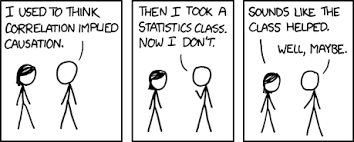
\includegraphics[width=0.75\linewidth]{images/causationcartoon}

Welcome to your guide to learning linear regression in Stata and R. This website houses all the information you need learn the basics of coding linear regression in Stata and R. It will not contain all the information taught in class, but will allow you to bridge that knowledge into running linear regressions on your own.

\hypertarget{labs}{%
\section{Labs}\label{labs}}

This is a 10-week course with 9 labs. Each lab will focus on some topic related to coding linear regression. By the end of the course, you should be able to run a linear regression project from start to finish with reproducible code.\\
Each lab will contain links to download script files (in .do or .r format), overviews of key concepts, and application questions.

\hypertarget{lab-topics}{%
\subsection*{Lab Topics}\label{lab-topics}}
\addcontentsline{toc}{subsection}{Lab Topics}

\begin{itemize}
\tightlist
\item
  Lab 1: Data cleaning review \& code annotation
\item
  Lab 2: Running a basic linear regression\\
\item
  Lab 3: Testing the assumptions of linear regression\\
\item
  Lab 4: Transforming variables \& displaying results
\item
  Lab 5: Exporting tables \& reproducible code
\item
  Lab 6: Evaluating linearity
\item
  Lab 7: Review \& requested topics TBD
\item
  Lab 8: Robust standard errors \& multicolinearity
\item
  Lab 9: Comparing models \& running a project from start to finish
\end{itemize}

\hypertarget{finding-data}{%
\section{Finding Data}\label{finding-data}}

\hypertarget{render-book}{%
\section{Render book}\label{render-book}}

You can render the HTML version of this example book without changing anything:

\begin{enumerate}
\def\labelenumi{\arabic{enumi}.}
\item
  Find the \textbf{Build} pane in the RStudio IDE, and
\item
  Click on \textbf{Build Book}, then select your output format, or select ``All formats'' if you'd like to use multiple formats from the same book source files.
\end{enumerate}

Or build the book from the R console:\texttt{\{r,\ eval=FALSE\}\ bookdown::render\_book()}

To render this example to PDF as a \texttt{bookdown::pdf\_book}, you'll need to install XeLaTeX. You are recommended to install TinyTeX (which includes XeLaTeX): \url{https://yihui.org/tinytex/}.

\hypertarget{preview-book}{%
\section{Preview book}\label{preview-book}}

As you work, you may start a local server to live preview this HTML book. This preview will update as you edit the book when you save individual .Rmd files. You can start the server in a work session by using the RStudio add-in ``Preview book'', or from the R console:\texttt{\{r\ eval=FALSE\}\ bookdown::serve\_book()}

\hypertarget{lab-1-stata}{%
\chapter{Lab 1 (Stata)}\label{lab-1-stata}}

\hypertarget{lab-goals-instructions}{%
\section{Lab Goals \& Instructions}\label{lab-goals-instructions}}

\begin{itemize}
\tightlist
\item
  Review the basics of data cleaning\\
\item
  Learn the importance of annotating code
\item
  Start develop your own coding style
\end{itemize}

\textbf{Instructions}

\begin{enumerate}
\def\labelenumi{\arabic{enumi}.}
\tightlist
\item
  Download the data file (\texttt{SOC401\_W21\_Billionaires.dta}) and .do script (\texttt{401-1-Lab1.do}) from the links below.
\item
  Create a file structure following \protect\hyperlink{file}{the instructions in 2.3 below}
\item
  Work through the .do script, executing each line of code. This page contains the same material, with more explanation about the functions used.
\item
  Read through the Importance of \protect\hyperlink{clean}{Annotation and Clean Code}, and complete the short activity at the bottom of the page. Email the .do script file to me by class on Monday.
\end{enumerate}

\textbf{Jump Links to Commands in this Lab:}\\
\protect\hyperlink{cd}{cd (set working directory)}\\
\protect\hyperlink{use}{use (load stata files)}\\
\protect\hyperlink{use}{import delimited (load .csv)}\\
\protect\hyperlink{describe}{describe}\\
\protect\hyperlink{mdesc}{mdesc for missing data}\\
\protect\hyperlink{summarize}{summarize}\\
\protect\hyperlink{tabulate}{tabulate}\\
\protect\hyperlink{generate}{generate}
\protect\hyperlink{recode}{recode}\\
\protect\hyperlink{replace}{replace}\\
\protect\hyperlink{histogram2}{histogram}\\
\protect\hyperlink{boxplot2}{graph box (box plot)}\\
\protect\hyperlink{barplot2}{graph bar (bar plot)}\\
\protect\hyperlink{keep}{keep}\\
\protect\hyperlink{drop}{drop}\\
\protect\hyperlink{saving}{save}\\
\protect\hyperlink{saving}{export delimited}

\hypertarget{lab-files}{%
\section{Lab Files}\label{lab-files}}

\hypertarget{file}{%
\section{Create a File Structure}\label{file}}

Life can get messy and so can data analysis. Creating a file structure is the equivalent of keeping a clean work space. You may not mind a messy desk, but a messy file structure will be a nightmare for your collaborators and increase your risk of making mistakes in your analysis. With quantitative data analysis, file management is crucial. I am going to suggest a file structure that you follow in this class. It will ensure that the relative pathways I include in lab script files will run.

For your first task, create the following file structure for this class.

\begin{enumerate}
\def\labelenumi{\arabic{enumi}.}
\tightlist
\item
  Decide where on your computer you'd like to store class files. Create a new folder in that spot titled anything you like. Example: 401\_Linear\_Regression. DO NOT include spaces in your folder title.
\item
  Create the following sub-folders in your main folder:
\end{enumerate}

\begin{itemize}
\tightlist
\item
  data\_raw
\item
  data\_work
\item
  scripts
\item
  figs\_output
\end{itemize}

\begin{enumerate}
\def\labelenumi{\arabic{enumi}.}
\setcounter{enumi}{2}
\tightlist
\item
  Move \texttt{SOC401\_W21\_Billionaires.dta} to your \texttt{data\_raw} folder.
\item
  Move \texttt{401-1-Lab1.do} to your \texttt{scripts} folder.
\end{enumerate}

When you begin labs, you should move all raw data files and script files to the appropriate locations.

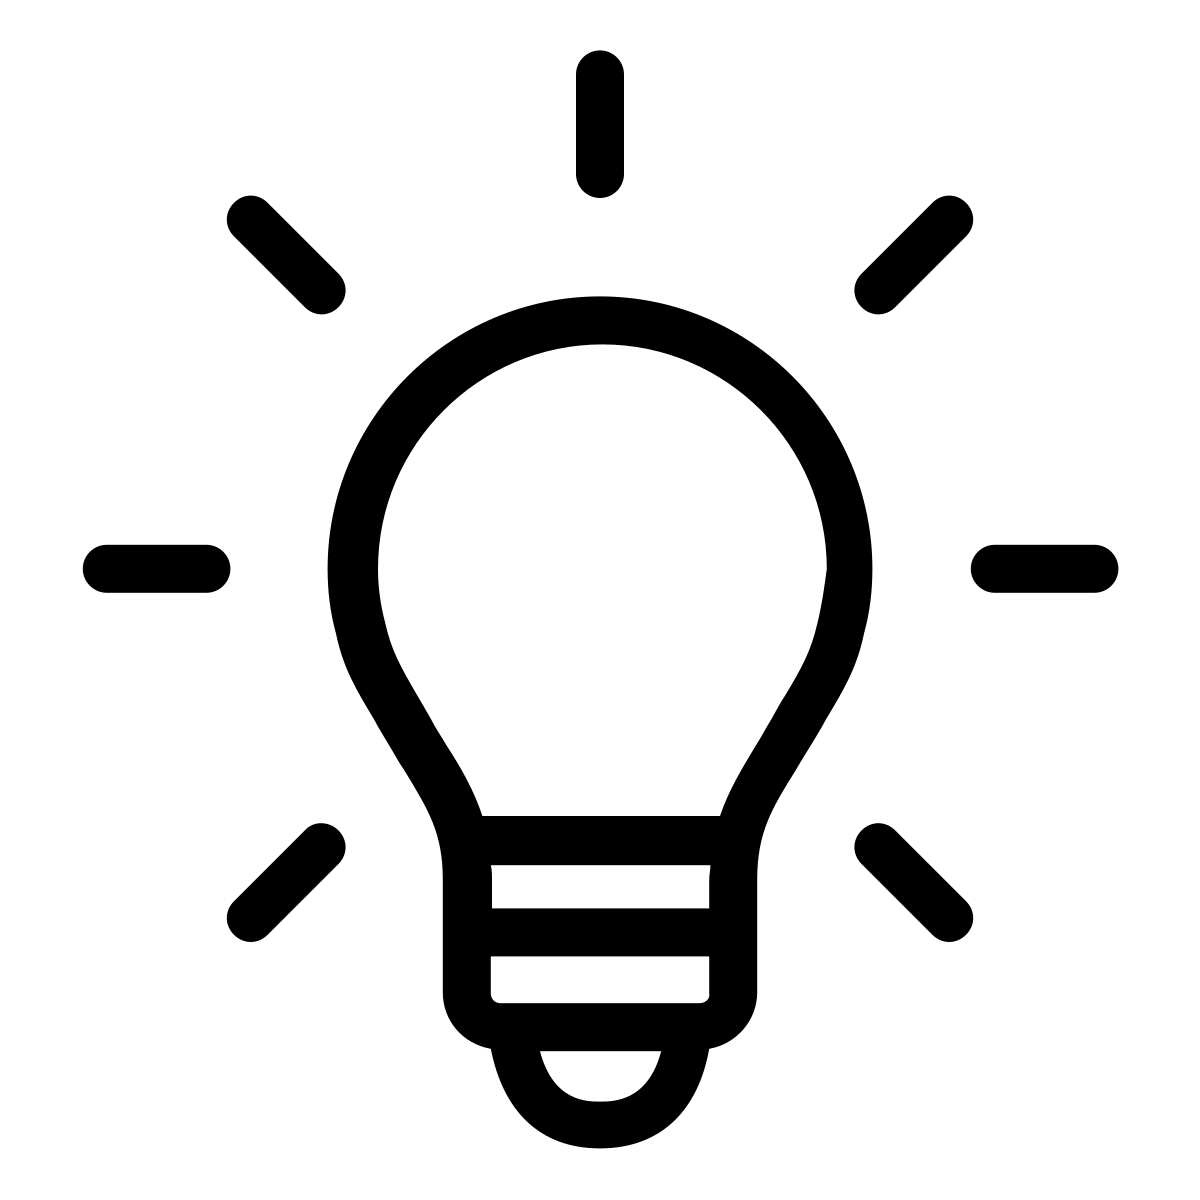
\includegraphics[width=0.36458in,height=\textheight]{images/bulb.png} Data Tip

\begin{quote}
Why do I need two separate folders for data?\\
You should aways store your original, raw data files in a place where they are in no danger of being saved over, altered, or lost. One great way of protecting your original data files is to create two folders for data: one folder for your raw files and one folder where you can saved cleaned datasets and subsets.
\end{quote}

\hypertarget{data-cleaning}{%
\section{Data Cleaning}\label{data-cleaning}}

95 percent of the work of quantitative research is getting your data in shape to run your model. This tutorial assumes that you opened Stata and run a few commands before. If you are have not used Stata before, here are some resources to help you get started coding in R.

\begin{itemize}
\tightlist
\item
  \href{https://www.princeton.edu/~otorres/StataTutorial.pdf}{Stata Tutorial from Princeton}: A great overview of Stata basics\\
\item
  \href{https://lo.unisa.edu.au/mod/book/view.php?id=641259}{Stata Tutorial from University of South Australia}
\item
  \href{https://www.stata.com/links/resources-for-learning-stata/cheat-sheets/StataCheatsheet_processing_June_2016_TE-REV.pdf}{Stata Commands Cheat Sheet}
\end{itemize}

Northwestern's Research Computing Services \href{https://www.it.northwestern.edu/research/training.html}{offers great trainings in a variety of software languages}. They do not have regular trainings in Stata, but you can set up individual meetings to help work through problems in your code. Check them out and get on their email list.

\hypertarget{cd}{%
\subsection*{Set up the environment}\label{cd}}
\addcontentsline{toc}{subsection}{Set up the environment}

\textbf{Working Directory}\\
Before you get to work cleaning your data, you need to let the software know where to grab and save your files. This saves you from having to type in a long file path anytime you want to do something. You must begin any Stata .do file by setting your working directory. Your working directory is the folder on your computer where you want to store all your data and script files. Below you will see the path to my working directory. You should replace the filepath with the one you want to use.

\begin{Shaded}
\begin{Highlighting}[]
\NormalTok{cd }\StringTok{"/Users/srwerth/Documents/Work\_Research/Regression\_Labs"}
\end{Highlighting}
\end{Shaded}

\textbf{Do File Set-up}\\
Now that you've set your working directory, you can tell Stata to go grab your data and load it into your working environment.
There are a couple lines of code you want to put at the beginning of your .do file to keep your code running smoothly.

\begin{itemize}
\tightlist
\item
  \texttt{clear\ all}: Clears the stata environment before you run your code.
\item
  \texttt{capture\ log\ close}: If there's a previous log set up, this code closes it.
\item
  \texttt{log\ using\ Lab1.scl,\ replace}: This creates a new log file, which is a file that tracks all the code you run in the session. This is important for reviewing your analysis after the fact. Rename the file whatever you like for each lab.
\item
  \texttt{version\ 17}: This command Stata what version of the software you wrote this .do file in, in case you are running
  it in a different version later. Sometimes commands can change between versions. This prevents any inconsistencies between versions from causing errors.
\end{itemize}

\begin{Shaded}
\begin{Highlighting}[]
\KeywordTok{clear} \OtherTok{all} 
\KeywordTok{capture} \FunctionTok{log} \KeywordTok{close}
\FunctionTok{log} \KeywordTok{using}\NormalTok{ Lab1.smcl, }\KeywordTok{replace}
\KeywordTok{version}\NormalTok{ 17}
\end{Highlighting}
\end{Shaded}

\hypertarget{use}{%
\subsection{Load your data}\label{use}}

Now you are ready to load your data. Loading data that is in Stata's data formats is easy. An Stata data file ends in .dta. Note how I get to use a relative path, just telling Stata to look in the \texttt{data\_raw} folder, and then the dataset name.

\begin{Shaded}
\begin{Highlighting}[]
\KeywordTok{use} \StringTok{"data\_raw/SOC401\_W21\_Billionaires.dta"}
\end{Highlighting}
\end{Shaded}

You can also load data in other formats. A CSV file is one of the most common data formats.

\begin{Shaded}
\begin{Highlighting}[]
\NormalTok{import delimited }\StringTok{"data\_raw/SOC401\_W21\_Billionaires.csv"}
\end{Highlighting}
\end{Shaded}

Check out this tutorial on how to load excel data:
\url{https://www.stata.com/manuals/dimportexcel.pdf}

\hypertarget{exploring-your-data}{%
\subsection*{Exploring your data}\label{exploring-your-data}}
\addcontentsline{toc}{subsection}{Exploring your data}

When you begin any new project, it is important to understand the condition of your variables. Here are a few important functions you need to begin that process.

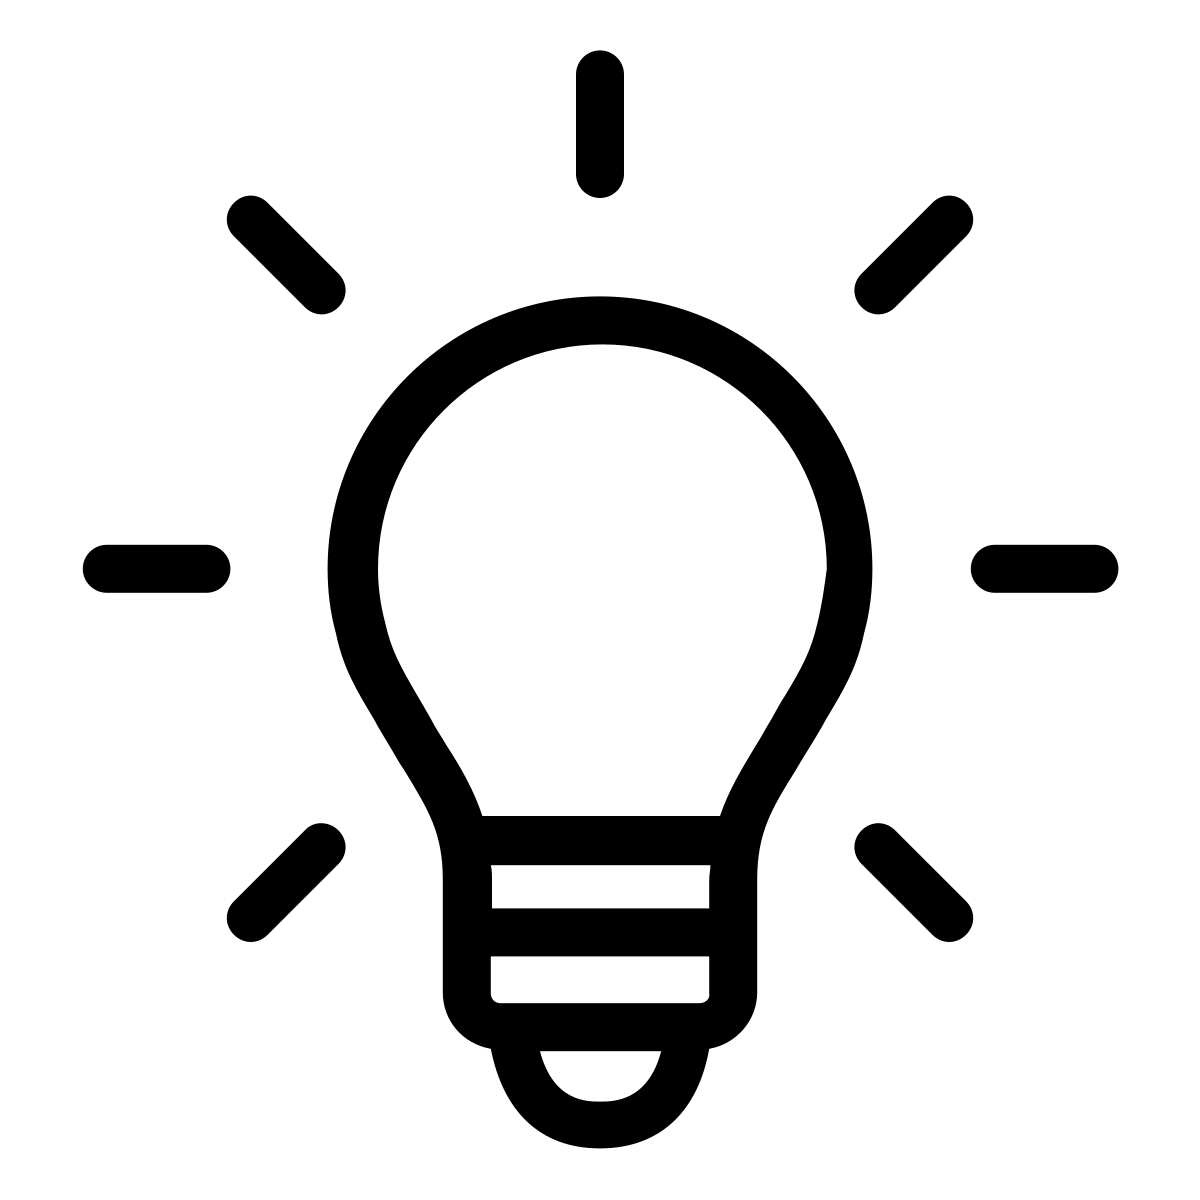
\includegraphics[width=0.36458in,height=\textheight]{images/bulb.png} Data Tip

\begin{quote}
Remember if this script or any other uses a command that you are not familiar with, you can search for the function online or type `help' and then the name of the function you want to look up in the command line. For example, `help describe' will pull up the documentation for that command.
\end{quote}

\hypertarget{describe}{%
\subsubsection*{Let's start by taking a global look at your dataset.}\label{describe}}
\addcontentsline{toc}{subsubsection}{Let's start by taking a global look at your dataset.}

The \texttt{describe} function provides an overview of your dataset. The output includes the number of observations, variables, and a description of each variable in the dataset. The description includes the format and any labels already attached to each variable.

\begin{Shaded}
\begin{Highlighting}[]
\KeywordTok{describe}
\end{Highlighting}
\end{Shaded}

\begin{verbatim}
Contains data from data_raw/SOC401_W21_Billionaires.dta
 Observations:         2,614                  
    Variables:            21                  9 Jan 2021 15:56
----------------------------------------------------------------------------------
Variable      Storage   Display    Value
    name         type    format    label      Variable label
----------------------------------------------------------------------------------
name            str45   %45s                  
rank            int     %8.0g                 
year            int     %8.0g                 
companyfounded  int     %8.0g                 company.founded
companyname     str59   %59s                  company.name
demographicsage byte    %8.0g                 demographics.age
locationgdp     double  %10.0g                location.gdp
wealthworthin~s float   %9.0g                 wealth.worth in billions
wealthhowfrom~g str4    %9s                   wealth.how.from emerging
wealthhowwasf~r str4    %9s                   wealth.how.was founder
wealthhowwasp~l str4    %9s                   wealth.how.was political
wealthhowinhe~2 long    %24.0g     wealthhowinherited2
                                              wealth.how.inherited
wealthhowcate~2 long    %18.0g     wealthhowcategory2
                                              wealth.how.category
wealthtype2     long    %24.0g     wealthtype2
                                              wealth.type
wealthhowindu~2 long    %31.0g     wealthhowindustry2
                                              wealth.how.industry
locationregion2 long    %24.0g     locationregion2
                                              location.region
locationcount~2 long    %8.0g      locationcountrycode2
                                              location.country code
locationcitiz~2 long    %20.0g     locationcitizenship2
                                              location.citizenship
demographicsg~2 long    %14.0g     demographicsgender2
                                              demographics.gender
companysector2  long    %52.0g     companysector2
                                              company.sector
companyrelati~2 long    %46.0g     companyrelationship2
                                              company.relationship
----------------------------------------------------------------------------------
Sorted by: 
\end{verbatim}

You can also look at a specific variable you want to learn more about

\begin{Shaded}
\begin{Highlighting}[]
\KeywordTok{describe}\NormalTok{ demographicsgender2}
\end{Highlighting}
\end{Shaded}

\begin{verbatim}
Variable      Storage   Display    Value
    name         type    format    label      Variable label
----------------------------------------------------------------------------------
demographicsg~2 long    %14.0g     demographicsgender2
                                              demographics.gender
\end{verbatim}

If you want to look at your data set in a spreadsheet-type format you can look at the Data Editor in browse mode. You can open the Data Editor by clicking on the icon below on the top bar. Make sure you click on the icon with the magnifying glass (browse mode), not the pencil (edit mode). You do not want to accidentally edit your data.


\includegraphics[width=4.16667in,height=\textheight]{images/data_editor.png}

\hypertarget{mdesc}{%
\subsubsection*{Look at missing observations in your dataset}\label{mdesc}}
\addcontentsline{toc}{subsubsection}{Look at missing observations in your dataset}

To look at missing values for each variable in your data set we need to download a new function into Stata. The \texttt{mdesc} function makes looking at missing values easy. To install a Stata program you can run \texttt{search\ mdesc} in the command line and click the link in the program information to install the program ()

\begin{Shaded}
\begin{Highlighting}[]
\KeywordTok{ssc}\NormalTok{ install mdesc}
\end{Highlighting}
\end{Shaded}

Now you are ready to look at the missing values in your dataset

\begin{Shaded}
\begin{Highlighting}[]
\NormalTok{mdesc}
\end{Highlighting}
\end{Shaded}

\begin{verbatim}
    Variable    |     Missing          Total     Percent Missing
----------------+-----------------------------------------------
           name |           0          2,614           0.00
           rank |           0          2,614           0.00
           year |           0          2,614           0.00
   companyfou~d |           0          2,614           0.00
    companyname |          38          2,614           1.45
   demographi~e |           0          2,614           0.00
    locationgdp |           0          2,614           0.00
   wealthwort~s |           0          2,614           0.00
   wealthhowf~g |           0          2,614           0.00
   wealthhoww~r |           0          2,614           0.00
   wealthhoww~l |           0          2,614           0.00
   wealthhow~d2 |           0          2,614           0.00
   wealthhowc~2 |           1          2,614           0.04
    wealthtype2 |          22          2,614           0.84
   wealthh~try2 |           1          2,614           0.04
   locationre~2 |           0          2,614           0.00
   locationco~2 |           0          2,614           0.00
   locationci~2 |           0          2,614           0.00
   demographi~2 |          34          2,614           1.30
   companysec~2 |          23          2,614           0.88
   companyrel~2 |          46          2,614           1.76
----------------+-----------------------------------------------
\end{verbatim}

Or you can look at missing values for a specific variable

\begin{Shaded}
\begin{Highlighting}[]
\NormalTok{mdesc companyname}
\end{Highlighting}
\end{Shaded}

\begin{verbatim}
    Variable    |     Missing          Total     Percent Missing
----------------+-----------------------------------------------
    companyname |          38          2,614           1.45
----------------+-----------------------------------------------
\end{verbatim}

\hypertarget{summarize}{%
\subsubsection*{\texorpdfstring{Descriptive statistics for continous variables using \texttt{summarize}}{Descriptive statistics for continous variables using summarize}}\label{summarize}}
\addcontentsline{toc}{subsubsection}{Descriptive statistics for continous variables using \texttt{summarize}}

You can generate simple descriptive statistics (mean, standard deviation, range, etc.) with the \texttt{summarize} command. Looking at descriptive statistics is not only helpful to get a sense of your data, they can also be helpful checks as you work on cleaning a dataset.

\begin{Shaded}
\begin{Highlighting}[]
\KeywordTok{summarize}\NormalTok{ demographicsage}
\end{Highlighting}
\end{Shaded}

\begin{verbatim}
    Variable |        Obs        Mean    Std. dev.       Min        Max
-------------+---------------------------------------------------------
demographi~e |      2,614    53.34124    25.33332        -42         98
\end{verbatim}

If you add \texttt{,\ detail} to the command youcan see additional descriptive statistics,
including skew, variance and quartiles.

\begin{Shaded}
\begin{Highlighting}[]
\KeywordTok{summarize}\NormalTok{ demographicsage, }\KeywordTok{detail}
\end{Highlighting}
\end{Shaded}

\begin{verbatim}
                      demographics.age
-------------------------------------------------------------
      Percentiles      Smallest
 1%            0            -42
 5%            0             -7
10%            0              0       Obs               2,614
25%           47              0       Sum of wgt.       2,614

50%           59                      Mean           53.34124
                        Largest       Std. dev.      25.33332
75%           70             95
90%           79             96       Variance       641.7771
95%           84             96       Skewness      -1.104472
99%           90             98       Kurtosis       3.330685
\end{verbatim}

\hypertarget{tabulate}{%
\subsubsection*{\texorpdfstring{Frequency tables for categorical variables using \texttt{tabulate}}{Frequency tables for categorical variables using tabulate}}\label{tabulate}}
\addcontentsline{toc}{subsubsection}{Frequency tables for categorical variables using \texttt{tabulate}}

Tabulate produces a frequency table showing how many observations there are for each value.

\begin{Shaded}
\begin{Highlighting}[]
\KeywordTok{tabulate}\NormalTok{ demographicsgender2}
\end{Highlighting}
\end{Shaded}

\begin{verbatim}
demographics.g |
         ender |      Freq.     Percent        Cum.
---------------+-----------------------------------
        female |        249        9.65        9.65
          male |      2,328       90.23       99.88
married couple |          3        0.12      100.00
---------------+-----------------------------------
         Total |      2,580      100.00
\end{verbatim}

If you add \texttt{,\ nolabel} it shows you the values without their label. This is how the values appear in the actual data, which is important to know when you have to recode your data. With this example, you can see that female is coded as 1, male is coded as 2, and married couple is coded as 3.

\begin{Shaded}
\begin{Highlighting}[]
\KeywordTok{tabulate}\NormalTok{ demographicsgender2, }\KeywordTok{nolabel}
\end{Highlighting}
\end{Shaded}

\begin{verbatim}
demographic |
   s.gender |      Freq.     Percent        Cum.
------------+-----------------------------------
          1 |        249        9.65        9.65
          2 |      2,328       90.23       99.88
          3 |          3        0.12      100.00
------------+-----------------------------------
      Total |      2,580      100.00
\end{verbatim}

If you add \texttt{,\ missing} it will add a row to the table showing the number of missing values for that variable.

\begin{Shaded}
\begin{Highlighting}[]
\KeywordTok{tabulate}\NormalTok{ demographicsgender2, }\FunctionTok{missing}
\end{Highlighting}
\end{Shaded}

\begin{verbatim}
demographics.g |
         ender |      Freq.     Percent        Cum.
---------------+-----------------------------------
        female |        249        9.53        9.53
          male |      2,328       89.06       98.58
married couple |          3        0.11       98.70
             . |         34        1.30      100.00
---------------+-----------------------------------
         Total |      2,614      100.00
\end{verbatim}

\textbf{Note:} you can also shorten \texttt{tabulate} to \texttt{tab} and the function will run the same.

\hypertarget{cleaning-variables}{%
\subsection*{Cleaning variables}\label{cleaning-variables}}
\addcontentsline{toc}{subsection}{Cleaning variables}

In the previous section, we learn the code to check the state of a variable when we first open the dataset. Most of the time, you're likely to find that the variable isn't ideal to work with. It is important to use this commands to make a variable ready for your use.

Let's take a closer look at the variable for gender again:

\begin{Shaded}
\begin{Highlighting}[]
\KeywordTok{tabulate}\NormalTok{ demographicsgender2}
\end{Highlighting}
\end{Shaded}

\begin{verbatim}
demographics.g |
         ender |      Freq.     Percent        Cum.
---------------+-----------------------------------
        female |        249        9.65        9.65
          male |      2,328       90.23       99.88
married couple |          3        0.12      100.00
---------------+-----------------------------------
         Total |      2,580      100.00
\end{verbatim}

I notice a few things you will want to change about that variable:

\begin{enumerate}
\def\labelenumi{\alph{enumi})}
\tightlist
\item
  The variable name is tedious to type
\item
  We want this to be a dummy variable where 1 is female and 0 is not female (in this binary, male).
\item
  We have three married couples in our data set coded as 3
\end{enumerate}

Let's create a new variable with a better name and recode it how you'd like it.

\hypertarget{generate}{%
\subsubsection*{\texorpdfstring{\texttt{generate} to create new variables}{generate to create new variables}}\label{generate}}
\addcontentsline{toc}{subsubsection}{\texttt{generate} to create new variables}

If you want to label the 3 married couples as 0, aka not female, take the following steps. First let's generate a new variable \texttt{female} with the same values as \texttt{demographicsgender2}. We'll also go ahead and label that variable ``Female''.

\begin{Shaded}
\begin{Highlighting}[]
\KeywordTok{gen}\NormalTok{ female = demographicsgender2}
\KeywordTok{label} \KeywordTok{variable}\NormalTok{ female }\StringTok{"Female (recoded)"}
\end{Highlighting}
\end{Shaded}

The command is \texttt{label\ variable}, the variable you are labeling is \texttt{female}, and the label is ``Female''.

\hypertarget{recode}{%
\subsubsection*{\texorpdfstring{\texttt{recode} to transform the values of a variable}{recode to transform the values of a variable}}\label{recode}}
\addcontentsline{toc}{subsubsection}{\texttt{recode} to transform the values of a variable}

Now let's take our new variable and recode the values so that 0 means ``Not Female'' and 1 means ``Female''. In this example, we're taking all the married couples and labeling them as 0. In this code you are telling Stata to recode the variable \texttt{female} so that a 3 becomes a 0, a 2 becomes a 0 and a 1 stays a 1.

\begin{Shaded}
\begin{Highlighting}[]
\KeywordTok{recode}\NormalTok{ female (3 = 0) (2 = 0) (1 = 1) }
\end{Highlighting}
\end{Shaded}

You should also at this point apply a label to these new values, so your tables and graphs will be easier to read. This is a two step process. First you create an object that stores the labels you want to apply to each value. \texttt{label\ define} is the command and \texttt{gender} is the name of the object you are creating.

\begin{Shaded}
\begin{Highlighting}[]
\KeywordTok{label} \KeywordTok{define}\NormalTok{ gender 0 }\StringTok{"Not Female"}\NormalTok{ 1 }\StringTok{"Female"}
\end{Highlighting}
\end{Shaded}

Second, you apply that label object to the variable. \texttt{label\ values} is the command, \texttt{female} is the name of the variable you want to label, and \texttt{gender} is the label object you want to apply to it.

\begin{Shaded}
\begin{Highlighting}[]
\KeywordTok{label} \KeywordTok{values}\NormalTok{ female gender}
\end{Highlighting}
\end{Shaded}

Let's run a crosstab table to make sure that everything came out right. Looks like everything landed where it is supposed to.

\begin{Shaded}
\begin{Highlighting}[]
\KeywordTok{tab}\NormalTok{ female demographicsgender2}
\end{Highlighting}
\end{Shaded}

\begin{verbatim}
    Female |       demographics.gender
 (recoded) |    female       male  married c |     Total
-----------+---------------------------------+----------
Not Female |         0      2,328          3 |     2,331 
    Female |       249          0          0 |       249 
-----------+---------------------------------+----------
     Total |       249      2,328          3 |     2,580 
\end{verbatim}

\hypertarget{replace}{%
\subsubsection*{\texorpdfstring{\texttt{replace} to transform the values of a variable}{replace to transform the values of a variable}}\label{replace}}
\addcontentsline{toc}{subsubsection}{\texttt{replace} to transform the values of a variable}

There's another way to recode variables. Both options work just as well, so it is truly your preference which one you want to use. We'll practice using the replace command by recoding our gender variable a different way. Let's make a new variable so 0 only refers to ``Male'' and 1 only refers to ``Female''. You will recode the married couples to missing.

First, you will generate a new variable, \texttt{female2}. In this instance we set all the values of the new variable to missing. We'll also label it.

\begin{Shaded}
\begin{Highlighting}[]
\KeywordTok{gen}\NormalTok{ female2 = . }
\KeywordTok{label} \KeywordTok{variable}\NormalTok{ female2 }\StringTok{"Female (Male/Female)"}
\end{Highlighting}
\end{Shaded}

Now let's recode our values using the replace command. This command replaces the values of your variable, based on the values of another variable. Here you are telling Stata to replace the value of \texttt{female2} if \texttt{demographicsgender2} is equal to 2. On the second line you make the value of \texttt{female2} 1 if \texttt{demographicsgender} is equal to 1.

\begin{Shaded}
\begin{Highlighting}[]
\KeywordTok{replace}\NormalTok{ female2 = 0 }\KeywordTok{if}\NormalTok{ demographicsgender2 == 2 }
\KeywordTok{replace}\NormalTok{ female2 = 1 }\KeywordTok{if}\NormalTok{ demographicsgender2 == 1}
\end{Highlighting}
\end{Shaded}

Let's label it as well

\begin{Shaded}
\begin{Highlighting}[]
\KeywordTok{label} \KeywordTok{define}\NormalTok{ gender2 0 }\StringTok{"Male"}\NormalTok{ 1 }\StringTok{"Female"}
\KeywordTok{label} \KeywordTok{values}\NormalTok{ female2 gender2}
\end{Highlighting}
\end{Shaded}

Because you set all the values to missing and do not recode the 3 values to anything, they will remain missing. Let's double check with our crosstab using \texttt{tabulate}. We'll add \texttt{,\ missing} to see if the 3 values were recoded correctly (and everything looks good).

\begin{Shaded}
\begin{Highlighting}[]
\KeywordTok{tab}\NormalTok{ female2 demographicsgender2, }\FunctionTok{missing}
\end{Highlighting}
\end{Shaded}

\begin{verbatim}
    Female |
(Male/Fema |             demographics.gender
       le) |    female       male  married c          . |     Total
-----------+--------------------------------------------+----------
      Male |         0      2,328          0          0 |     2,328 
    Female |       249          0          0          0 |       249 
         . |         0          0          3         34 |        37 
-----------+--------------------------------------------+----------
     Total |       249      2,328          3         34 |     2,614 
\end{verbatim}

\textbf{Note}: In Stata when you are creating something new, as with the generate, you use a single equals sign. Your new variable \texttt{female} \emph{should equal} what follows. When you're writing a test statement referring to something that already exists, you use double equals sign (\texttt{==}), as we do in the second part of the replace command. .

Now let's try another example, looking at the variable for age:

\begin{Shaded}
\begin{Highlighting}[]
\KeywordTok{tab}\NormalTok{ demographicsage, }\FunctionTok{missing}
\end{Highlighting}
\end{Shaded}

\begin{verbatim}
demographic |
      s.age |      Freq.     Percent        Cum.
------------+-----------------------------------
        -42 |          1        0.04        0.04
         -7 |          1        0.04        0.08
          0 |        383       14.65       14.73
         12 |          1        0.04       14.77
         21 |          1        0.04       14.80
         24 |          2        0.08       14.88
         28 |          2        0.08       14.96
         29 |          4        0.15       15.11
         30 |          4        0.15       15.26
         31 |          5        0.19       15.46
         32 |          4        0.15       15.61
         33 |          8        0.31       15.91
         34 |          6        0.23       16.14
         35 |          8        0.31       16.45
         36 |          7        0.27       16.72
         37 |          8        0.31       17.02
         38 |          7        0.27       17.29
         39 |         10        0.38       17.67
         40 |         13        0.50       18.17
         41 |         15        0.57       18.75
         42 |         18        0.69       19.43
         43 |         19        0.73       20.16
         44 |         25        0.96       21.12
         45 |         29        1.11       22.23
         46 |         42        1.61       23.83
         47 |         35        1.34       25.17
         48 |         46        1.76       26.93
         49 |         57        2.18       29.11
         50 |         65        2.49       31.60
         51 |         42        1.61       33.21
         52 |         54        2.07       35.27
         53 |         44        1.68       36.95
         54 |         47        1.80       38.75
         55 |         63        2.41       41.16
         56 |         55        2.10       43.27
         57 |         60        2.30       45.56
         58 |         63        2.41       47.97
         59 |         61        2.33       50.31
         60 |         76        2.91       53.21
         61 |         54        2.07       55.28
         62 |         64        2.45       57.73
         63 |         61        2.33       60.06
         64 |         65        2.49       62.55
         65 |         52        1.99       64.54
         66 |         56        2.14       66.68
         67 |         50        1.91       68.59
         68 |         64        2.45       71.04
         69 |         65        2.49       73.53
         70 |         59        2.26       75.78
         71 |         55        2.10       77.89
         72 |         59        2.26       80.15
         73 |         52        1.99       82.13
         74 |         46        1.76       83.89
         75 |         36        1.38       85.27
         76 |         45        1.72       86.99
         77 |         43        1.64       88.64
         78 |         30        1.15       89.79
         79 |         26        0.99       90.78
         80 |         21        0.80       91.58
         81 |         28        1.07       92.65
         82 |         24        0.92       93.57
         83 |         26        0.99       94.57
         84 |         20        0.77       95.33
         85 |         25        0.96       96.29
         86 |         21        0.80       97.09
         87 |         18        0.69       97.78
         88 |         17        0.65       98.43
         89 |          7        0.27       98.70
         90 |         12        0.46       99.16
         91 |          4        0.15       99.31
         92 |          6        0.23       99.54
         93 |          4        0.15       99.69
         94 |          3        0.11       99.81
         95 |          2        0.08       99.89
         96 |          2        0.08       99.96
         98 |          1        0.04      100.00
------------+-----------------------------------
      Total |      2,614      100.00
\end{verbatim}

The major concern is that there are some numbers that seem unreasonable. Age is not negative, and 0 is an unlikely age for a person in a billionaire dataset. Let's recode those variables to missing (.) for now. First we generate a new variable named something simpler and easier to type and label it.

\begin{Shaded}
\begin{Highlighting}[]
\KeywordTok{generate}\NormalTok{ age = demographicsage}
\KeywordTok{label} \KeywordTok{variable}\NormalTok{ age }\StringTok{"Age (recoded)"}
\end{Highlighting}
\end{Shaded}

Now you'll use \texttt{recode} to set any values 0 or below to missing.

\begin{Shaded}
\begin{Highlighting}[]
\KeywordTok{replace}\NormalTok{ age = . }\KeywordTok{if}\NormalTok{ age \textless{}= 0}
\end{Highlighting}
\end{Shaded}

Use \texttt{summarize} to check the new range.

\begin{Shaded}
\begin{Highlighting}[]
\KeywordTok{summarize}\NormalTok{ age }
\end{Highlighting}
\end{Shaded}

\begin{verbatim}
    Variable |        Obs        Mean    Std. dev.       Min        Max
-------------+---------------------------------------------------------
         age |      2,229    62.57649    13.13472         12         98
\end{verbatim}

Use \texttt{mdesc} to check the new number of missing values. 385 is equal to all the previous 0, -7, and -42 values.

\begin{Shaded}
\begin{Highlighting}[]
\NormalTok{mdesc age}
\end{Highlighting}
\end{Shaded}

\begin{verbatim}
    Variable    |     Missing          Total     Percent Missing
----------------+-----------------------------------------------
            age |         385          2,614          14.73
----------------+-----------------------------------------------
\end{verbatim}

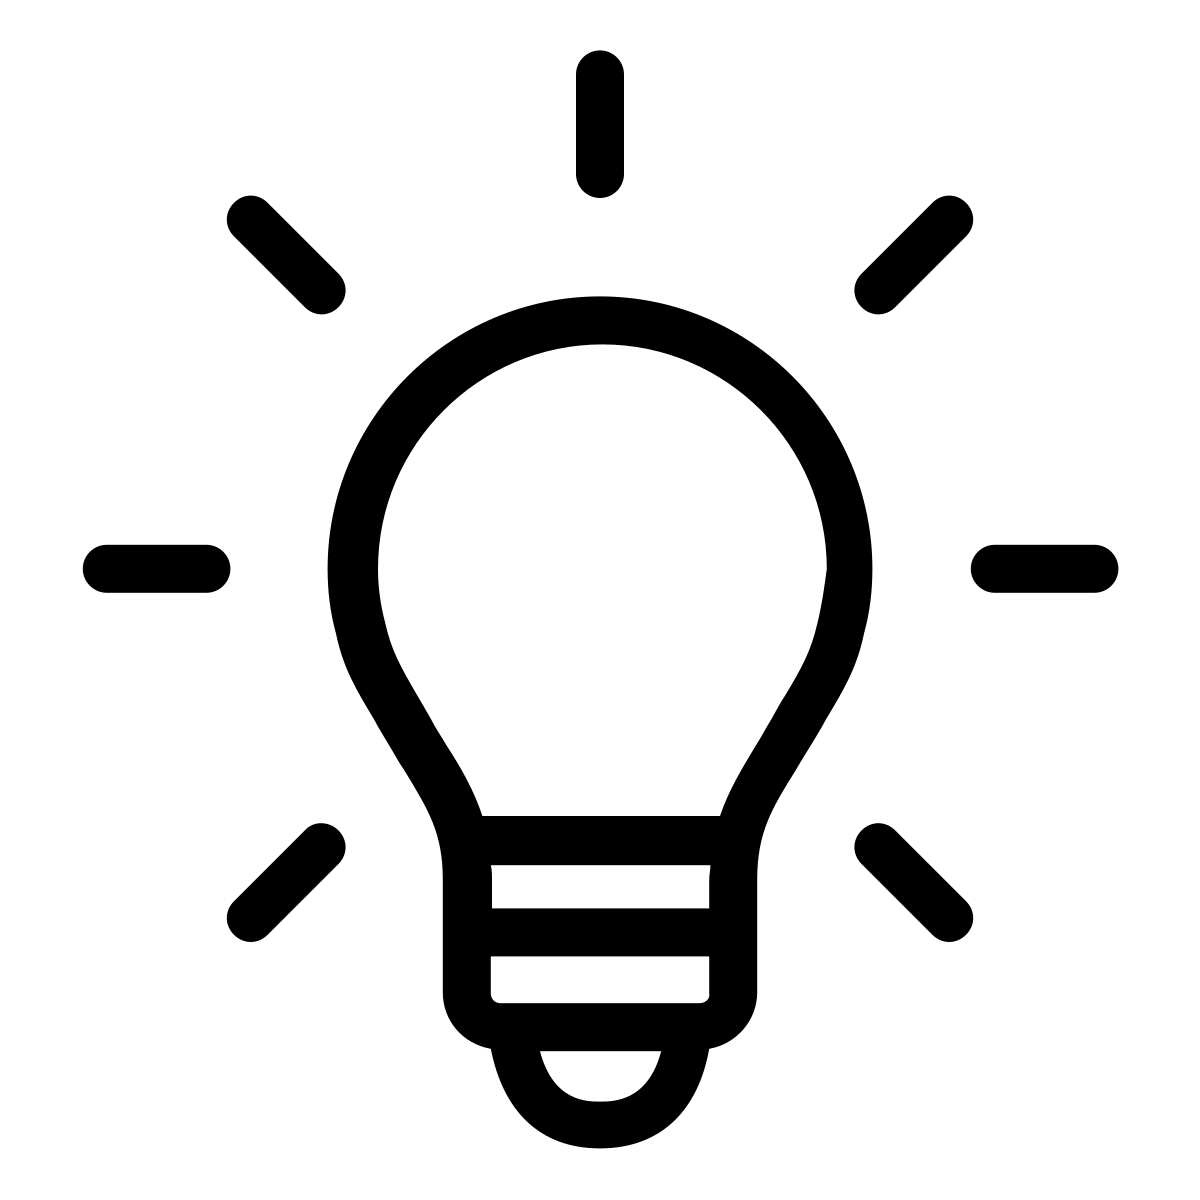
\includegraphics[width=0.36458in,height=\textheight]{images/bulb.png} Data Tip

\begin{quote}
\textbf{Why create a new variable when recoding?}\\
If you have a sharp eye, you'll notice that we created a new variable rather than changing the name of our original variable and recoding it. Data cleaning is an iterative process. You may make mistakes (you will probably make mistakes) or you may change your mind about how to recode a variable. In each case, having the original variable on hand is always helpful. To preserve your original variable, you create a new variable rather than writing over the old one.
\end{quote}

\hypertarget{vizualizing-variables}{%
\subsection*{Vizualizing variables}\label{vizualizing-variables}}
\addcontentsline{toc}{subsection}{Vizualizing variables}

\hypertarget{continuous-variables}{%
\subsubsection*{Continuous Variables}\label{continuous-variables}}
\addcontentsline{toc}{subsubsection}{Continuous Variables}

While frequency tables and descriptive statistics are helpful, visualizing continuous variables or discrete variables with a wide range of values can be helpful to get a look at the shape of our data. Histograms or box plots the go to.

\hypertarget{histogram2}{%
\paragraph*{Histograms}\label{histogram2}}
\addcontentsline{toc}{paragraph}{Histograms}

\begin{Shaded}
\begin{Highlighting}[]
\KeywordTok{histogram}\NormalTok{ age }
\end{Highlighting}
\end{Shaded}

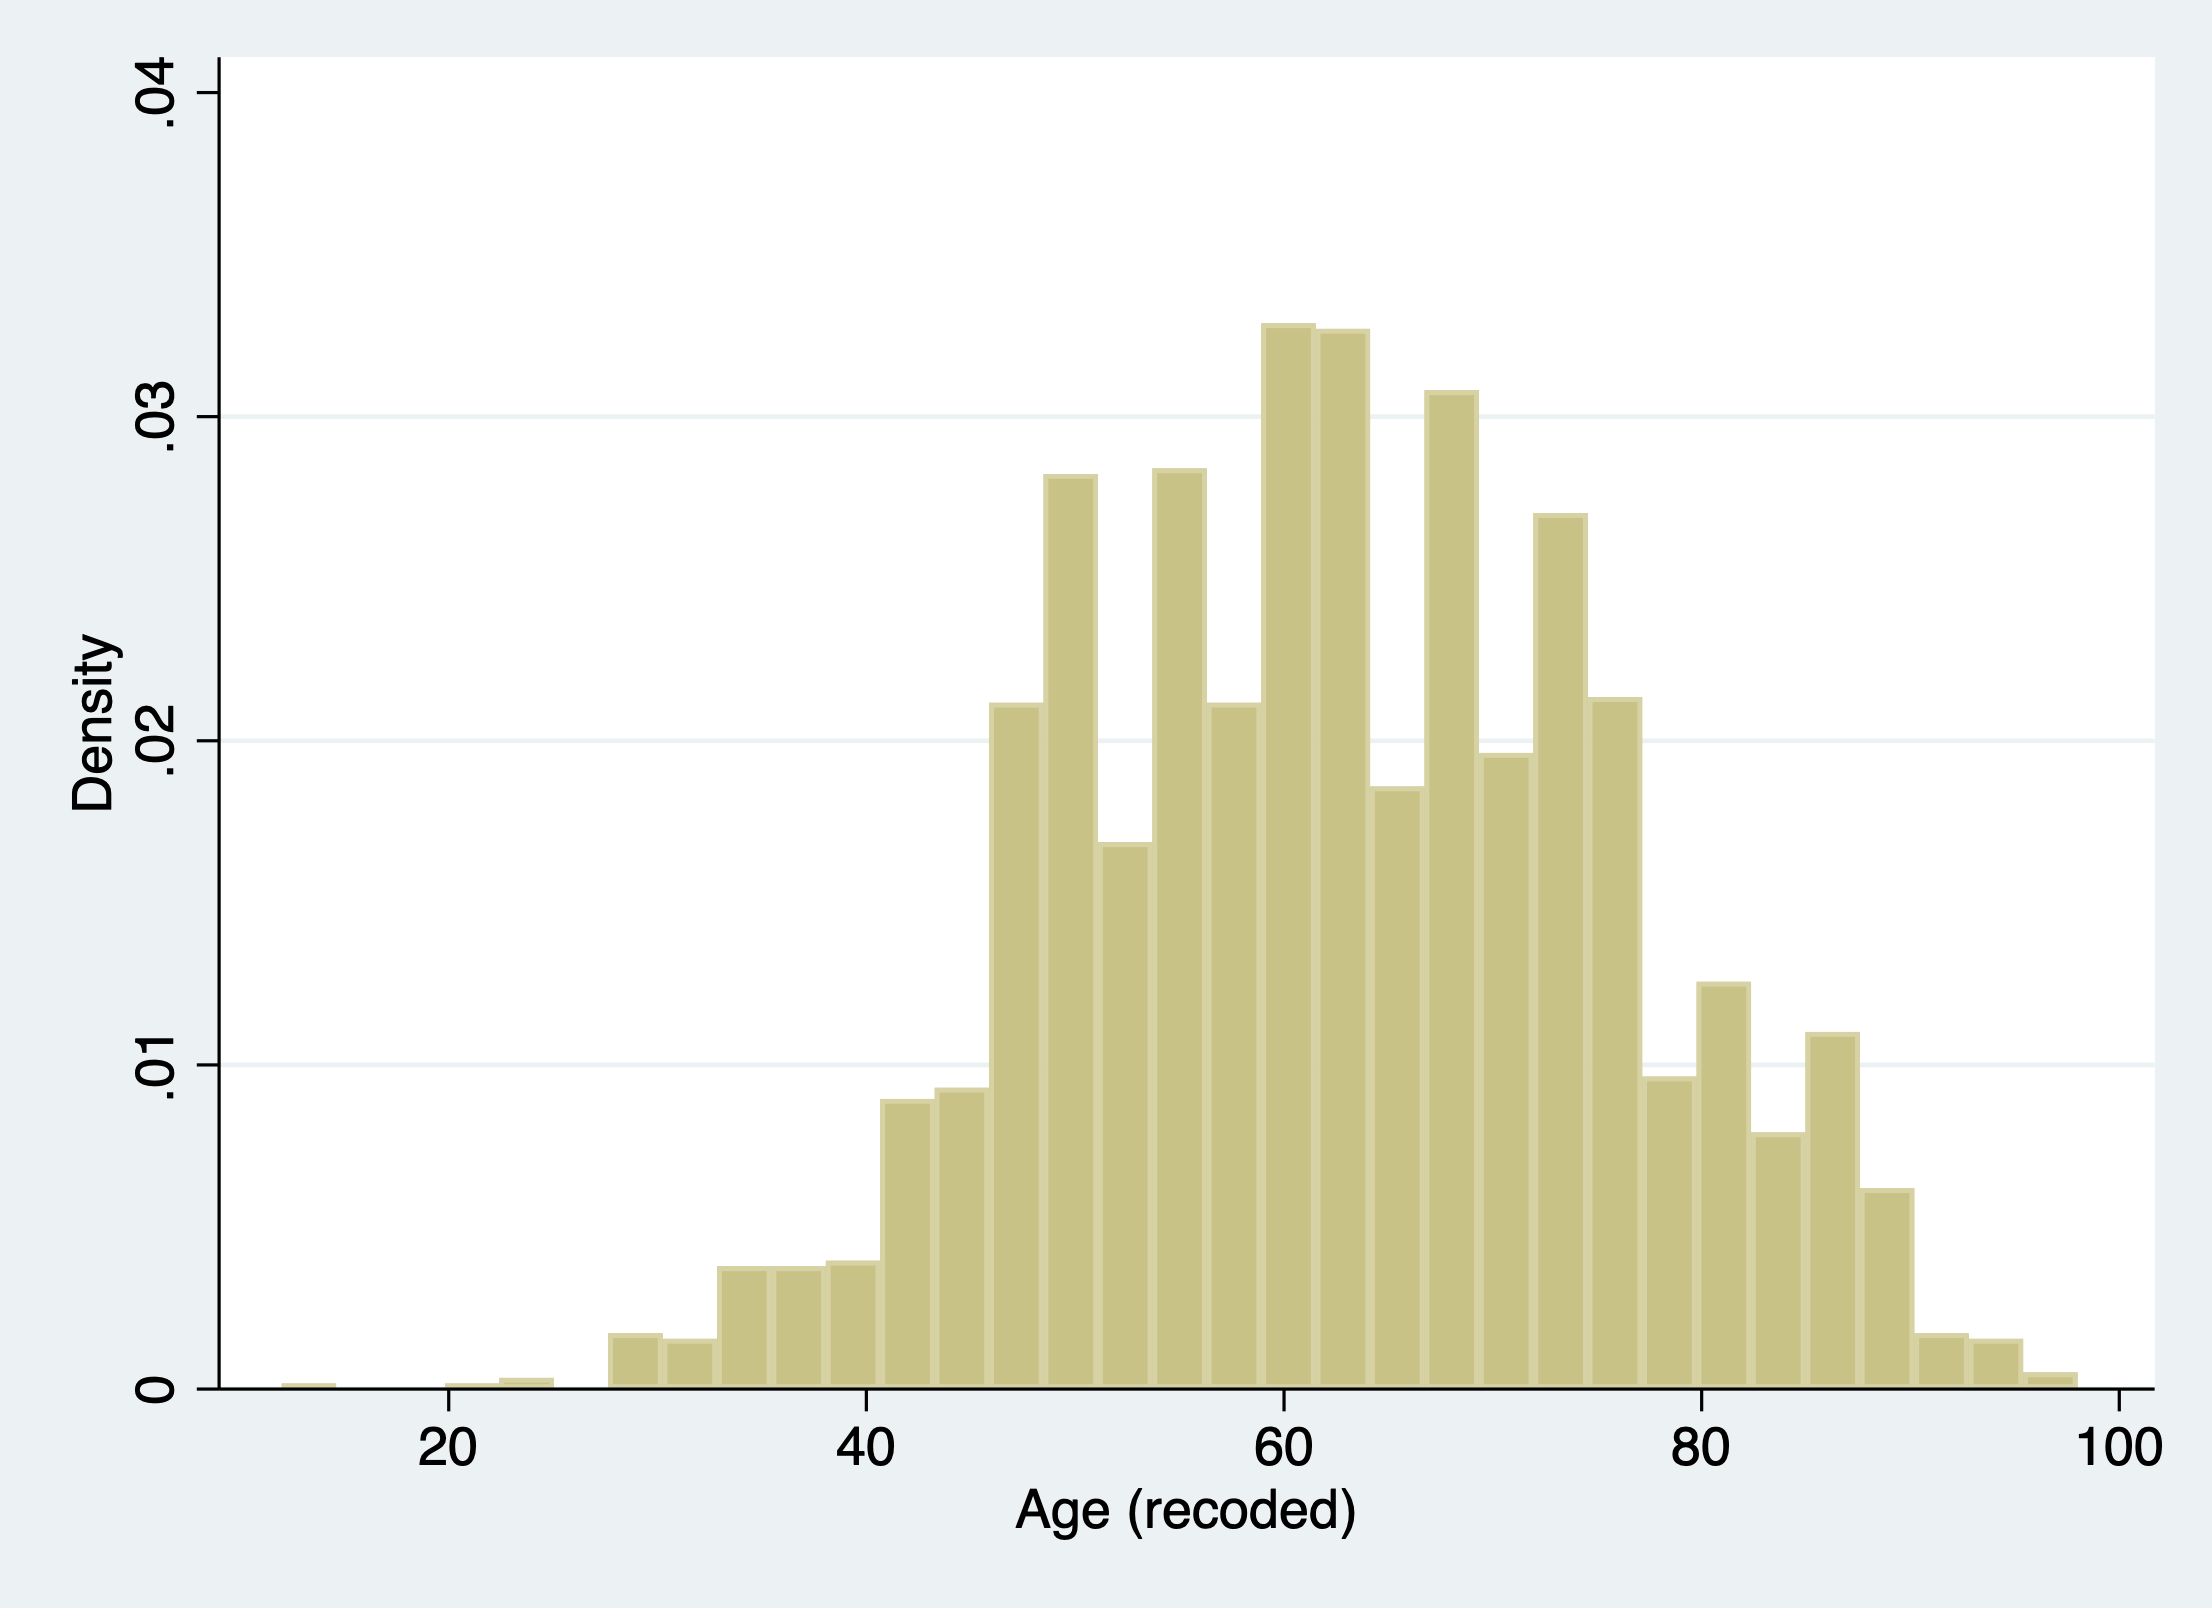
\includegraphics{images/histogram_stata.png}

If you want to change the number of bins (i.e.~bars),

\begin{Shaded}
\begin{Highlighting}[]
\KeywordTok{histogram}\NormalTok{ age, bins(10)}
\end{Highlighting}
\end{Shaded}

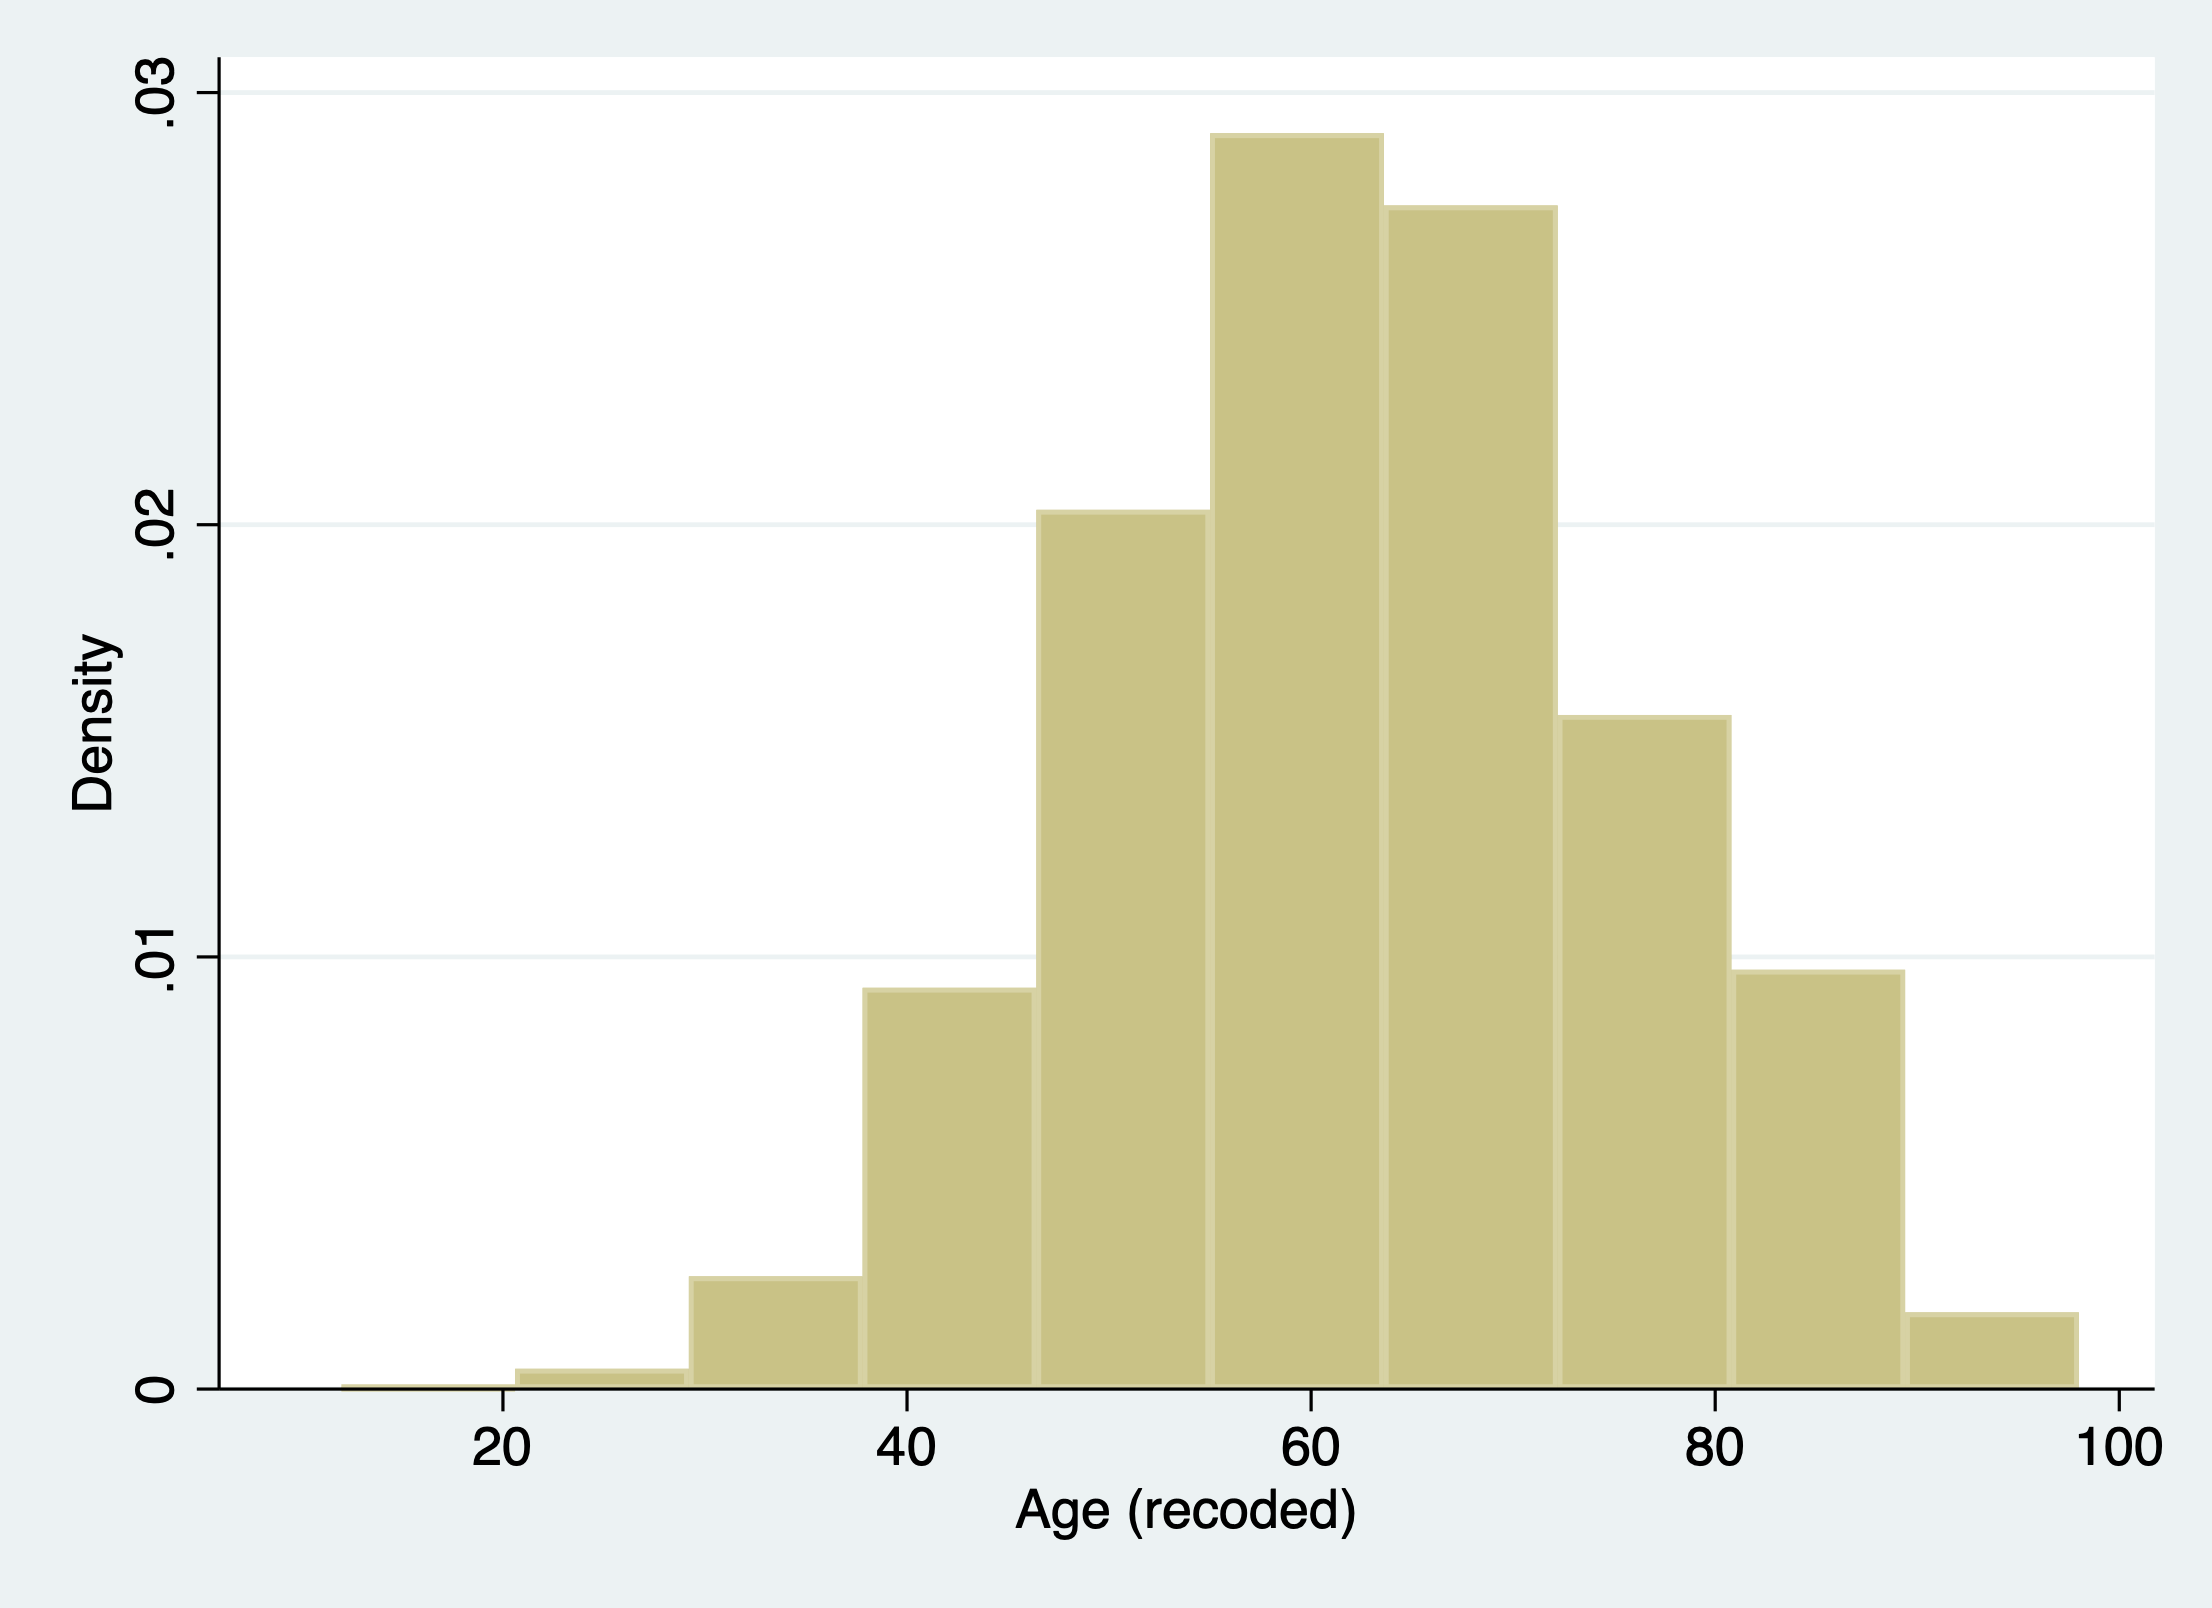
\includegraphics{images/histogram_stata2.png}

\hypertarget{boxplot2}{%
\paragraph*{Box plots}\label{boxplot2}}
\addcontentsline{toc}{paragraph}{Box plots}

Let's try making a boxplot of age.

\begin{Shaded}
\begin{Highlighting}[]
\KeywordTok{graph}\NormalTok{ box age}
\end{Highlighting}
\end{Shaded}

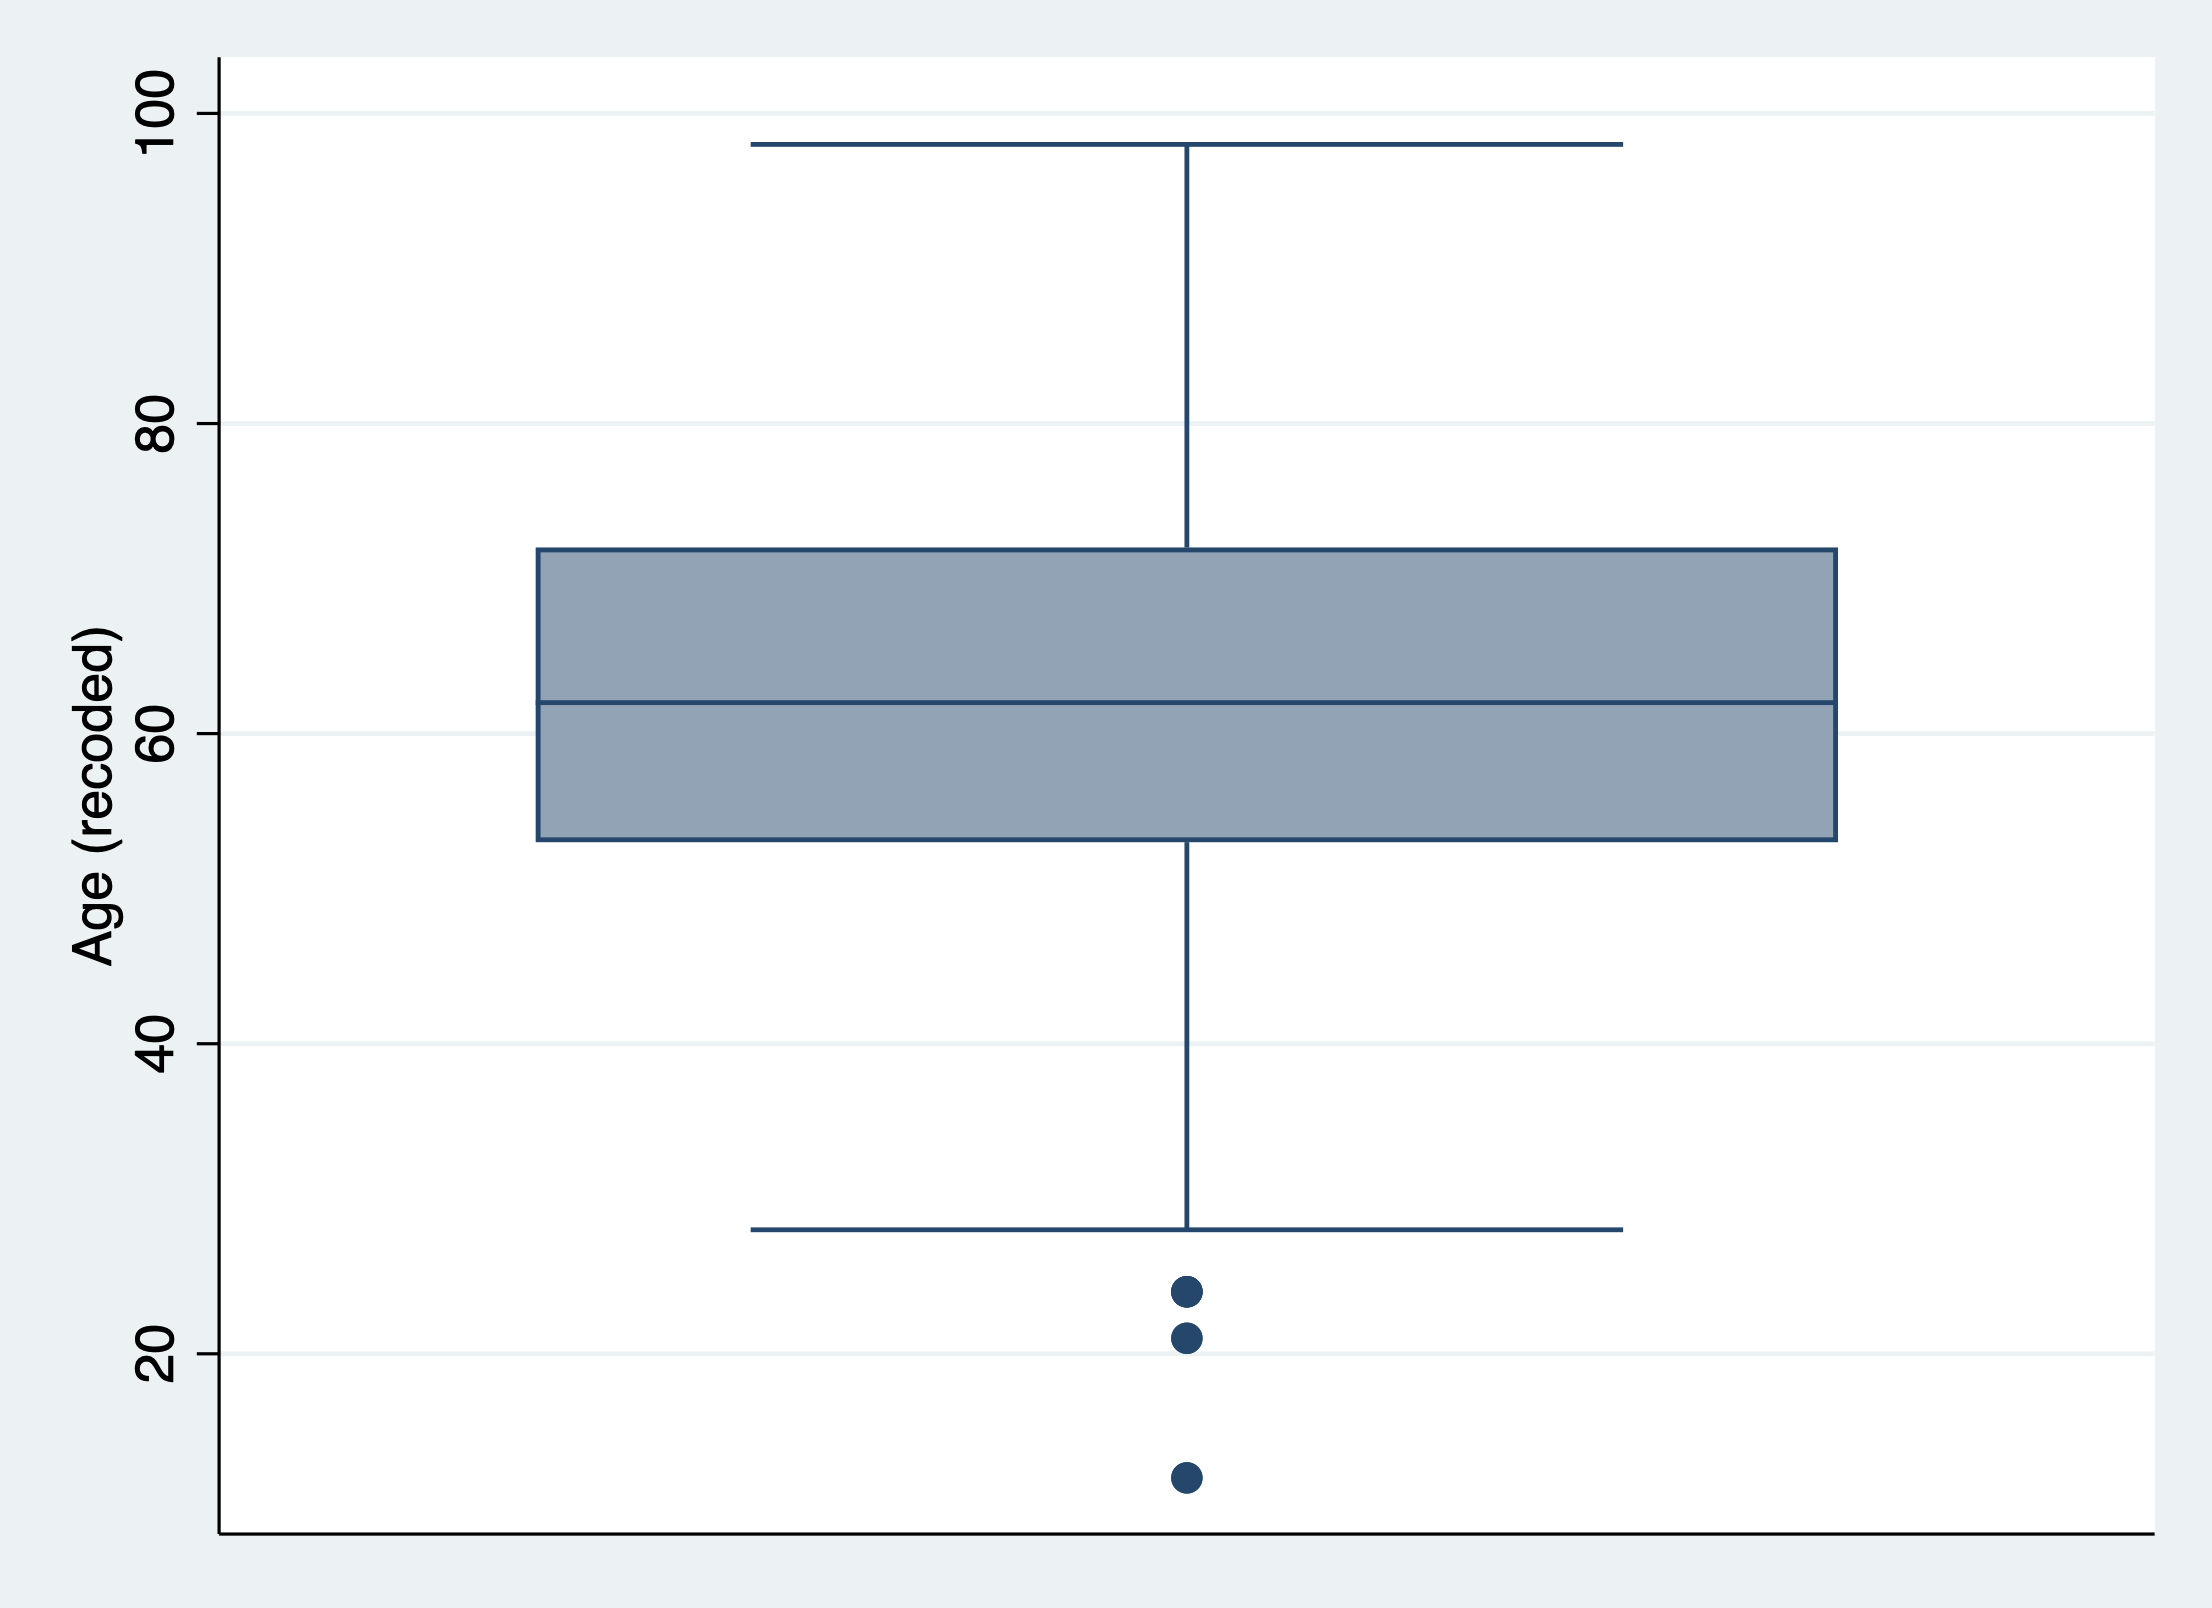
\includegraphics{images/box_stata.png}

Let's try making a boxplot of age by gender.

\begin{Shaded}
\begin{Highlighting}[]
\KeywordTok{graph}\NormalTok{ box age, }\BaseNTok{over}\NormalTok{(female2)}
\end{Highlighting}
\end{Shaded}

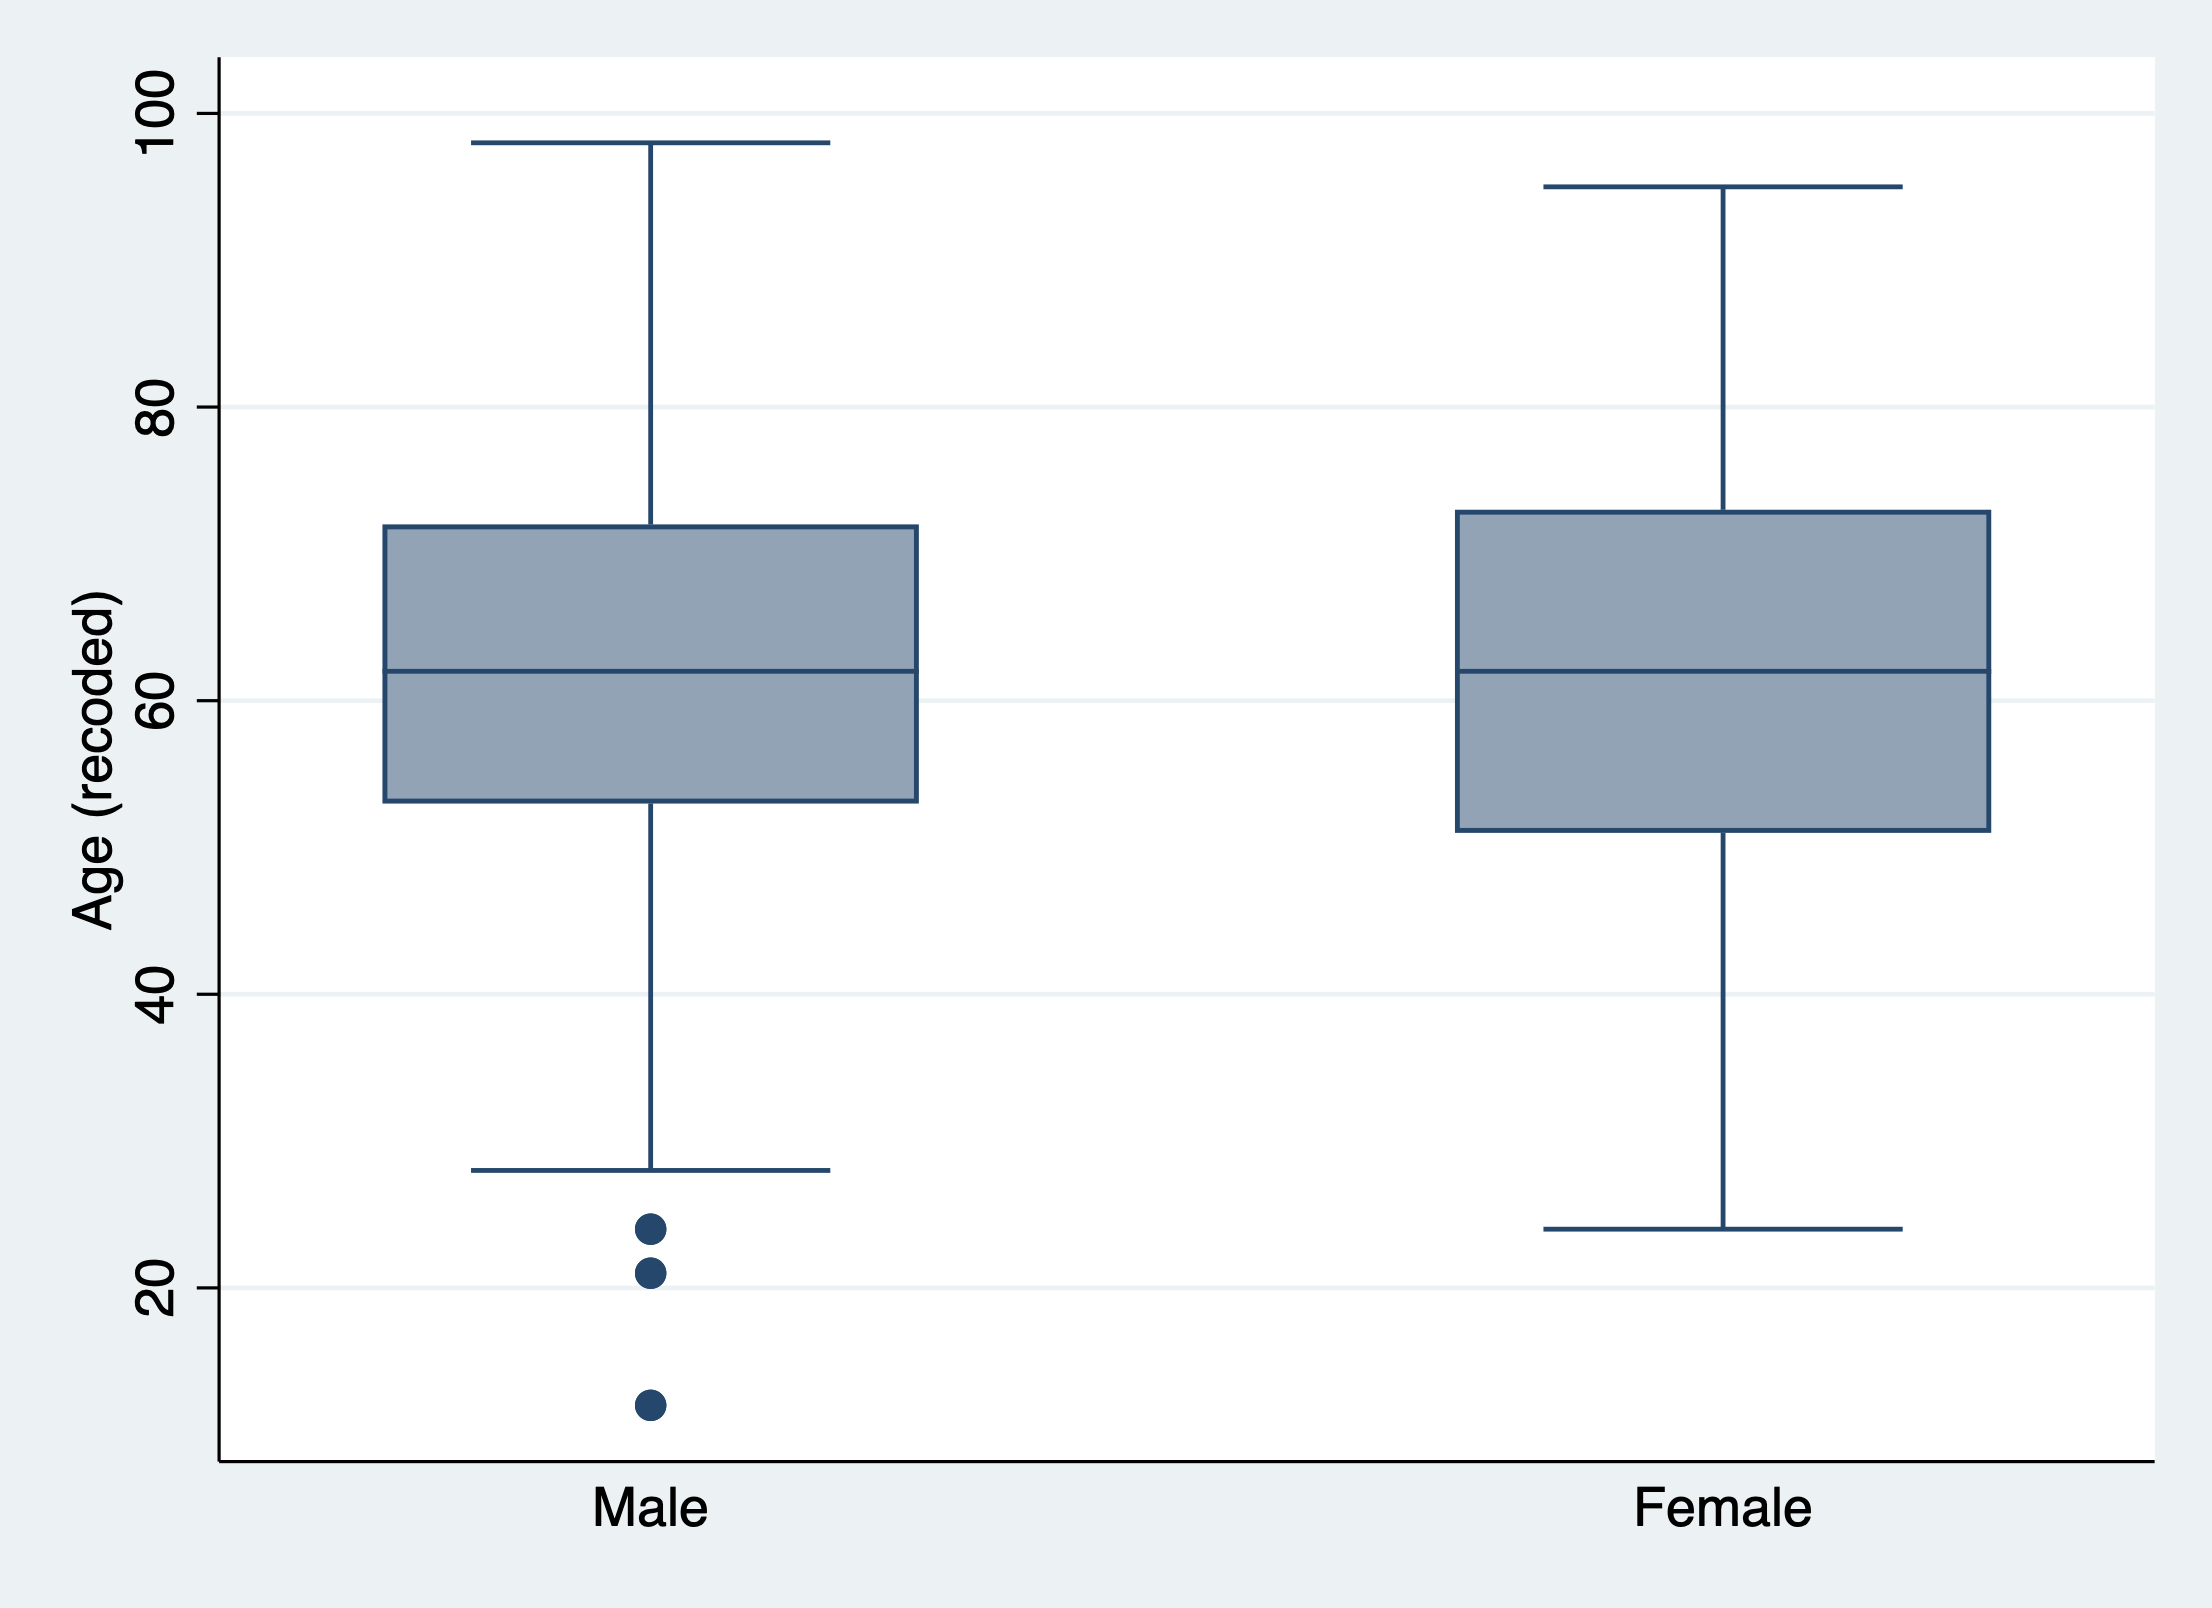
\includegraphics{images/boxover_stata.png}

\hypertarget{categorical-variables}{%
\subsubsection*{Categorical Variables}\label{categorical-variables}}
\addcontentsline{toc}{subsubsection}{Categorical Variables}

Again frequency tables are great, but sometimes a visualization of a categorical data can better communicate patterns.
\#\#\#\# Bar plots \{- \#barplot2\}

\begin{Shaded}
\begin{Highlighting}[]
\KeywordTok{graph} \BaseNTok{bar}\NormalTok{, }\BaseNTok{over}\NormalTok{ (female)}
\end{Highlighting}
\end{Shaded}

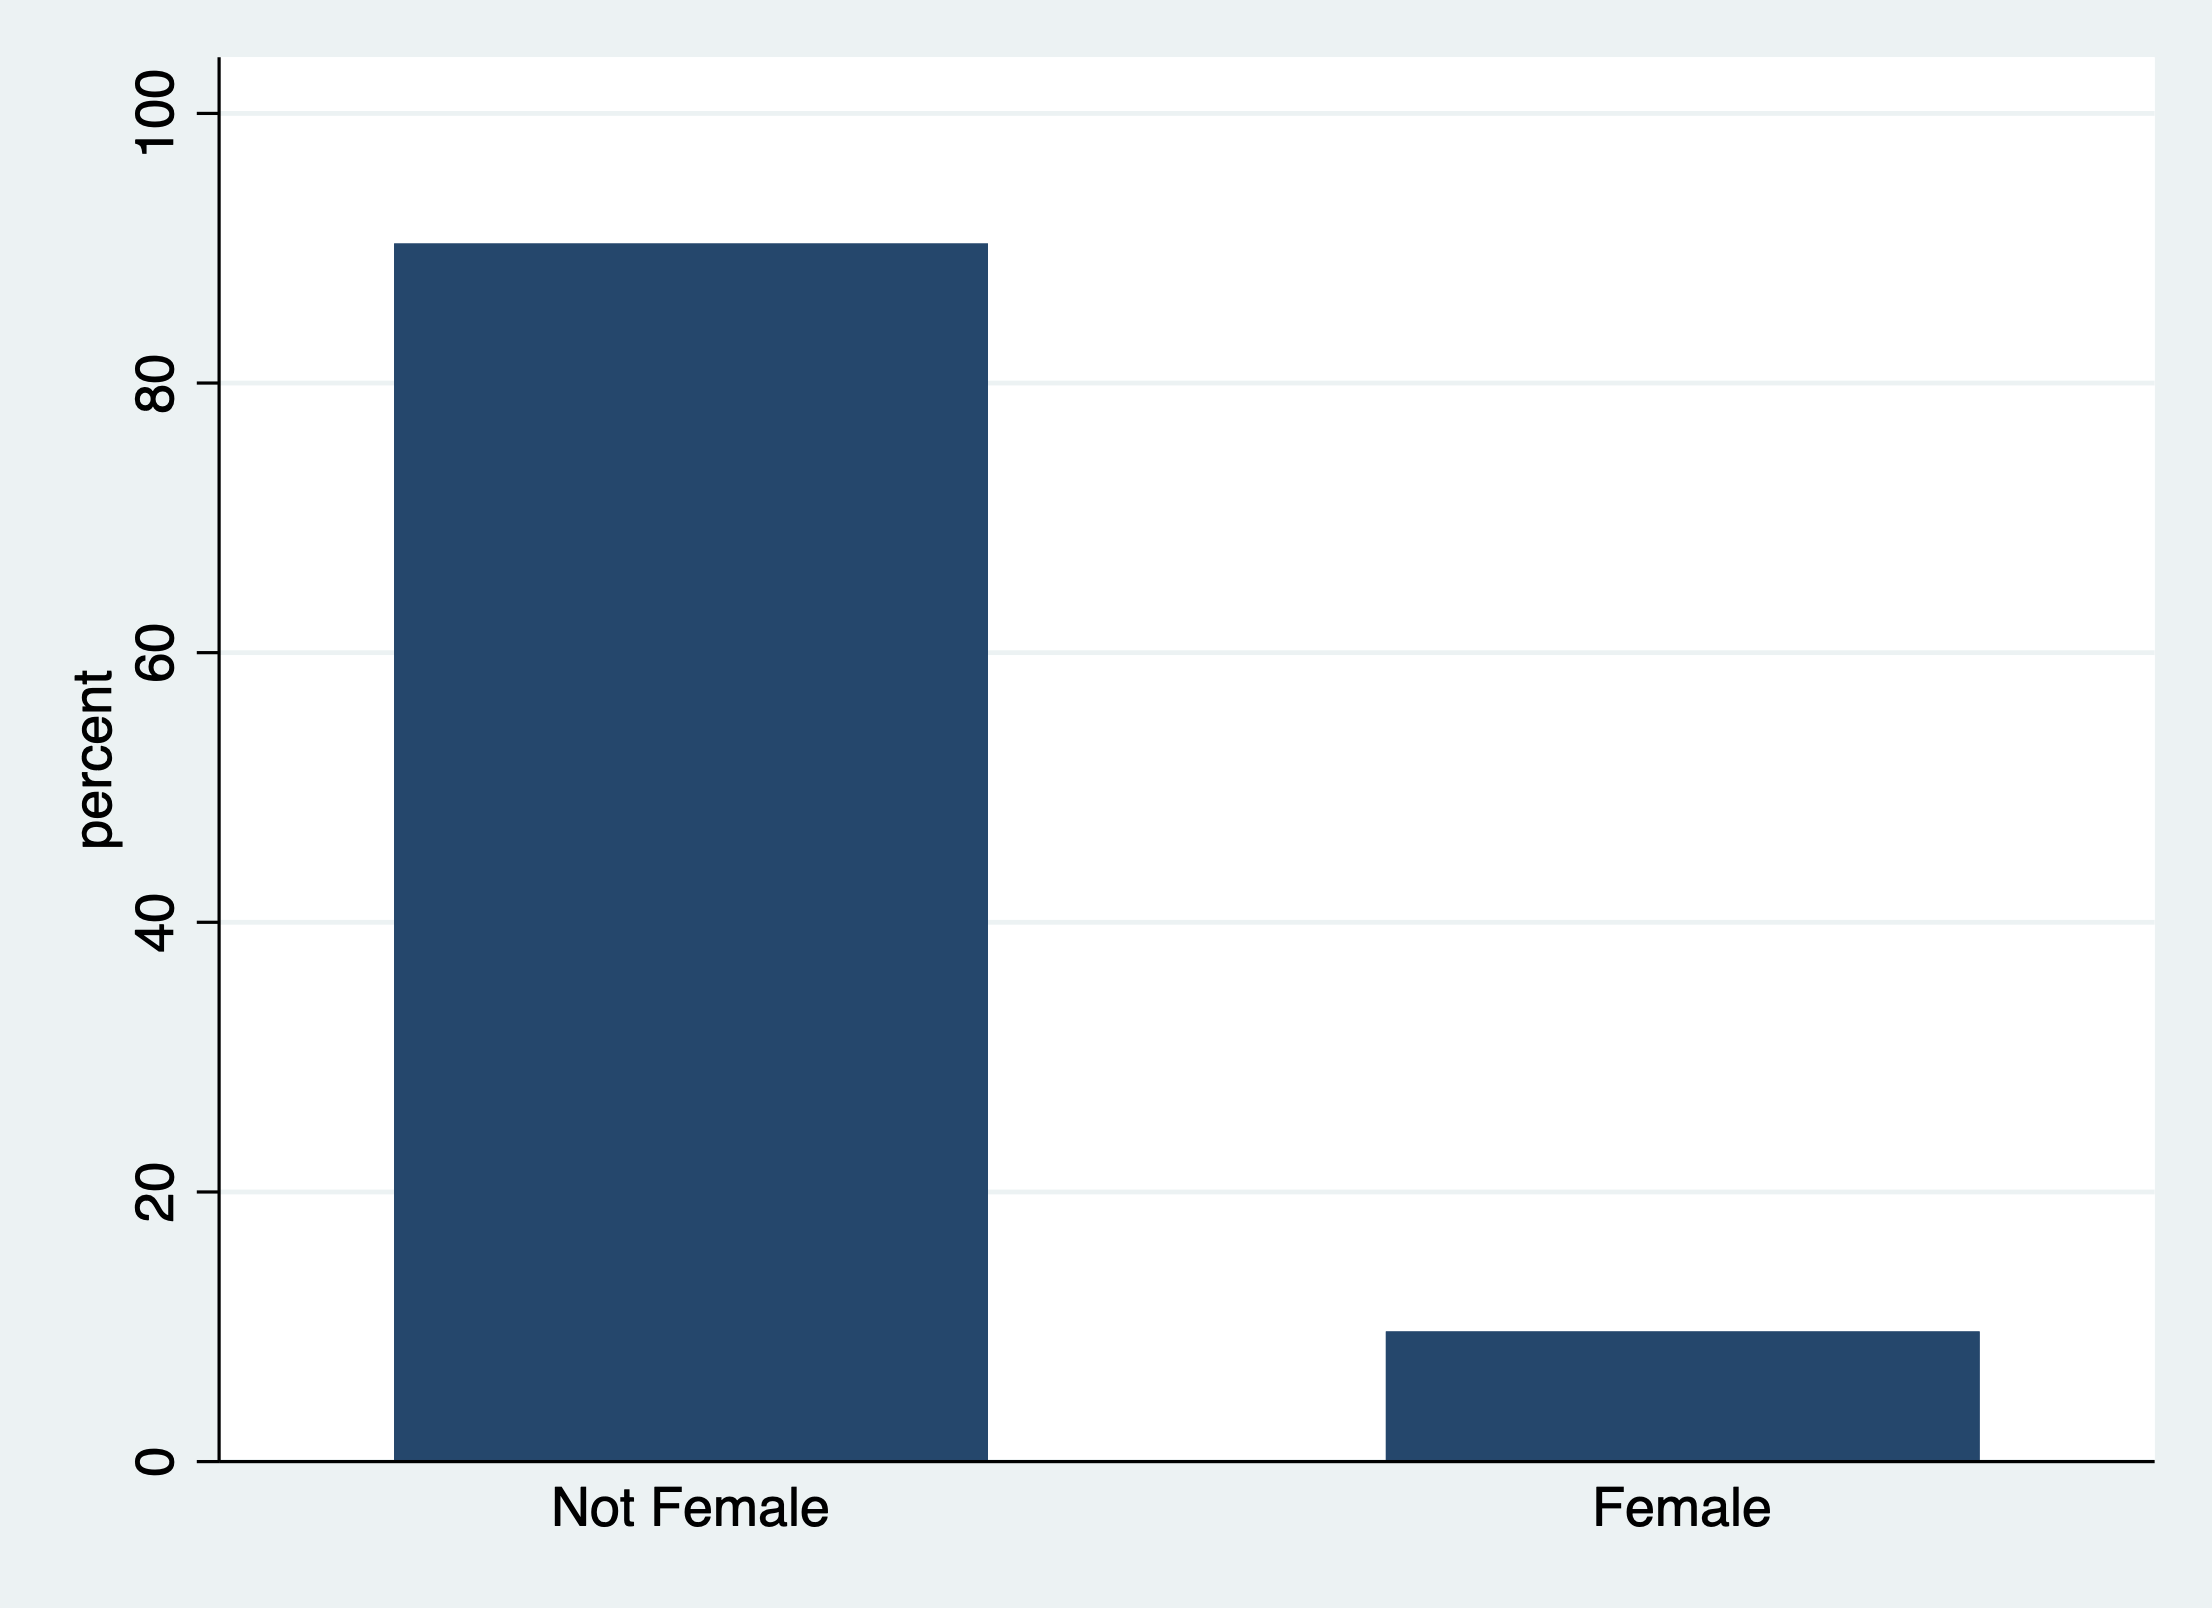
\includegraphics{images/bar_stata.png}

\hypertarget{subsetting-and-saving-data}{%
\subsection*{Subsetting and saving data}\label{subsetting-and-saving-data}}
\addcontentsline{toc}{subsection}{Subsetting and saving data}

Sometimes you'll be working with a huge dataset, and it is easier and cleaner save portion of observations and/or variables in a new dataset. This is called a sub-sample.

\hypertarget{keep}{%
\subsubsection*{Subset your data to specific variables}\label{keep}}
\addcontentsline{toc}{subsubsection}{Subset your data to specific variables}

Let's say you only want to keep the following three variables: year and the two variables you just created: age and female. For this task, you can use the \texttt{keep} command. We'll check it with the \texttt{describe} command.

\begin{Shaded}
\begin{Highlighting}[]
\KeywordTok{keep} \FunctionTok{year}\NormalTok{ age female2}
\KeywordTok{describe}
\end{Highlighting}
\end{Shaded}

\begin{verbatim}
Contains data from data_raw/SOC401_W21_Billionaires.dta
 Observations:         2,614                  
    Variables:             3                  9 Jan 2021 15:56
----------------------------------------------------------------------------------
Variable      Storage   Display    Value
    name         type    format    label      Variable label
----------------------------------------------------------------------------------
year            int     %8.0g                 
female2         float   %9.0g      gender2    Female (Male/Female)
age             float   %9.0g                 Age (recoded)
----------------------------------------------------------------------------------
Sorted by: 
     Note: Dataset has changed since last saved.
\end{verbatim}

You can also use the \texttt{drop} command if you only want to exclude a variable or two.

\begin{Shaded}
\begin{Highlighting}[]
\KeywordTok{drop}\NormalTok{ female2}
\end{Highlighting}
\end{Shaded}

\hypertarget{dropif}{%
\subsubsection*{Subset your data to specific observations}\label{dropif}}
\addcontentsline{toc}{subsubsection}{Subset your data to specific observations}

But what if you wanted to subset the data to only billionaires 30 or older? For this you can also use the \texttt{drop} command with an \texttt{if} conditional statement added. We'll check it with \texttt{summarize}.

\begin{Shaded}
\begin{Highlighting}[]
\KeywordTok{drop} \KeywordTok{if}\NormalTok{ age \textless{} 30 }
\KeywordTok{summarize}\NormalTok{ age }
\end{Highlighting}
\end{Shaded}

\begin{verbatim}
(10 observations deleted)

    Variable |        Obs        Mean    Std. dev.       Min        Max
-------------+---------------------------------------------------------
         age |      2,219    62.74448    12.91838         30         98
\end{verbatim}

\hypertarget{saving}{%
\subsubsection*{Saving your subset}\label{saving}}
\addcontentsline{toc}{subsubsection}{Saving your subset}

Now that you have your subset, you'll want to save it. Saving in Stata's data, format is simple. You add the \texttt{,\ replace} for when you are rurunning this .do file. If there is already a dataset named \texttt{mysubset.dta}, then stata will save over it with your new changes. \textbf{Take care} with saving over datasets. The action cannot be undone.

\begin{Shaded}
\begin{Highlighting}[]
\KeywordTok{save} \StringTok{"data\_work/mysubset.dta"}\NormalTok{, }\KeywordTok{replace}
\end{Highlighting}
\end{Shaded}

There are extra steps to save it other formats. .CSV files, are one of the most common formats you'll receive and save data in outside of Stata.

\begin{Shaded}
\begin{Highlighting}[]
\KeywordTok{export}\NormalTok{ delimited }\KeywordTok{using}\NormalTok{ data\_work/mysubset.csv, }\KeywordTok{replace} 
\end{Highlighting}
\end{Shaded}

\textbf{Remember}, every time you run these command it writes over your previous save. So be careful about version control and \textbf{ALWAYS} maintain the raw data file in a separate location.

\hypertarget{the-importance-of-annotation-and-clean-code}{%
\section{The Importance of Annotation and Clean Code}\label{the-importance-of-annotation-and-clean-code}}

A do file (aka a script) is not just a functional document where you conduct your analysis. It is also an important record of your analysis. When you read back through your do files you should be able to understand what each step of code is doing and why. Well-written code scripts:

\begin{itemize}
\tightlist
\item
  Have a header with your name and a title or a short description of what the script contains (e.g., ``Cleaning data for regression analysis on billionaires'')
\item
  Document the analytic decisions made about cleaning and analysis
\item
  Can be run from start to finish without errors
\end{itemize}

You may think that you will remember what you were thinking when you wrote a script, but sometimes you'll have to step away from an analysis for weeks or months. When you come back to it, your notes will remind you exactly why you coded things the way you did. Your code scripts will also be read by other people. It may be collaborators, advisers, or colleagues who agree to quality check your code to look for errors. It is also more and more common for journals to ask scholars to post their coding files so that other people can replicate your analysis.

\hypertarget{how-to-make-notes-in-your-script}{%
\subsection*{How to make notes in your script}\label{how-to-make-notes-in-your-script}}
\addcontentsline{toc}{subsection}{How to make notes in your script}

The main way to make a note in an Stata .do script is to use the \texttt{*} at the beginning of a line.

Let's return to our code to subset our data to billionaires 30 or older. In this code I note above the command what it is about to do. In the second command, I include a note one the same line to remind myself that I want to check to make sure the code I ran worked correctly.
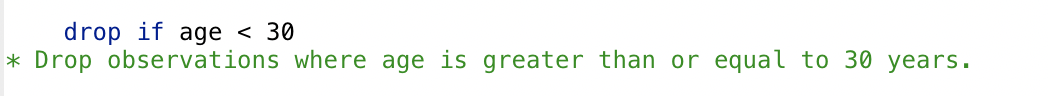
\includegraphics[width=5.20833in,height=\textheight]{images/notes1.png}

You can also use \texttt{/*\ */} to create notes that span across multiple lines. For example:
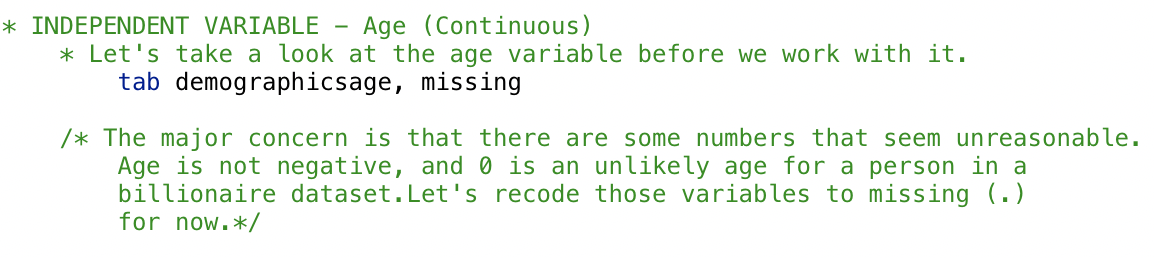
\includegraphics[width=5.20833in,height=\textheight]{images/notes2.png}
If you want to add a note to the end of a command you can put a double slash \texttt{//}

\includegraphics[width=5.20833in,height=\textheight]{images/notes3.png}

\hypertarget{tips-for-neat-code}{%
\subsection*{Tips for Neat Code}\label{tips-for-neat-code}}
\addcontentsline{toc}{subsection}{Tips for Neat Code}

Notes are a huge part of making your code readable to yourself and others. However, writing neat code is also an enormous gift you can give to yourself, to the TA grading your do files, and anyone else trying to make sense of your code. Here are my top tips for writing neat code in Stata:

\begin{itemize}
\tightlist
\item
  Split long functions and commands across multiple lines
\item
  Leave spaces around equals signs and other operators
\item
  Create headers and sections in your code
\item
  Create clear names for your variables
\end{itemize}

\hypertarget{split-long-functions-and-commands-across-multiple-lines}{%
\subsubsection*{Split long functions and commands across multiple lines}\label{split-long-functions-and-commands-across-multiple-lines}}
\addcontentsline{toc}{subsubsection}{Split long functions and commands across multiple lines}

Nothing, I repeat, nothing makes code harder to read than shoving it all into one long line. It can be a little tricky to split some commands across multiple lines in Stata, but it is possible and makes your code much cleaner. You can do so by adding a triple forward slash to the end of a line (\texttt{///}). This tells stata that the command continues on the next line. You can use this over as many lines as you want.

Take this example. Say we wanted to keep many variables in our subset.

\begin{Shaded}
\begin{Highlighting}[]
\KeywordTok{keep}\NormalTok{ wealthworthinbillions demographicsage demographicsgender2 wealthhowinherited2 wealthtype2 wealthhowcategory2 locationregion2}
\end{Highlighting}
\end{Shaded}

These lines of code will run just fine, but they are difficult for your eye to parse when squished together. Let your code breathe!

\begin{Shaded}
\begin{Highlighting}[]
\NormalTok{keep wealthworthinbillions demographicsage demographicsgender2 }\SpecialCharTok{/}\ErrorTok{//}
\NormalTok{  wealthhowinherited2 wealthtype2 wealthhowcategory2 locationregion2}
\end{Highlighting}
\end{Shaded}

As a rule, don't let any line get past about 80 characters. Stata .do files include a
vertical line at about this point. I recommend that you don't write past it in
your code scripts. It will help you and the reader avoid the annoying horizontal scroll bar.

\hypertarget{leave-spaces-around-operators}{%
\subsubsection*{Leave spaces around operators}\label{leave-spaces-around-operators}}
\addcontentsline{toc}{subsubsection}{Leave spaces around operators}

This is another tip to let your code breathe! When coding it is best practice to
put a space after any comma or logical operator. Take the line of code below:

\begin{Shaded}
\begin{Highlighting}[]
\KeywordTok{replace}\NormalTok{ female2=0 }\KeywordTok{if}\NormalTok{ demographicsgender2==2 | demographicsgender2==3}
\KeywordTok{replace}\NormalTok{ female2=1 }\KeywordTok{if}\NormalTok{ demographicsgender2==1}
\end{Highlighting}
\end{Shaded}

It works, but it's cluttered and makes it difficult to read. Take a look at this
line in a cleaner format:

\begin{Shaded}
\begin{Highlighting}[]
\NormalTok{replace female2 }\OtherTok{=} \DecValTok{0} \ControlFlowTok{if}\NormalTok{ demographicsgender2 }\SpecialCharTok{==} \DecValTok{2} \SpecialCharTok{|}\NormalTok{ demographicsgender2 }\SpecialCharTok{==} \DecValTok{3}
\NormalTok{replace female2 }\OtherTok{=} \DecValTok{1} \ControlFlowTok{if}\NormalTok{ demographicsgender2 }\SpecialCharTok{==} \DecValTok{1}
\end{Highlighting}
\end{Shaded}

Notice how I've added a space on both sides of the equals signs. This makes it easier to understand and edit your code.

\hypertarget{create-headers-and-sections-in-your-code}{%
\subsubsection*{Create headers and sections in your code}\label{create-headers-and-sections-in-your-code}}
\addcontentsline{toc}{subsubsection}{Create headers and sections in your code}

You wouldn't write a paper without any titles or sections, so don't write your code without titles or sections! Take a look back at the Stata do script for this lab. Notice how I put a section header for setting up your environment, exploring your data, cleaning your data, and so on. Hopefully this made it easier for you to work through the script.

\hypertarget{create-clear-names-for-your-variables}{%
\subsubsection*{Create clear names for your variables}\label{create-clear-names-for-your-variables}}
\addcontentsline{toc}{subsubsection}{Create clear names for your variables}

Everyone has their own preferred naming system for variables and data sets. The golden rule for naming is consistency. For example, if I recode variables I will often add \texttt{\_rc} to the end for recode (e.g., \texttt{age} and \texttt{age\_rc}). Other tips:

\begin{itemize}
\tightlist
\item
  Make your names explicit, but brief (e.g., \texttt{billionaires\_over30.dta})
\item
  Don't include spaces in your file names, it makes file paths difficult
\end{itemize}

\hypertarget{activity}{%
\section{Activity}\label{activity}}

For this class, we expect you to write legible, clean code. To kick start this process, I want you to begin develop your own coding style. By class on Monday, email me (\texttt{rosewerth@u.northwestern.edu}) a script file for a hypothetical data cleaning script. The script should include:

\begin{enumerate}
\def\labelenumi{\arabic{enumi})}
\tightlist
\item
  A script header with your name, the date you created the script, and a short description of what the script contains
\item
  Two section headers
\item
  A command to set your working directory to the main folder you created in this lab
\item
  A note telling me what you find easy about coding in Stata and what you find difficult about coding in Stata.
\end{enumerate}

This should be your template for writing clean scripts for the rest of the quarter. Your template can evolve, but I expect all your scripts moving forward to contain title and section headers and clear annotation for each step in your code.

\hypertarget{lab-1-r}{%
\chapter{Lab 1 (R)}\label{lab-1-r}}

\hypertarget{lab-goals-instructions-1}{%
\section{Lab Goals \& Instructions}\label{lab-goals-instructions-1}}

\begin{itemize}
\tightlist
\item
  Review the basics of data cleaning\\
\item
  Learn the importance of annotating code
\item
  Start develop your own coding style
\end{itemize}

\textbf{Instructions}

\begin{enumerate}
\def\labelenumi{\arabic{enumi}.}
\tightlist
\item
  Download the data file (\texttt{SOC401\_W21\_Billionaires.rda}) and R script (\texttt{401-1-Lab1.R}) from the links below.
\item
  Create a project following \protect\hyperlink{project}{the instructions in 3.3 below}
\item
  Work through the R script, executing each line of code. This page contains the same material, with more explanation about the functions used.
\item
  Read through the Importance of \protect\hyperlink{annotate}{Annotation and Clean Code}, and complete the short activity at the bottom of the page. Email the .R script file to me by class on Monday.
\end{enumerate}

\textbf{Jump Links to Functions in this Lab:}\\
\protect\hyperlink{global}{Global view of dataset}\\
\protect\hyperlink{names}{List of variable names}\\
\protect\hyperlink{head}{First 10 rows of data set or variable values}\\
\protect\hyperlink{missing}{Missing observations}\\
\protect\hyperlink{descriptive}{Descriptive statistics}\\
\protect\hyperlink{frequency}{Frequency tables}\\
\protect\hyperlink{mutate}{mutate}\\
\protect\hyperlink{ifelse}{ifelse}\\
\protect\hyperlink{hist}{Histogram with base R}\\
\protect\hyperlink{histgg}{Histogram with ggplot}\\
\protect\hyperlink{boxplot}{Boxplot with ggplot}
\protect\hyperlink{barplot}{Bar plot with ggplot}
\protect\hyperlink{select}{select}\\
\protect\hyperlink{filter}{filter}\\
\protect\hyperlink{save}{Save data files}

\hypertarget{lab-files-1}{%
\section{Lab Files}\label{lab-files-1}}

\hypertarget{project}{%
\section{Create a Project}\label{project}}

In R, it is always best to work within what is called a ``Project'' when you are coding and analyzing data. Life can get messy and so can data analysis. Creating a project and a file structure is the equivalent of keeping a clean work space. You may not mind a messy desk, but a messy file structure will be a nightmare for your collaborators and increase your risk of making mistakes in your analysis. With quantitative data analysis, file management is crucial.
RStudio has created a wonderful project management tool for you. It's an umbrella file that organizes all your scripts, folders, figures, and more. It also sets your working directory for you, which we will \protect\hyperlink{environment}{discuss more below}.

For your first task, create a project in R for this class.

\begin{enumerate}
\def\labelenumi{\arabic{enumi}.}
\tightlist
\item
  Open RStudio.
\item
  Click the ``File'' menu button, then ``New Project''.
\item
  Click ``New Directory''.
\item
  Click ``New Project''.
\item
  Type in the name of the directory to store your project, e.g.~``401-1\_Linear Regression''. Make sure you choose the parent folder on your computer where you want these files to be stored. Your project will live in new folder with the name you gave your directory. Your project and all your files will be stored there.
\item
  Click the ``Create Project'' button.
\end{enumerate}

Now let's make sure you can open this project, create a file folder structure, and move your lab files for today into the appropriate spot.

\begin{enumerate}
\def\labelenumi{\arabic{enumi}.}
\tightlist
\item
  Exit RStudio
\item
  Navigate to the folder where you created your directory. Double click on the \texttt{.Rproj} file you created.\\
\item
  Open up a blank R script and use the following code to create a file structure.
\end{enumerate}

\begin{Shaded}
\begin{Highlighting}[]
\FunctionTok{dir.create}\NormalTok{(}\StringTok{"data\_raw"}\NormalTok{)}
\FunctionTok{dir.create}\NormalTok{(}\StringTok{"data\_work"}\NormalTok{)}
\FunctionTok{dir.create}\NormalTok{(}\StringTok{"fig\_output"}\NormalTok{)}
\FunctionTok{dir.create}\NormalTok{(}\StringTok{"scripts"}\NormalTok{)}
\end{Highlighting}
\end{Shaded}

\begin{enumerate}
\def\labelenumi{\arabic{enumi}.}
\setcounter{enumi}{3}
\tightlist
\item
  Move \texttt{SOC401\_W21\_Billionaires.rda} to your \texttt{data\_raw} folder.
\item
  Move \texttt{401-1-Lab1.R} to your \texttt{scripts} folder.
\end{enumerate}

For more information on best data management practices, and to see the source of some of the instructions above \href{https://swcarpentry.github.io/r-novice-gapminder/02-project-intro/index.html}{check out this R tutorial}.

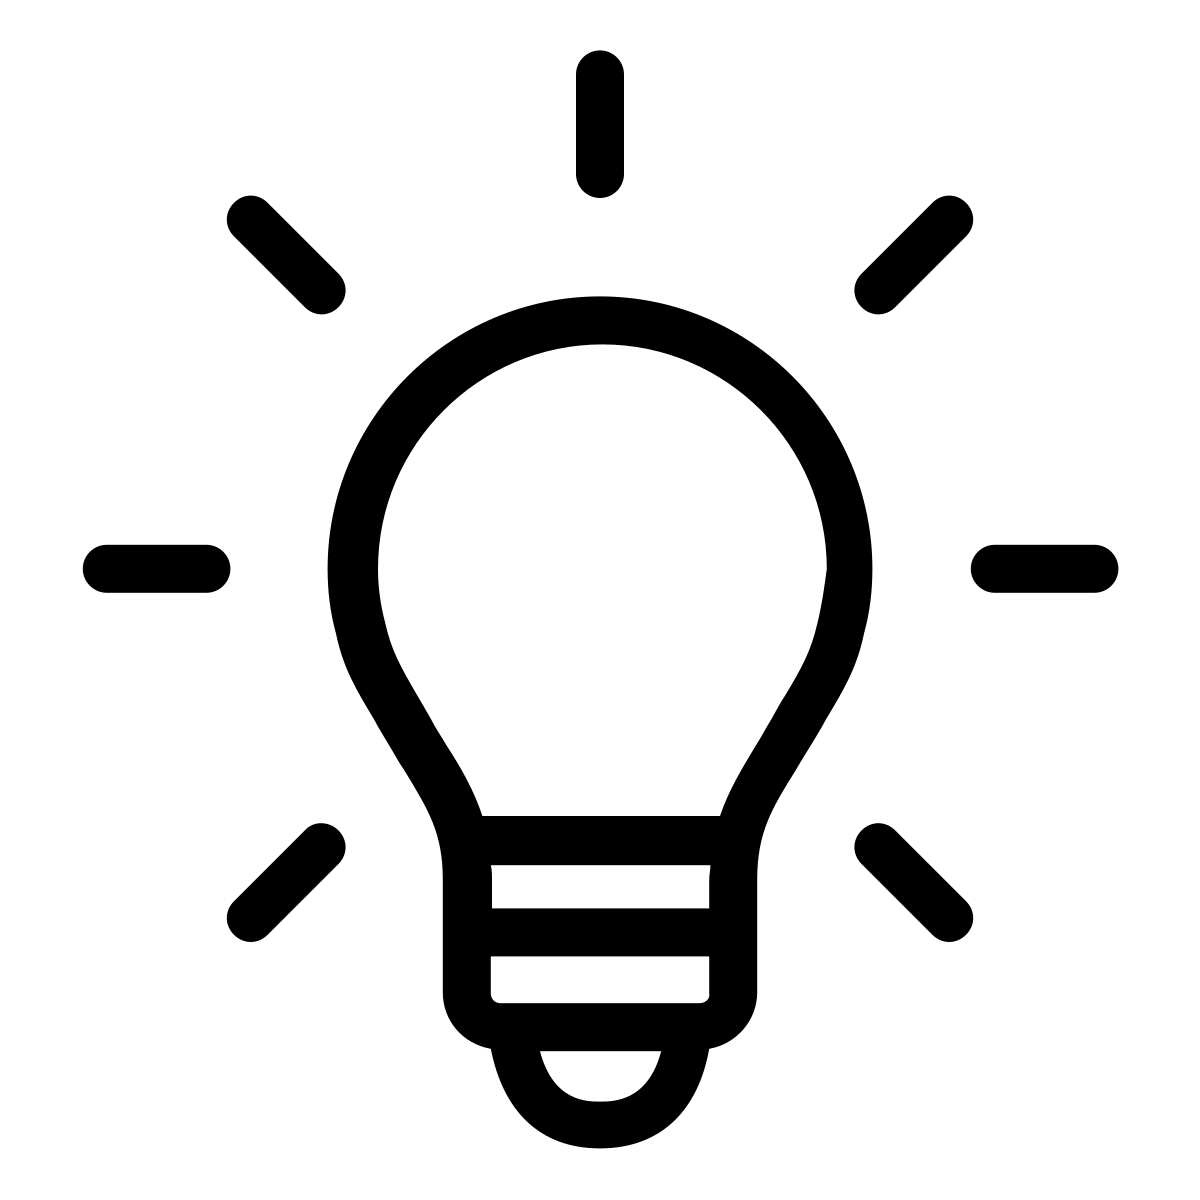
\includegraphics[width=0.36458in,height=\textheight]{images/bulb.png} Data Tip

\begin{quote}
Why do I need two separate folders for data?\\
You should aways store your original, raw data files in a place where they are in no danger of being saved over, altered, or lost. One great way of protecting your original data files is to create two folders for data: one folder for your raw files and one folder where you can saved cleaned datasets and subsets.
\end{quote}

\hypertarget{data-cleaning-1}{%
\section{Data Cleaning}\label{data-cleaning-1}}

95 percent of the work of quantitative research is getting your data in shape to run your model. This tutorial assumes that you have R downloaded and are familiar with the basics of the language. If you are not, here are some resources to help you get started coding in R.

\begin{itemize}
\tightlist
\item
  \href{https://r4ds.had.co.nz/}{R for Data Science}. A great online book to help you learn R on your own.
\item
  \href{https://www.youtube.com/playlist?list=PL6gx4Cwl9DGCzVMGCPi1kwvABu7eWv08P}{R Programming Tutorials on Youtube}
\item
  \href{https://www.r-bloggers.com/2021/04/tidyverse-in-r-complete-tutorial/}{A quick tutorial for the Tidyverse}. The tidyverse makes datacleaning in R a much simpler process.
\item
  \href{https://ggplot2-book.org/index.html}{A great book on ggplot2}. ggplot2 is the best package for making graphs in any software.
\end{itemize}

Northwestern's Research Computing Services \href{https://www.it.northwestern.edu/research/training.html}{offers great trainings in a variety of software languages}, including R, on a regular basis. Check them out and get on their email list.

\hypertarget{environment}{%
\subsection*{Set up the environment}\label{environment}}
\addcontentsline{toc}{subsection}{Set up the environment}

Before you get to work cleaning your data, you need to let the software know where to grab and save your files. This saves you from having to type in a long file path anytime you want to do something. If you are working in a project, you are good to go! Not sure if you are working in your project? If you look in the top right corner of your RStudio window, you should see the name of you project next to the project icon. If you see ``None'' or a different name, that means you need to open your project and start working from there!
If you are not working in a project, you should begin your file by setting your working directory. Your working directory is the folder on your computer where you want to store all your data and script files. Below you will see the path to my working directory. You should replace the filepath with the one you want to use.

\begin{Shaded}
\begin{Highlighting}[]
\CommentTok{\# Set your working directory }
\FunctionTok{setwd}\NormalTok{(}\StringTok{"\textasciitilde{}/Documents/Work \& Research/Regression Labs"}\NormalTok{)}
\end{Highlighting}
\end{Shaded}

\textbf{Load your libraries}\\
When you are cleaning datasets these are the basic packages that are useful. Make sure you load them before beginning work.

\begin{Shaded}
\begin{Highlighting}[]
\FunctionTok{library}\NormalTok{(tidyverse)}
\FunctionTok{library}\NormalTok{(dplyr)}
\FunctionTok{library}\NormalTok{(janitor)}
\FunctionTok{library}\NormalTok{(ggplot2)}
\FunctionTok{library}\NormalTok{(skimr)}
\FunctionTok{library}\NormalTok{(pillar)}
\end{Highlighting}
\end{Shaded}

\begin{verbatim}
Attaching package: 'kableExtra'
\end{verbatim}

\begin{verbatim}
The following object is masked from 'package:dplyr':

    group_rows
\end{verbatim}

Note: if you do not have one of these packages installed, you will need to first install it using the command: \texttt{install.packages("skimr")}

\textbf{Load your data}\\
Now that you've set your working directory, you can tell R to go grab your data and load it into your working environment.
Loading data that is in R's data formats is easy. An R data file ends in .rda or .rData.

\begin{Shaded}
\begin{Highlighting}[]
\FunctionTok{load}\NormalTok{(}\StringTok{"data\_raw/SOC401\_W21\_Billionaires.rda"}\NormalTok{)}
\end{Highlighting}
\end{Shaded}

You can also load data in other formats. Here are a few common ones.

\begin{Shaded}
\begin{Highlighting}[]
\CommentTok{\# Stata}
\FunctionTok{read\_dta}\NormalTok{(}\StringTok{"data\_raw/SOC401\_W21\_Billionaires.dta"}\NormalTok{)}

\CommentTok{\# CSV}
\FunctionTok{read.csv}\NormalTok{(}\StringTok{"data\_raw/SOC401\_W21\_Billionaires.csv"}\NormalTok{)}
\end{Highlighting}
\end{Shaded}

Check out this tutorial on how to load excel data:
\url{https://www.datacamp.com/community/tutorials/r-tutorial-read-excel-into-r}

At this point, it can also be helpful to rename your dataset to something short and easy to type. You are going to be typing it a lot in your R code.

\begin{Shaded}
\begin{Highlighting}[]
\NormalTok{mydata }\OtherTok{\textless{}{-}}\NormalTok{ SOC401\_W21\_Billionaires }\CommentTok{\# this saves the dataset as a new dataframe in our environment.}
\end{Highlighting}
\end{Shaded}

\hypertarget{exploring-your-data-1}{%
\subsection*{Exploring your data}\label{exploring-your-data-1}}
\addcontentsline{toc}{subsection}{Exploring your data}

When you begin any new project, it is important to understand the condition of your variables. Here are a few important functions you need to begin that process.

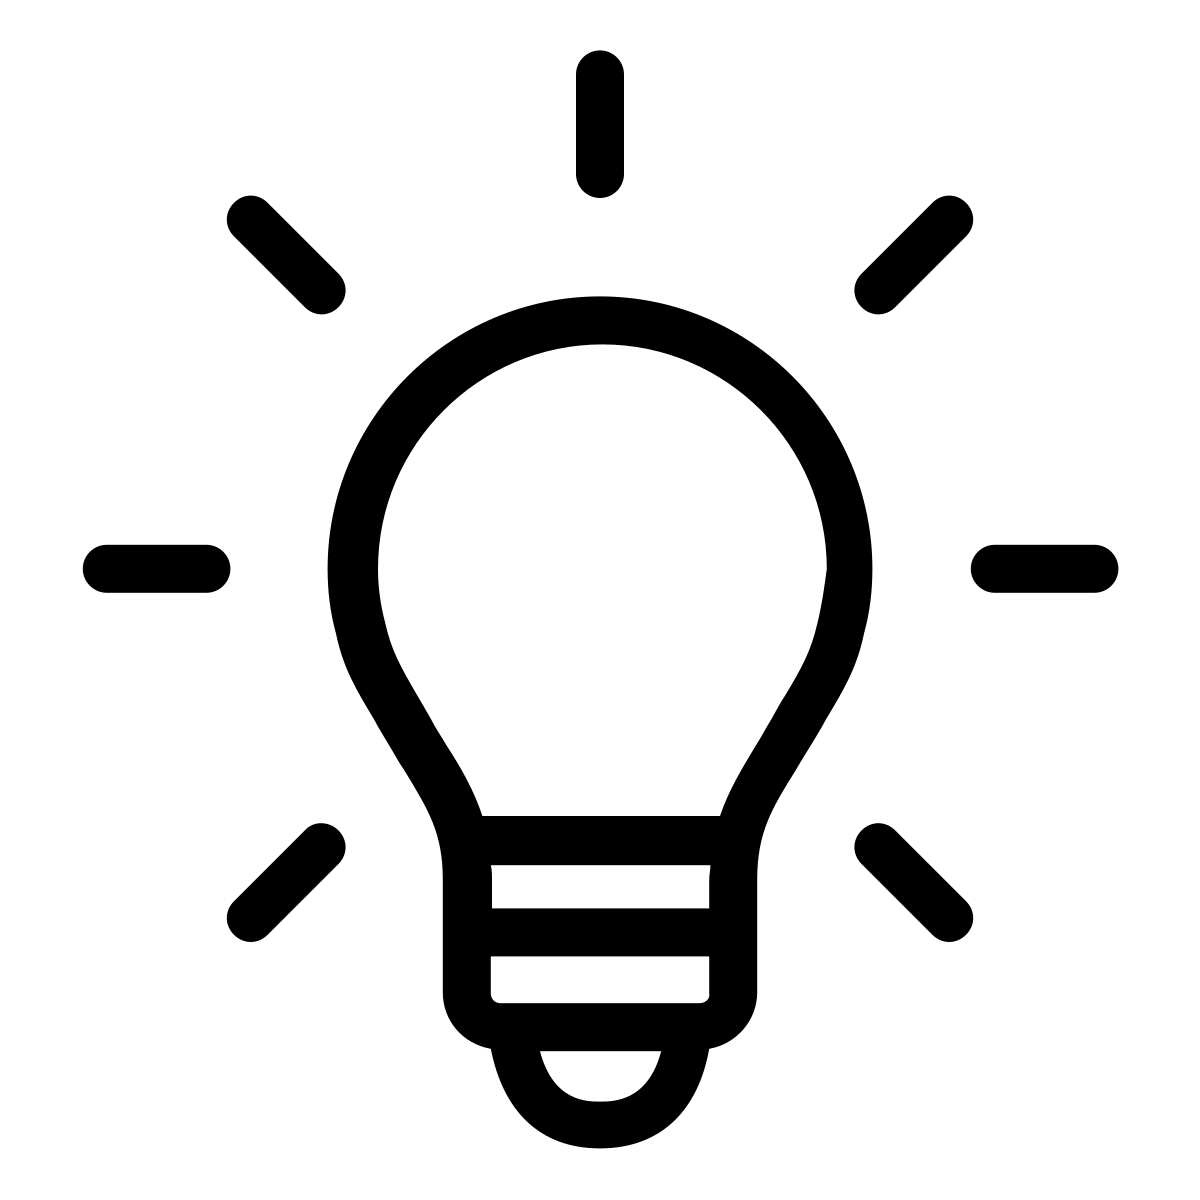
\includegraphics[width=0.36458in,height=\textheight]{images/bulb.png} Data Tip

\begin{quote}
Remember if this script or any other uses a function that you are not familiar with, you can search for the function online or type `?' and then the name of the function you want to look up in the console. For example, `?ifelse( )' will pull up the documentation for that function.
\end{quote}

\hypertarget{global}{%
\subsubsection*{Let's start by taking a global look at your dataset.}\label{global}}
\addcontentsline{toc}{subsubsection}{Let's start by taking a global look at your dataset.}

There are countless ways to do this, but I am providing you with two helpful functions from two different packages.

Option 1 from the \texttt{skimr} library:

\begin{Shaded}
\begin{Highlighting}[]
\FunctionTok{skim\_without\_charts}\NormalTok{(mydata)}
\end{Highlighting}
\end{Shaded}

\begin{verbatim}
Error in kable_latex(x = structure(c("Name", "Number of rows", "Number of columns", : unused argument (table.attr = "style='width: auto;'\n        class='table table-condensed'")
\end{verbatim}

The \texttt{skim\_without\_charts()} function does several great things. It includes the number of observations (rows) and variables (columnns), separates the variables by type (e.g., character vs.~numeric), it has a nice compact presentation format, and includes all your basic descriptive statistics.

Option 2 from the \texttt{pillar} library:

\begin{Shaded}
\begin{Highlighting}[]
\FunctionTok{glimpse}\NormalTok{(mydata)}
\end{Highlighting}
\end{Shaded}

\begin{verbatim}
Rows: 2,614
Columns: 21
$ name                  <chr> "Bill Gates", "Bill Gates", "Bill Gates", "Warre~
$ rank                  <dbl> 1, 1, 1, 2, 2, 2, 3, 3, 3, 4, 4, 4, 5, 5, 5, 6, ~
$ year                  <dbl> 1996, 2001, 2014, 1996, 2001, 2014, 1996, 2001, ~
$ companyfounded        <dbl> 1975, 1975, 1975, 1962, 1962, 1990, 1896, 1975, ~
$ companyname           <chr> "Microsoft", "Microsoft", "Microsoft", "Berkshir~
$ demographicsage       <dbl> 40, 45, 58, 65, 70, 74, 0, 48, 77, 68, 56, 83, 7~
$ locationgdp           <dbl> 8.10e+12, 1.06e+13, 0.00e+00, 8.10e+12, 1.06e+13~
$ wealthworthinbillions <dbl> 18.5, 58.7, 76.0, 15.0, 32.3, 72.0, 13.1, 30.4, ~
$ wealthhowfromemerging <chr> "True", "True", "True", "True", "True", "True", ~
$ wealthhowwasfounder   <chr> "True", "True", "True", "True", "True", "True", ~
$ wealthhowwaspolitical <chr> "True", "True", "True", "True", "True", "True", ~
$ wealthhowinherited2   <dbl> 5, 5, 5, 5, 5, 5, 1, 5, 5, 5, 5, 5, 5, 5, 5, 4, ~
$ wealthhowcategory2    <dbl> 4, 4, 4, 7, 7, 5, 4, 4, 5, 3, 4, 7, 3, 5, 4, 3, ~
$ wealthtype2           <dbl> 2, 2, 2, 2, 2, 4, 3, 2, 2, 5, 2, 2, 5, 2, 2, 3, ~
$ wealthhowindustry2    <dbl> 15, 15, 15, 3, 3, 7, 16, 15, 14, 13, 15, 3, 6, 1~
$ locationregion2       <dbl> 6, 6, 6, 6, 6, 4, 3, 6, 3, 2, 6, 6, 2, 3, 6, 2, ~
$ locationcountrycode2  <dbl> 71, 71, 71, 71, 71, 47, 11, 71, 23, 30, 71, 71, ~
$ locationcitizenship2  <dbl> 71, 71, 71, 71, 71, 39, 62, 71, 58, 25, 71, 71, ~
$ demographicsgender2   <dbl> 2, 2, 2, 2, 2, 2, NA, 2, 2, 2, 2, 2, 2, 2, 2, 2,~
$ companysector2        <dbl> 5, 5, 5, 3, 3, 2, 379, 466, 13, 402, 10, 3, 66, ~
$ companyrelationship2  <dbl> 32, 32, 32, 32, 32, 32, NA, 32, 32, 44, 32, 32, ~
\end{verbatim}

The \texttt{glimpse} function is not as compact as skim, but it also includes the number of observations and variable, the class of each variable, and unlike skim it shows the first several observations for each variable. This can be helpful for seeing the structure of the values for each variable.

\hypertarget{names}{%
\subsubsection*{You can also get a list of all the variable names in your data set}\label{names}}
\addcontentsline{toc}{subsubsection}{You can also get a list of all the variable names in your data set}

\begin{Shaded}
\begin{Highlighting}[]
\FunctionTok{names}\NormalTok{(mydata)}
\end{Highlighting}
\end{Shaded}

\begin{verbatim}
 [1] "name"                  "rank"                  "year"                 
 [4] "companyfounded"        "companyname"           "demographicsage"      
 [7] "locationgdp"           "wealthworthinbillions" "wealthhowfromemerging"
[10] "wealthhowwasfounder"   "wealthhowwaspolitical" "wealthhowinherited2"  
[13] "wealthhowcategory2"    "wealthtype2"           "wealthhowindustry2"   
[16] "locationregion2"       "locationcountrycode2"  "locationcitizenship2" 
[19] "demographicsgender2"   "companysector2"        "companyrelationship2" 
\end{verbatim}

View the first 10 rows of your data set. (\#head)

\begin{Shaded}
\begin{Highlighting}[]
\FunctionTok{head}\NormalTok{(mydata)}
\end{Highlighting}
\end{Shaded}

\begin{verbatim}
# A tibble: 6 x 21
  name       rank  year companyfounded companyname   demographicsage locationgdp
  <chr>     <dbl> <dbl>          <dbl> <chr>                   <dbl>       <dbl>
1 Bill Gat~     1  1996           1975 Microsoft                  40     8.1 e12
2 Bill Gat~     1  2001           1975 Microsoft                  45     1.06e13
3 Bill Gat~     1  2014           1975 Microsoft                  58     0      
4 Warren B~     2  1996           1962 Berkshire Ha~              65     8.1 e12
5 Warren B~     2  2001           1962 Berkshire Ha~              70     1.06e13
6 Carlos S~     2  2014           1990 Telmex                     74     0      
# ... with 14 more variables: wealthworthinbillions <dbl>,
#   wealthhowfromemerging <chr>, wealthhowwasfounder <chr>,
#   wealthhowwaspolitical <chr>, wealthhowinherited2 <dbl>,
#   wealthhowcategory2 <dbl>, wealthtype2 <dbl>, wealthhowindustry2 <dbl>,
#   locationregion2 <dbl>, locationcountrycode2 <dbl>,
#   locationcitizenship2 <dbl>, demographicsgender2 <dbl>,
#   companysector2 <dbl>, companyrelationship2 <dbl>
\end{verbatim}

View the first 10 observations of a specific variable

\begin{Shaded}
\begin{Highlighting}[]
\FunctionTok{head}\NormalTok{(mydata}\SpecialCharTok{$}\NormalTok{name)}
\end{Highlighting}
\end{Shaded}

\begin{verbatim}
[1] "Bill Gates"       "Bill Gates"       "Bill Gates"       "Warren Buffett"  
[5] "Warren Buffett"   "Carlos Slim Helu"
\end{verbatim}

\hypertarget{missing}{%
\subsubsection*{Look at missing observations in your dataset}\label{missing}}
\addcontentsline{toc}{subsubsection}{Look at missing observations in your dataset}

\begin{Shaded}
\begin{Highlighting}[]
\FunctionTok{sapply}\NormalTok{(mydata, }\ControlFlowTok{function}\NormalTok{(x) }\FunctionTok{sum}\NormalTok{(}\FunctionTok{is.na}\NormalTok{(x)))}
\end{Highlighting}
\end{Shaded}

\begin{verbatim}
                 name                  rank                  year 
                    0                     0                     0 
       companyfounded           companyname       demographicsage 
                    0                     0                     0 
          locationgdp wealthworthinbillions wealthhowfromemerging 
                    0                     0                     0 
  wealthhowwasfounder wealthhowwaspolitical   wealthhowinherited2 
                    0                     0                     0 
   wealthhowcategory2           wealthtype2    wealthhowindustry2 
                    1                    22                     1 
      locationregion2  locationcountrycode2  locationcitizenship2 
                    0                     0                     0 
  demographicsgender2        companysector2  companyrelationship2 
                   34                    23                    46 
\end{verbatim}

\hypertarget{descriptive}{%
\subsubsection*{\texorpdfstring{You can also pull up descriptive statistics for your entire data set using the \texttt{summary} function.}{You can also pull up descriptive statistics for your entire data set using the summary function.}}\label{descriptive}}
\addcontentsline{toc}{subsubsection}{You can also pull up descriptive statistics for your entire data set using the \texttt{summary} function.}

\begin{Shaded}
\begin{Highlighting}[]
\FunctionTok{summary}\NormalTok{(mydata)}
\end{Highlighting}
\end{Shaded}

\begin{verbatim}
     name                rank             year      companyfounded
 Length:2614        Min.   :   1.0   Min.   :1996   Min.   :   0  
 Class :character   1st Qu.: 215.0   1st Qu.:2001   1st Qu.:1936  
 Mode  :character   Median : 430.0   Median :2014   Median :1963  
                    Mean   : 599.7   Mean   :2008   Mean   :1925  
                    3rd Qu.: 988.0   3rd Qu.:2014   3rd Qu.:1985  
                    Max.   :1565.0   Max.   :2014   Max.   :2012  
                                                                  
 companyname        demographicsage   locationgdp        wealthworthinbillions
 Length:2614        Min.   :-42.00   Min.   :0.000e+00   Min.   : 1.000       
 Class :character   1st Qu.: 47.00   1st Qu.:0.000e+00   1st Qu.: 1.400       
 Mode  :character   Median : 59.00   Median :0.000e+00   Median : 2.000       
                    Mean   : 53.34   Mean   :1.769e+12   Mean   : 3.532       
                    3rd Qu.: 70.00   3rd Qu.:7.250e+11   3rd Qu.: 3.500       
                    Max.   : 98.00   Max.   :1.060e+13   Max.   :76.000       
                                                                              
 wealthhowfromemerging wealthhowwasfounder wealthhowwaspolitical
 Length:2614           Length:2614         Length:2614          
 Class :character      Class :character    Class :character     
 Mode  :character      Mode  :character    Mode  :character     
                                                                
                                                                
                                                                
                                                                
 wealthhowinherited2 wealthhowcategory2  wealthtype2    wealthhowindustry2
 Min.   :1.000       Min.   :1.000      Min.   :1.000   Min.   : 1.000    
 1st Qu.:4.000       1st Qu.:3.000      1st Qu.:2.000   1st Qu.: 4.000    
 Median :5.000       Median :5.000      Median :3.000   Median : 9.000    
 Mean   :4.386       Mean   :4.662      Mean   :3.055   Mean   : 8.715    
 3rd Qu.:5.000       3rd Qu.:6.000      3rd Qu.:4.000   3rd Qu.:13.000    
 Max.   :6.000       Max.   :9.000      Max.   :5.000   Max.   :19.000    
                     NA's   :1          NA's   :22      NA's   :1         
 locationregion2 locationcountrycode2 locationcitizenship2 demographicsgender2
 Min.   :1.000   Min.   : 1.00        Min.   : 1.00        Min.   :1.000      
 1st Qu.:3.000   1st Qu.:23.00        1st Qu.:23.00        1st Qu.:2.000      
 Median :4.000   Median :48.00        Median :53.00        Median :2.000      
 Mean   :4.236   Mean   :45.67        Mean   :46.76        Mean   :1.905      
 3rd Qu.:6.000   3rd Qu.:71.00        3rd Qu.:71.00        3rd Qu.:2.000      
 Max.   :8.000   Max.   :74.00        Max.   :73.00        Max.   :3.000      
                                                           NA's   :34         
 companysector2  companyrelationship2
 Min.   :  1.0   Min.   : 1.00       
 1st Qu.:132.0   1st Qu.:32.00       
 Median :299.0   Median :32.00       
 Mean   :271.9   Mean   :45.27       
 3rd Qu.:402.0   3rd Qu.:66.00       
 Max.   :520.0   Max.   :74.00       
 NA's   :23      NA's   :46          
\end{verbatim}

You can use the same function to look at a specific variable.

\begin{Shaded}
\begin{Highlighting}[]
\FunctionTok{summary}\NormalTok{(mydata}\SpecialCharTok{$}\NormalTok{wealthworthinbillions)}
\end{Highlighting}
\end{Shaded}

\begin{verbatim}
   Min. 1st Qu.  Median    Mean 3rd Qu.    Max. 
  1.000   1.400   2.000   3.532   3.500  76.000 
\end{verbatim}

If you want to look at individual descriptive statistics, you can use the following functions to get the mean, range, or standard deviation of variables. These functions can be helpful checks as you work on cleaning a dataset.

\begin{Shaded}
\begin{Highlighting}[]
\FunctionTok{mean}\NormalTok{(mydata}\SpecialCharTok{$}\NormalTok{demographicsage)}
\end{Highlighting}
\end{Shaded}

\begin{verbatim}
[1] 53.34124
\end{verbatim}

\begin{Shaded}
\begin{Highlighting}[]
\FunctionTok{range}\NormalTok{(mydata}\SpecialCharTok{$}\NormalTok{demographicsage) }\CommentTok{\#hmm...notice anything odd about this range?}
\end{Highlighting}
\end{Shaded}

\begin{verbatim}
[1] -42  98
\end{verbatim}

\begin{Shaded}
\begin{Highlighting}[]
\FunctionTok{sd}\NormalTok{(mydata}\SpecialCharTok{$}\NormalTok{demographicsage)}
\end{Highlighting}
\end{Shaded}

\begin{verbatim}
[1] 25.33332
\end{verbatim}

\hypertarget{frequency}{%
\subsubsection*{You can also produce a frequency table for a specific variable.}\label{frequency}}
\addcontentsline{toc}{subsubsection}{You can also produce a frequency table for a specific variable.}

This function makes use of pipes (\texttt{\%\textgreater{}\%}) and \texttt{tidyverse} functions. It starts with a dataset and pipes that data through various commands. In this command, we tell R to group the data by year and then count the number of observations for each unique year in the dataset.

\begin{Shaded}
\begin{Highlighting}[]
\NormalTok{mydata }\SpecialCharTok{\%\textgreater{}\%}
  \FunctionTok{group\_by}\NormalTok{(year) }\SpecialCharTok{\%\textgreater{}\%}
  \FunctionTok{count}\NormalTok{()}
\end{Highlighting}
\end{Shaded}

\begin{verbatim}
# A tibble: 3 x 2
# Groups:   year [3]
   year     n
  <dbl> <int>
1  1996   423
2  2001   538
3  2014  1653
\end{verbatim}

If you want to add percentages to the table, you can add another column to the table and calculate the percentage. We also make use of the \texttt{round()} function to limit the values to two decimals.

\begin{Shaded}
\begin{Highlighting}[]
\NormalTok{mydata }\SpecialCharTok{\%\textgreater{}\%}
  \FunctionTok{group\_by}\NormalTok{(year) }\SpecialCharTok{\%\textgreater{}\%}
  \FunctionTok{count}\NormalTok{() }\SpecialCharTok{\%\textgreater{}\%}
  \FunctionTok{mutate}\NormalTok{(}\AttributeTok{percent =} \FunctionTok{round}\NormalTok{(n }\SpecialCharTok{/} \FunctionTok{nrow}\NormalTok{(mydata) }\SpecialCharTok{*} \DecValTok{100}\NormalTok{, }\DecValTok{2}\NormalTok{))}
\end{Highlighting}
\end{Shaded}

\begin{verbatim}
# A tibble: 3 x 3
# Groups:   year [3]
   year     n percent
  <dbl> <int>   <dbl>
1  1996   423    16.2
2  2001   538    20.6
3  2014  1653    63.2
\end{verbatim}

\hypertarget{cleaning-variables-1}{%
\subsection*{Cleaning variables}\label{cleaning-variables-1}}
\addcontentsline{toc}{subsection}{Cleaning variables}

In the previous section, we learn the code to check the state of a variable when we first open the dataset. Most of the time, you're likely to find that the variable isn't ideal to work with. It is important to use this commands to make a variable ready for your use.

Let's take a closer look at the variable for gender:

\begin{Shaded}
\begin{Highlighting}[]
\NormalTok{mydata }\SpecialCharTok{\%\textgreater{}\%}
  \FunctionTok{group\_by}\NormalTok{(demographicsgender2) }\SpecialCharTok{\%\textgreater{}\%}
  \FunctionTok{count}\NormalTok{()}
\end{Highlighting}
\end{Shaded}

\begin{verbatim}
# A tibble: 4 x 2
# Groups:   demographicsgender2 [4]
  demographicsgender2     n
                <dbl> <int>
1                   1   249
2                   2  2328
3                   3     3
4                  NA    34
\end{verbatim}

With this code, we use a pipe (\texttt{\%\textgreater{}\%}) to create a frequency table to see what the values and frequencies look like. I notice a few things you will want to change about that variable:

\begin{enumerate}
\def\labelenumi{\alph{enumi})}
\tightlist
\item
  The variable name is tedious to type
\item
  We want this to be a dummy variable where 1 is female and 0 is not female (in this binary, male).
\item
  We have three married couples in our data set coded as 3
\end{enumerate}

Let's create a new variable with a better name and recode it how you'd like it.
Here you will recode the variable using the \texttt{mutate()} function and the \texttt{ifelse()} function, which are helpful for recoding based on previous variable.
If you want to label the 3 married couples as 0, aka not female\ldots{}

\begin{Shaded}
\begin{Highlighting}[]
\CommentTok{\# Recode the variable}
\NormalTok{mydata }\OtherTok{\textless{}{-}}\NormalTok{ mydata }\SpecialCharTok{\%\textgreater{}\%}
  \FunctionTok{mutate}\NormalTok{(}\AttributeTok{female =} \FunctionTok{ifelse}\NormalTok{(demographicsgender2 }\SpecialCharTok{==} \DecValTok{1}\NormalTok{, }\DecValTok{1}\NormalTok{, }\DecValTok{0}\NormalTok{))}

\CommentTok{\# Check the new variable using a frequency table. }
\NormalTok{mydata }\SpecialCharTok{\%\textgreater{}\%}
  \FunctionTok{group\_by}\NormalTok{(female) }\SpecialCharTok{\%\textgreater{}\%}
  \FunctionTok{count}\NormalTok{()}
\end{Highlighting}
\end{Shaded}

\begin{verbatim}
# A tibble: 3 x 2
# Groups:   female [3]
  female     n
   <dbl> <int>
1      0  2331
2      1   249
3     NA    34
\end{verbatim}

For this recoding we used two new functions.

\hypertarget{mutate}{%
\subsubsection*{\texorpdfstring{\texttt{mutate()} to create new variables}{mutate() to create new variables}}\label{mutate}}
\addcontentsline{toc}{subsubsection}{\texttt{mutate()} to create new variables}

\texttt{mutate()} is a function found in the tidyverse to create a new variable. You simple put the name of the new variable we want to use, a single equals sign, and whatever code will create the variable we want. In this case you're saying create a new variable named \texttt{female} and set it equal to 1 if the previous variable, \texttt{demographicsgender2}, is equal to 1 and set it equal to 0 if it's any other value. R maintains the missing variables in this case.

\textbf{Note}: In R when you are creating something new, as inside of the mutate statement, you use a single equals sign. Your new variable \texttt{female} \emph{should equal} what follows. When you're writing a test statement referring to something that already exists, you use double equals sign (\texttt{==}). For example, in the ifelse function you use two equals sign because you're looking at the data where \texttt{demographicsgender2} is in existing data equal to 1.

\hypertarget{ifelse}{%
\subsubsection*{\texorpdfstring{\texttt{ifelse()} to write conditional statements}{ifelse() to write conditional statements}}\label{ifelse}}
\addcontentsline{toc}{subsubsection}{\texttt{ifelse()} to write conditional statements}

\texttt{ifelse()} is an incredibly helpful function to recode another variable. The function requires you to specify some type of condition. In this case you're saying make this change \emph{if} \texttt{demographicsgender2} is equal to 1. If it is equal to one, you tell R what you want to do after the comma-- set the value of your new variable equal to one. After the next comma, you tell R \emph{if else} (meaning if \texttt{demographicsgender2} is any other value) set the value of our new variable equal to 1.

\texttt{ifelse(test\ statement,\ value\ if\ test\ is\ true,\ value\ if\ test\ is\ false)}

You can also nest ifelse statements. This is helpful when you have more two values you are recoding. For example, if you want to label the three married couples as NA, so 1 = female, 0 = male you can nest ifelse statements.

\begin{Shaded}
\begin{Highlighting}[]
\CommentTok{\# Recode}
\NormalTok{mydata }\OtherTok{\textless{}{-}}\NormalTok{ mydata }\SpecialCharTok{\%\textgreater{}\%}
  \FunctionTok{mutate}\NormalTok{(}\AttributeTok{female =} \FunctionTok{ifelse}\NormalTok{(demographicsgender2 }\SpecialCharTok{==} \DecValTok{1}\NormalTok{, }\DecValTok{1}\NormalTok{, }\CommentTok{\# if gender = 1, recode 1}
                         \FunctionTok{ifelse}\NormalTok{(demographicsgender2 }\SpecialCharTok{==} \DecValTok{2}\NormalTok{, }\DecValTok{0}\NormalTok{, }\ConstantTok{NA}\NormalTok{))) }\CommentTok{\# if gender = 2, recode 0, ifelse value should be missing.}

\CommentTok{\# Check the new variable }
\NormalTok{mydata }\SpecialCharTok{\%\textgreater{}\%}
  \FunctionTok{group\_by}\NormalTok{(female) }\SpecialCharTok{\%\textgreater{}\%}
  \FunctionTok{count}\NormalTok{()}
\end{Highlighting}
\end{Shaded}

\begin{verbatim}
# A tibble: 3 x 2
# Groups:   female [3]
  female     n
   <dbl> <int>
1      0  2328
2      1   249
3     NA    37
\end{verbatim}

\textbf{Note:} by running these two chunks of code back to back, I wrote over my first attempt at creating a new dummy variable `female.' If I want to use the second one that's fine, but there's no going back once you overwrite something, so be careful with your code.

Now let's try another example, looking at the variable for age:

\begin{Shaded}
\begin{Highlighting}[]
\NormalTok{mydata }\SpecialCharTok{\%\textgreater{}\%}
  \FunctionTok{group\_by}\NormalTok{(demographicsage) }\SpecialCharTok{\%\textgreater{}\%}
  \FunctionTok{count}\NormalTok{()}
\end{Highlighting}
\end{Shaded}

\begin{verbatim}
# A tibble: 76 x 2
# Groups:   demographicsage [76]
   demographicsage     n
             <dbl> <int>
 1             -42     1
 2              -7     1
 3               0   383
 4              12     1
 5              21     1
 6              24     2
 7              28     2
 8              29     4
 9              30     4
10              31     5
# ... with 66 more rows
\end{verbatim}

The major concern is that there are some numbers that seem unreasonable. Age is not negative, and 0 is an unlikely age for a person in a billionaire dataset.Let's recode those variables to missing (NA) for now. Again, you'll use \texttt{mutate()} and \texttt{ifelse()}, and you will name the variable something easier to work with.

\begin{Shaded}
\begin{Highlighting}[]
\CommentTok{\# Recode the variable}
\NormalTok{mydata }\OtherTok{\textless{}{-}}\NormalTok{ mydata }\SpecialCharTok{\%\textgreater{}\%}
  \FunctionTok{mutate}\NormalTok{(}\AttributeTok{age =} \FunctionTok{ifelse}\NormalTok{(demographicsage }\SpecialCharTok{\textless{}=} \DecValTok{0}\NormalTok{, }\ConstantTok{NA}\NormalTok{, demographicsage))}

\CommentTok{\# Check the new variable}
\NormalTok{mydata }\SpecialCharTok{\%\textgreater{}\%}
  \FunctionTok{group\_by}\NormalTok{(age) }\SpecialCharTok{\%\textgreater{}\%}
  \FunctionTok{count}\NormalTok{()}
\end{Highlighting}
\end{Shaded}

\begin{verbatim}
# A tibble: 74 x 2
# Groups:   age [74]
     age     n
   <dbl> <int>
 1    12     1
 2    21     1
 3    24     2
 4    28     2
 5    29     4
 6    30     4
 7    31     5
 8    32     4
 9    33     8
10    34     6
# ... with 64 more rows
\end{verbatim}

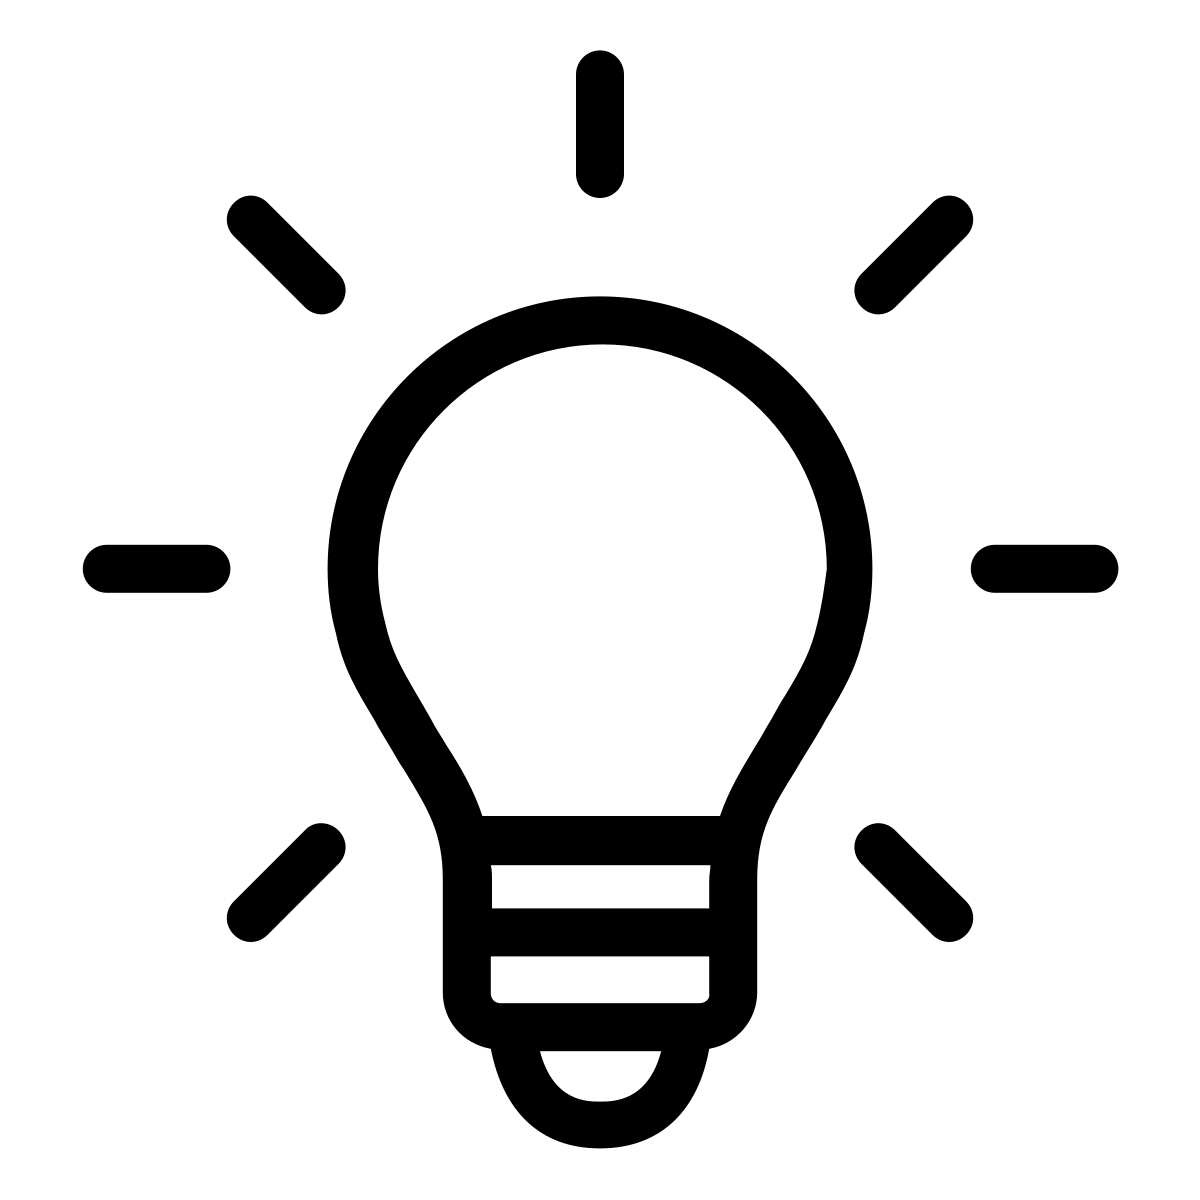
\includegraphics[width=0.36458in,height=\textheight]{images/bulb.png} Data Tip

\begin{quote}
\textbf{Why create a new variable when recoding?}\\
If you have a sharp eye, you'll notice that we created a new variable rather than changing the name of our original variable and recoding it. Data cleaning is an iterative process. You may make mistakes (you will probably make mistakes) or you may change your mind about how to recode a variable. In each case, having the original variable on hand is always helpful. To preserve your original variable, you create a new variable rather than writing over the old one.
\end{quote}

\hypertarget{vizualizing-variables-1}{%
\subsection*{Vizualizing variables}\label{vizualizing-variables-1}}
\addcontentsline{toc}{subsection}{Vizualizing variables}

\hypertarget{continuous-variables-1}{%
\subsubsection*{Continuous Variables}\label{continuous-variables-1}}
\addcontentsline{toc}{subsubsection}{Continuous Variables}

While frequency tables and descriptive statistics are helpful, visualizing continuous variables or discrete variables with a wide range of values can be helpful to get a look at the shape of our data. Histograms or box plots the go to.

There are two main ways to create graphs in R, base R plots and \texttt{ggplot2}. \texttt{ggplot2} has far more flexibility, so we will focus on that package primarily. However, when you are moving fast it can sometimes be helpful to throw up a quick histogram in base R.

\hypertarget{hist}{%
\paragraph*{\texorpdfstring{\texttt{hist()} Create a histogram in base R}{hist() Create a histogram in base R}}\label{hist}}
\addcontentsline{toc}{paragraph}{\texttt{hist()} Create a histogram in base R}

The code for creating a histogram using base R is simple, but you don't have as much flexibility to change aspects of the plot if you want to use it in presentations or papers.

\begin{Shaded}
\begin{Highlighting}[]
\FunctionTok{hist}\NormalTok{(mydata}\SpecialCharTok{$}\NormalTok{age)}
\end{Highlighting}
\end{Shaded}

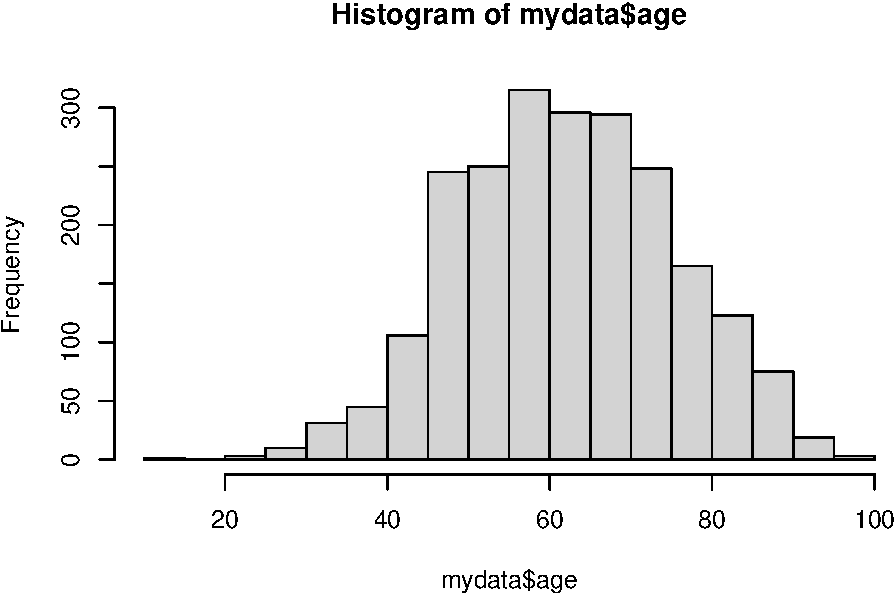
\includegraphics{_main_files/figure-latex/unnamed-chunk-35-1.pdf}

If you want to change the number of bins (i.e.~bars), you add a breaks argument to the function.

\begin{Shaded}
\begin{Highlighting}[]
\FunctionTok{hist}\NormalTok{(mydata}\SpecialCharTok{$}\NormalTok{age, }\AttributeTok{breaks =} \DecValTok{10}\NormalTok{)}
\end{Highlighting}
\end{Shaded}

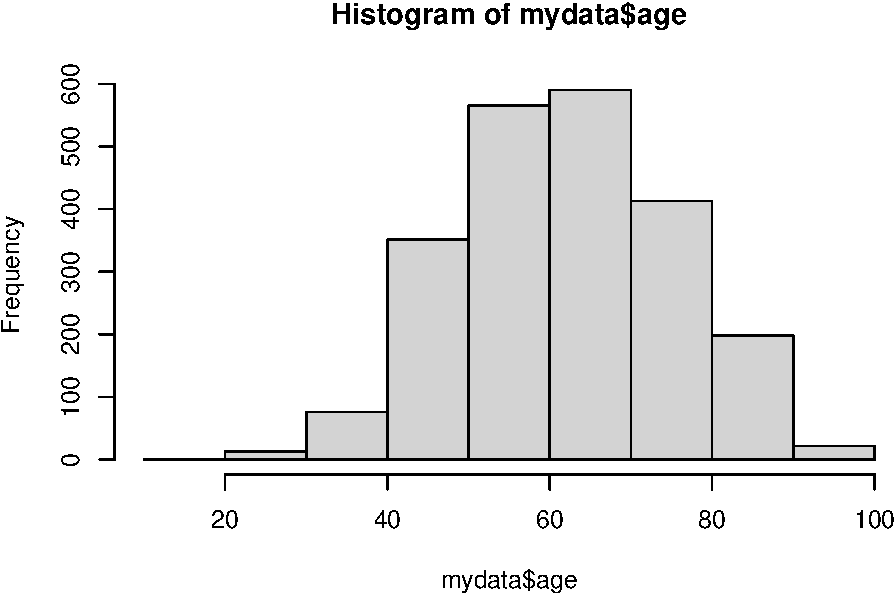
\includegraphics{_main_files/figure-latex/unnamed-chunk-36-1.pdf}

\hypertarget{histgg}{%
\paragraph*{\texorpdfstring{Histograms in \texttt{ggplot2}}{Histograms in ggplot2}}\label{histgg}}
\addcontentsline{toc}{paragraph}{Histograms in \texttt{ggplot2}}

As I've mentioned, \texttt{ggplot2} has a massive amount of flexibility and a unique grammar to building plots. It is the go-to package to produce quality plots and graphics, but is a lot to learn to use it with ease. If you are interested I recommend taking a \texttt{ggplot2} workshop or working through the \texttt{ggplot2} book listed in resources at the beginning of this lab. For now, let's build a simple histogram using the \texttt{ggplot()} function.

\begin{Shaded}
\begin{Highlighting}[]
\CommentTok{\# Creatign the plot}
\FunctionTok{ggplot}\NormalTok{(}\AttributeTok{data =}\NormalTok{ mydata, }\FunctionTok{aes}\NormalTok{(}\AttributeTok{x =}\NormalTok{ age)) }\SpecialCharTok{+} \CommentTok{\#specifying dataset and your variable}
  \FunctionTok{geom\_histogram}\NormalTok{(}\AttributeTok{color =} \StringTok{"white"}\NormalTok{) }\SpecialCharTok{+} \CommentTok{\#changing the outline of the bars to white}
  \FunctionTok{theme\_minimal}\NormalTok{() }\CommentTok{\# applying a built{-}in theme to the graph}
\end{Highlighting}
\end{Shaded}

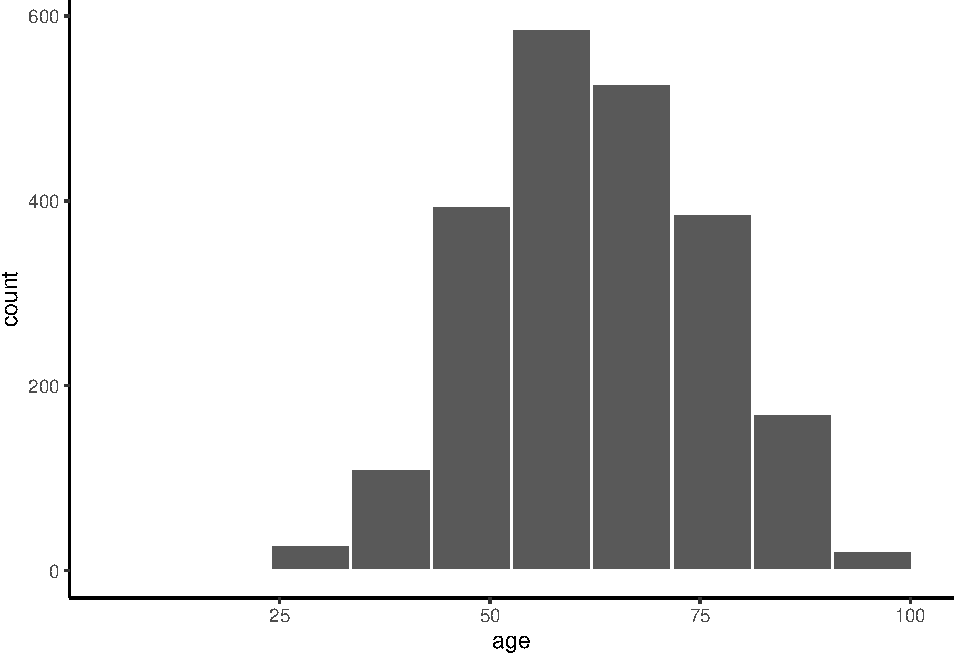
\includegraphics{_main_files/figure-latex/unnamed-chunk-37-1.pdf}

Let's try changing the number of bins.

\begin{Shaded}
\begin{Highlighting}[]
\FunctionTok{ggplot}\NormalTok{(}\AttributeTok{data =}\NormalTok{ mydata, }\FunctionTok{aes}\NormalTok{(}\AttributeTok{x =}\NormalTok{ age)) }\SpecialCharTok{+}
  \FunctionTok{geom\_histogram}\NormalTok{(}\AttributeTok{color =} \StringTok{"white"}\NormalTok{, }\AttributeTok{bins =} \DecValTok{10}\NormalTok{) }\SpecialCharTok{+}
  \FunctionTok{theme\_minimal}\NormalTok{()}
\end{Highlighting}
\end{Shaded}

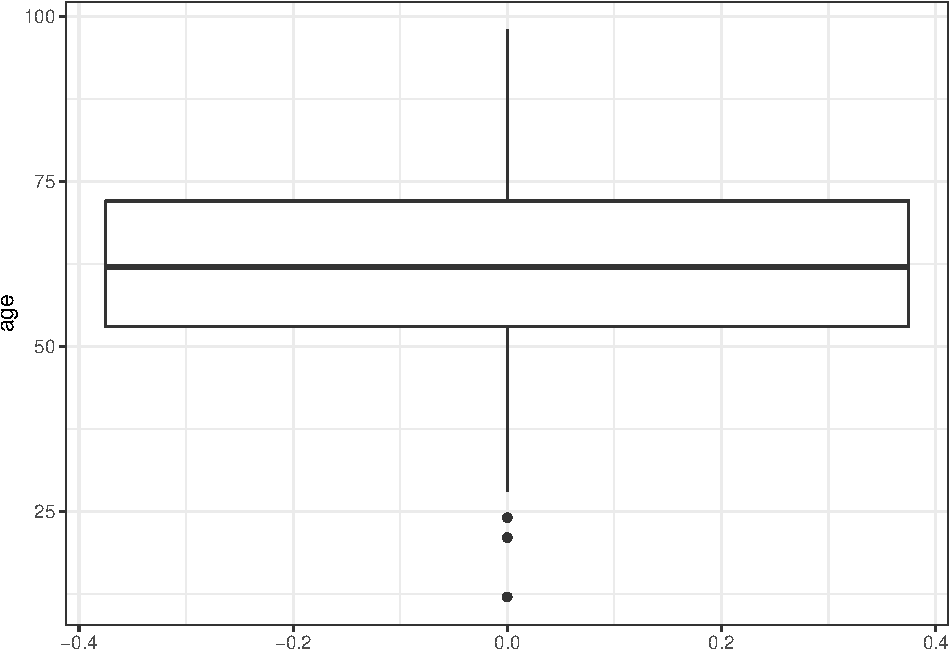
\includegraphics{_main_files/figure-latex/unnamed-chunk-38-1.pdf}

\hypertarget{boxplot}{%
\paragraph*{\texorpdfstring{Box plots with \texttt{ggplot()}}{Box plots with ggplot()}}\label{boxplot}}
\addcontentsline{toc}{paragraph}{Box plots with \texttt{ggplot()}}

Let's try making a boxplot of age.

\begin{Shaded}
\begin{Highlighting}[]
\FunctionTok{ggplot}\NormalTok{(}\AttributeTok{data =}\NormalTok{ mydata, }\FunctionTok{aes}\NormalTok{(}\AttributeTok{y =}\NormalTok{ age)) }\SpecialCharTok{+} \CommentTok{\# Calling the same data, but switched to y axis so the boxplot would be vertical}
  \FunctionTok{geom\_boxplot}\NormalTok{() }\SpecialCharTok{+} \CommentTok{\# calling the boxplot geom}
  \FunctionTok{theme\_bw}\NormalTok{() }\CommentTok{\# trying a different theme}
\end{Highlighting}
\end{Shaded}

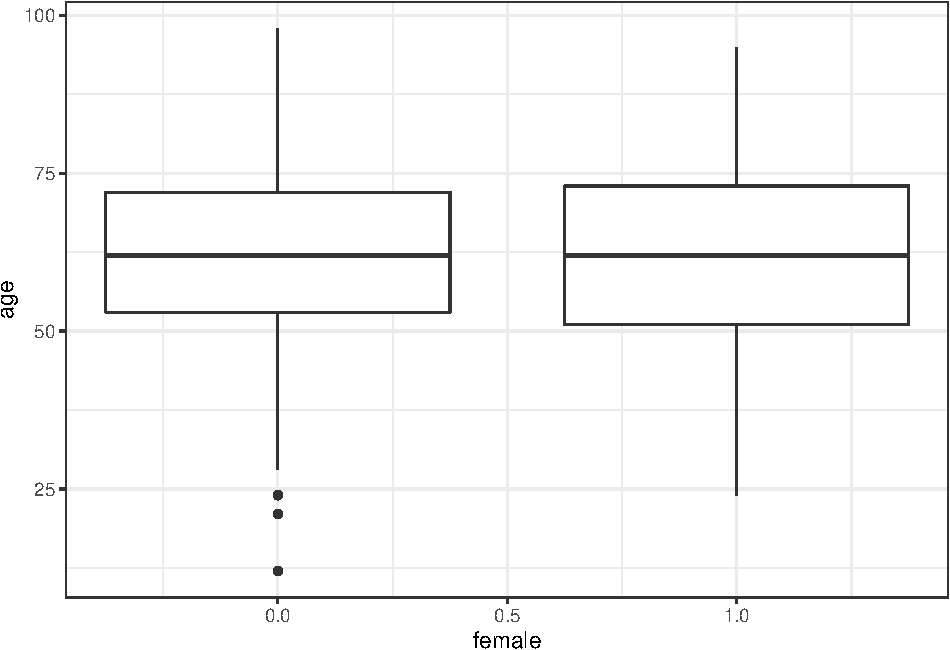
\includegraphics{_main_files/figure-latex/unnamed-chunk-39-1.pdf}

Let's try making a boxplot of age by gender.

\begin{Shaded}
\begin{Highlighting}[]
\FunctionTok{ggplot}\NormalTok{(}\AttributeTok{data =}\NormalTok{ mydata, }\FunctionTok{aes}\NormalTok{(}\AttributeTok{y =}\NormalTok{ age, }\AttributeTok{x =}\NormalTok{ female, }\AttributeTok{group =}\NormalTok{ female)) }\SpecialCharTok{+} 
  \CommentTok{\# adding x to label the x axis, and grouping by the same variable to create two box plots}
  \FunctionTok{geom\_boxplot}\NormalTok{() }\SpecialCharTok{+} \CommentTok{\# same geom}
  \FunctionTok{theme\_bw}\NormalTok{() }\CommentTok{\#same theme}
\end{Highlighting}
\end{Shaded}

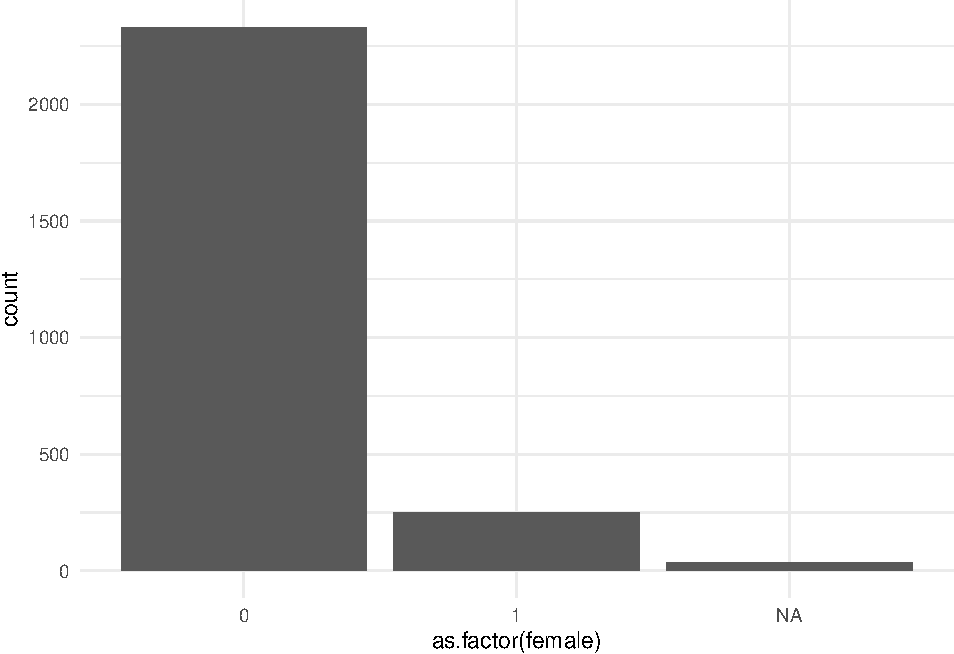
\includegraphics{_main_files/figure-latex/unnamed-chunk-40-1.pdf}

\hypertarget{categorical-variables-1}{%
\subsubsection{Categorical Variables}\label{categorical-variables-1}}

Again frequency tables are great, but sometimes a visualization of a categorical data can better communicate patterns.

\hypertarget{barplot}{%
\paragraph*{\texorpdfstring{Bar plots with \texttt{ggplot()}}{Bar plots with ggplot()}}\label{barplot}}
\addcontentsline{toc}{paragraph}{Bar plots with \texttt{ggplot()}}

Let's try making a bar plot of gender. Note I have to turn \texttt{female} into a factor. This doesn't permanently transform the variable. It just temporarily transforms the variable for this plot.

\begin{Shaded}
\begin{Highlighting}[]
\FunctionTok{ggplot}\NormalTok{(}\AttributeTok{data =}\NormalTok{ mydata, }\FunctionTok{aes}\NormalTok{(}\AttributeTok{x =} \FunctionTok{as.factor}\NormalTok{(female))) }\SpecialCharTok{+} 
  \FunctionTok{geom\_bar}\NormalTok{() }\SpecialCharTok{+} 
  \FunctionTok{theme\_classic}\NormalTok{()}
\end{Highlighting}
\end{Shaded}

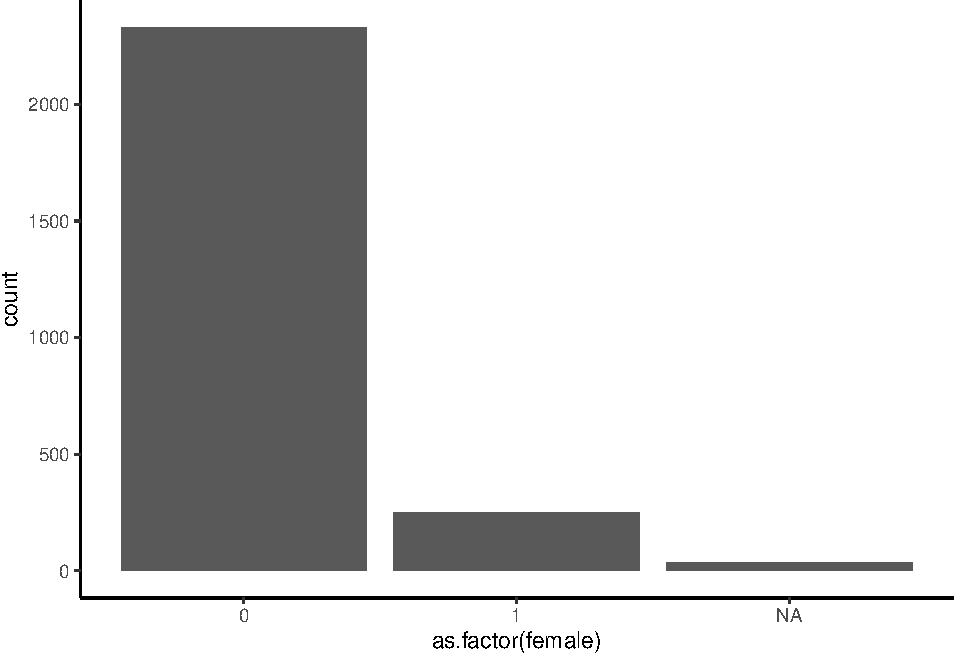
\includegraphics{_main_files/figure-latex/unnamed-chunk-41-1.pdf}

If I want to remove the NA column, I can also filter the data within the \texttt{ggplot} function. I'm also going to clean up the axis labels, add a title, and change the width of the bars.

\begin{Shaded}
\begin{Highlighting}[]
\FunctionTok{ggplot}\NormalTok{(}\AttributeTok{data =}\NormalTok{ mydata }\SpecialCharTok{\%\textgreater{}\%} \FunctionTok{drop\_na}\NormalTok{(female), }\FunctionTok{aes}\NormalTok{(}\AttributeTok{x =} \FunctionTok{as.factor}\NormalTok{(female))) }\SpecialCharTok{+} 
  \FunctionTok{geom\_bar}\NormalTok{(}\AttributeTok{width =}\NormalTok{ .}\DecValTok{5}\NormalTok{) }\SpecialCharTok{+} 
  \FunctionTok{labs}\NormalTok{(}
    \AttributeTok{x =} \StringTok{"Gender"}\NormalTok{, }
    \AttributeTok{y =} \StringTok{"Count"}\NormalTok{, }
    \AttributeTok{title =} \StringTok{"Bar plot of gender"}
\NormalTok{  ) }\SpecialCharTok{+} 
  \FunctionTok{theme\_classic}\NormalTok{()}
\end{Highlighting}
\end{Shaded}

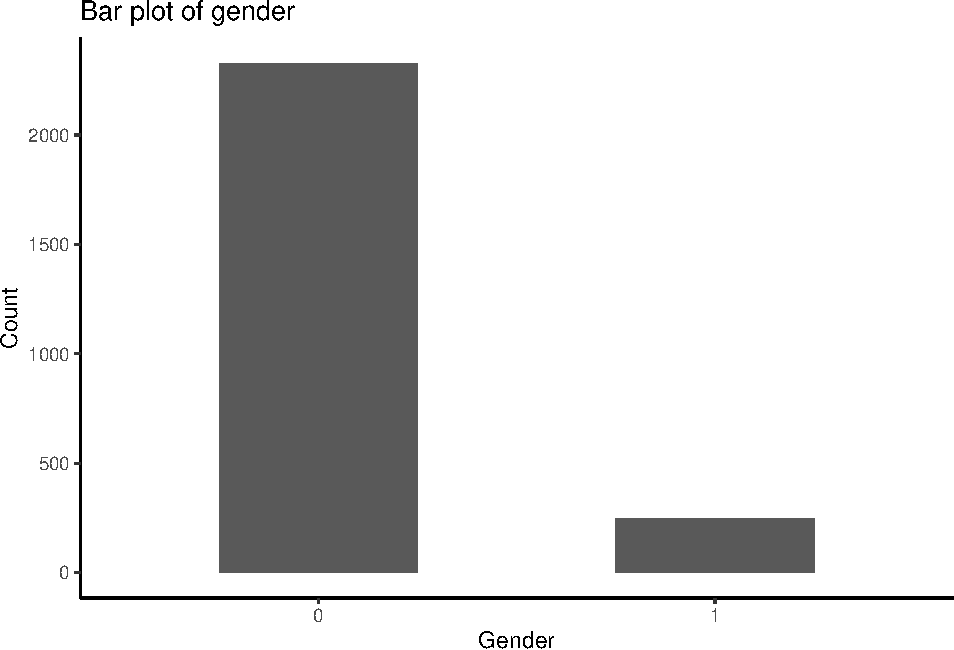
\includegraphics{_main_files/figure-latex/unnamed-chunk-42-1.pdf}

Another advantage of ggplot is that the code to save is much easier than base R plots. This code will save the last ggplot that you created. I encourage you to look up other examples of \texttt{ggsave} to learn different ways you can save plots as objects, specify height and width, and more.

\begin{Shaded}
\begin{Highlighting}[]
\FunctionTok{ggsave}\NormalTok{(}\StringTok{"figs\_output/barplot{-}example.png"}\NormalTok{)}
\end{Highlighting}
\end{Shaded}

\hypertarget{subsetting-and-saving-data-1}{%
\subsection*{Subsetting and saving data}\label{subsetting-and-saving-data-1}}
\addcontentsline{toc}{subsection}{Subsetting and saving data}

Sometimes you'll be working with a huge dataset, and it is easier and cleaner save portion of observations and/or variables in a new dataset. This is called a sub-sample.

\hypertarget{select}{%
\subsubsection*{\texorpdfstring{\texttt{select()} to subset your data to specific variables}{select() to subset your data to specific variables}}\label{select}}
\addcontentsline{toc}{subsubsection}{\texttt{select()} to subset your data to specific variables}

Let's say you only want to keep the following three variables: year and the two variables you just created: age and female. You can easily subset the data using the \texttt{select()} function in tidyverse. In the select function you simply list the variables you want to keep. You can also specify specific variables to drop by putting them in the list with a minus sign in front (example: \texttt{-year,\ -age,\ -female})

\begin{Shaded}
\begin{Highlighting}[]
\NormalTok{mysubset }\OtherTok{\textless{}{-}}\NormalTok{ mydata }\SpecialCharTok{\%\textgreater{}\%} \CommentTok{\# note I\textquotesingle{}m saving this as a new dataframe with a new name}
  \FunctionTok{select}\NormalTok{(year, age, female)}

\FunctionTok{skim\_without\_charts}\NormalTok{(mysubset) }\CommentTok{\# you should always check your data when you make a major change like adding or removing variables.}
\end{Highlighting}
\end{Shaded}

\begin{verbatim}
Error in kable_latex(x = structure(c("Name", "Number of rows", "Number of columns", : unused argument (table.attr = "style='width: auto;'\n        class='table table-condensed'")
\end{verbatim}

\hypertarget{filter}{%
\subsubsection*{\texorpdfstring{\texttt{filter()} to subset your data to specific observations}{filter() to subset your data to specific observations}}\label{filter}}
\addcontentsline{toc}{subsubsection}{\texttt{filter()} to subset your data to specific observations}

But what if you wanted to subset the data to only billionaires 30 or older? For this task, you can use the \texttt{filter()} function. Filter acts exactly like the name implies. Use a conditional statement to specify what observations you want to keep or remove from your dataset.

\begin{Shaded}
\begin{Highlighting}[]
\CommentTok{\# Filtering data to only billionaires over 30}
\NormalTok{mysubset2 }\OtherTok{\textless{}{-}}\NormalTok{ mydata }\SpecialCharTok{\%\textgreater{}\%}
  \FunctionTok{filter}\NormalTok{(age }\SpecialCharTok{\textgreater{}=} \DecValTok{30}\NormalTok{)}

\FunctionTok{range}\NormalTok{(mysubset2}\SpecialCharTok{$}\NormalTok{age) }\CommentTok{\# Another check to see our code worked how we wanted it!}
\end{Highlighting}
\end{Shaded}

\begin{verbatim}
[1] 30 98
\end{verbatim}

\hypertarget{save}{%
\subsubsection*{Saving your subset}\label{save}}
\addcontentsline{toc}{subsubsection}{Saving your subset}

Now that you have your subset, you'll want to save it. Saving in R's data, format is simple.

\begin{Shaded}
\begin{Highlighting}[]
\CommentTok{\# Saving as r data format (.rda or .rData {-} both are the same).}
\FunctionTok{save}\NormalTok{(mysubset, }\AttributeTok{file =} \StringTok{"data\_work/mysubset.rda"}\NormalTok{) }\CommentTok{\# note I\textquotesingle{}m saving this in my working data folder}
\end{Highlighting}
\end{Shaded}

There are extra steps to save it other formats. .CSV files, are one of the most common formats you'll receive and save data in outside of R.

\begin{Shaded}
\begin{Highlighting}[]
\FunctionTok{write\_csv}\NormalTok{(mysubset, }\AttributeTok{file =} \StringTok{"data\_work/mysubset.csv"}\NormalTok{)}
\end{Highlighting}
\end{Shaded}

\textbf{Remember}, every time you run these command it writes over your previous save. So be careful about version control and \textbf{ALWAYS} maintain the raw data file in a separate location.

\hypertarget{annotate}{%
\section{The Importance of Annotation and Clean Code}\label{annotate}}

A script is not just a functional document where you conduct your analysis. It is also an important record of your analysis. When you read back through your script files you should be able to understand what each step of code is doing and why. Well-written code scripts:

\begin{itemize}
\tightlist
\item
  Have a header with your name and a title or a short description of what the script contains (e.g., ``Cleaning data for regression analysis on billionaires'')
\item
  Document the analytic decisions made about cleaning and analysis
\item
  Can be run from start to finish without errors
\end{itemize}

You may think that you will remember what you were thinking when you wrote a script, but sometimes you'll have to step away from an analysis for weeks or months. When you come back to it, your notes will remind you exactly why you coded things the way you did. Your code scripts will also be read by other people. It may be collaborators, advisers, or colleagues who agree to quality check your code to look for errors. It is also more and more common for journals to ask scholars to post their coding files so that other people can replicate your analysis.

\hypertarget{how-to-make-notes-in-your-script-1}{%
\subsection*{How to make notes in your script}\label{how-to-make-notes-in-your-script-1}}
\addcontentsline{toc}{subsection}{How to make notes in your script}

The main way to make a note in an R script is to use the \texttt{\#}. You can put the \texttt{\#} at the beginning of the line or after a piece of code. Whatever you type after the \texttt{\#} will be colored green to indicate notation text that will not be run as code.

Let's return to our code to filter our data. In this code I note above the command what it is about to do. In the second command, I include a note one the same line to remind myself that I want to check to make sure the code I ran worked correctly.

\begin{Shaded}
\begin{Highlighting}[]
\CommentTok{\# Filtering data to only billionaires over 30}
\NormalTok{mysubset2 }\OtherTok{\textless{}{-}}\NormalTok{ mydata }\SpecialCharTok{\%\textgreater{}\%}
  \FunctionTok{filter}\NormalTok{(age }\SpecialCharTok{\textgreater{}=} \DecValTok{30}\NormalTok{)}

\FunctionTok{range}\NormalTok{(mysubset2}\SpecialCharTok{$}\NormalTok{age) }\CommentTok{\# Another check to see our code worked how we wanted it!}
\end{Highlighting}
\end{Shaded}

There's one trick that can be helpful when writing notes in R script. Say you have a note that will take multiple lines. For example, you may want to document the source of the data you are using. If you put a single quotation mark after the hashtag (\texttt{\#\textquotesingle{}}), R will automatically make the next line a comment when you press enter. It will work in regular .R scripts, but will not work in .Rmd files. Try it out!

\begin{Shaded}
\begin{Highlighting}[]
\CommentTok{\#\textquotesingle{} This is a comment. When I press enter...}
\CommentTok{\#\textquotesingle{} The next line will be a comment too.}
\CommentTok{\#\textquotesingle{}}
\end{Highlighting}
\end{Shaded}

Finally, sometimes you may want to ``comment out'' a couple lines of code, either temporarily while you are coding or because you want to keep a record of code you don't need to run again. R has a handy shortcut to let you turn a chunk of codes into comments and turn a chunk of comments into code. You do this by highlighting the chunk you want to comment in or out and typing \texttt{Cmnd\ +\ Shift\ +\ C}. For example, in the following code, I want to remove the line of code that adds a title to my ggplot. I may want to add it back in later, so rather than removing the line of code, I just commented it out. The grammar of \texttt{tidyverse} and \texttt{ggplot2}, with their pipes and plus signs, make it easy to comment out a specific type of code.

\begin{Shaded}
\begin{Highlighting}[]
\FunctionTok{ggplot}\NormalTok{(}\AttributeTok{data =}\NormalTok{ mydata, }\FunctionTok{aes}\NormalTok{(}\AttributeTok{y =}\NormalTok{ age, }\AttributeTok{x =}\NormalTok{ female, }\AttributeTok{group =}\NormalTok{ female)) }\SpecialCharTok{+} 
  \FunctionTok{geom\_boxplot}\NormalTok{() }\SpecialCharTok{+} 
  \CommentTok{\# labs(}
  \CommentTok{\#   title = "Boxplot of age by gender"}
  \CommentTok{\# ) + }
  \FunctionTok{theme\_bw}\NormalTok{() }
\end{Highlighting}
\end{Shaded}

\hypertarget{tips-for-neat-code-1}{%
\subsection*{Tips for Neat Code}\label{tips-for-neat-code-1}}
\addcontentsline{toc}{subsection}{Tips for Neat Code}

Notes are a huge part of making your code readable to yourself and others. However, writing neat code is also an enormous gift you can give to yourself, to the TA grading your scripts, and anyone else trying to make sense of your code. Here are my top tips for writing neat code in R:

\begin{itemize}
\tightlist
\item
  Split long functions and commands across multiple lines
\item
  Leave spaces around equals signs and other operators
\item
  Create headers and sections in your code
\item
  Create clear names for your variables, data frames, and objects
\end{itemize}

\hypertarget{split-long-functions-and-commands-across-multiple-lines-1}{%
\subsubsection*{Split long functions and commands across multiple lines}\label{split-long-functions-and-commands-across-multiple-lines-1}}
\addcontentsline{toc}{subsubsection}{Split long functions and commands across multiple lines}

Nothing, I repeat, nothing makes code harder to read than shoving it all into one long line. R doesn't care how many lines you split code across. It will run a function until it gets to the last closed parentheses. Splitting code across multiple lines makes it easier for you to see and edit your code. It makes it way more legible to others reading your code. Look at the difference between these two pairs of commands from earlier in this lab.

\begin{Shaded}
\begin{Highlighting}[]
\CommentTok{\# Creating a frequency table with percentages }
\NormalTok{mydata }\SpecialCharTok{\%\textgreater{}\%} \FunctionTok{group\_by}\NormalTok{(year) }\SpecialCharTok{\%\textgreater{}\%} \FunctionTok{count}\NormalTok{() }\SpecialCharTok{\%\textgreater{}\%} \FunctionTok{mutate}\NormalTok{(}\AttributeTok{percent =} \FunctionTok{round}\NormalTok{(n }\SpecialCharTok{/} \FunctionTok{nrow}\NormalTok{(mydata) }\SpecialCharTok{*} \DecValTok{100}\NormalTok{, }\DecValTok{2}\NormalTok{))}

\CommentTok{\# Creating a boxplot with a title }
\FunctionTok{ggplot}\NormalTok{(}\AttributeTok{data =}\NormalTok{ mydata, }\FunctionTok{aes}\NormalTok{(}\AttributeTok{y =}\NormalTok{ age, }\AttributeTok{x =}\NormalTok{ female, }\AttributeTok{group =}\NormalTok{ female)) }\SpecialCharTok{+} \FunctionTok{geom\_boxplot}\NormalTok{() }\SpecialCharTok{+} \FunctionTok{labs}\NormalTok{(}\AttributeTok{title =} \StringTok{"Boxplot of age by gender"}\NormalTok{) }\SpecialCharTok{+} \FunctionTok{theme\_bw}\NormalTok{() }
\end{Highlighting}
\end{Shaded}

These lines of code will run just fine, but they are difficult for your eye to parse when squished together. Let your code breathe! Notice how in the clean version of this code below, I even split the \texttt{labs()} function across three lines. This may not matter as much here, but if I add an x axis label, y axis label, subtitle, and caption, I would put each on its own line for ease of reading and editing.

\begin{Shaded}
\begin{Highlighting}[]
\NormalTok{mydata }\SpecialCharTok{\%\textgreater{}\%}
  \FunctionTok{group\_by}\NormalTok{(year) }\SpecialCharTok{\%\textgreater{}\%}
  \FunctionTok{count}\NormalTok{() }\SpecialCharTok{\%\textgreater{}\%}
  \FunctionTok{mutate}\NormalTok{(}\AttributeTok{percent =} \FunctionTok{round}\NormalTok{(n }\SpecialCharTok{/} \FunctionTok{nrow}\NormalTok{(mydata) }\SpecialCharTok{*} \DecValTok{100}\NormalTok{, }\DecValTok{2}\NormalTok{))}

\FunctionTok{ggplot}\NormalTok{(}\AttributeTok{data =}\NormalTok{ mydata, }\FunctionTok{aes}\NormalTok{(}\AttributeTok{y =}\NormalTok{ age, }\AttributeTok{x =}\NormalTok{ female, }\AttributeTok{group =}\NormalTok{ female)) }\SpecialCharTok{+} 
  \FunctionTok{geom\_boxplot}\NormalTok{() }\SpecialCharTok{+} 
  \CommentTok{\# labs(}
  \CommentTok{\#   title = "Boxplot of age by gender"}
  \CommentTok{\# ) + }
  \FunctionTok{theme\_bw}\NormalTok{() }
\end{Highlighting}
\end{Shaded}

As a rule, don't let any line get past about 80 characters. RStudio includes a
vertical line at about this point. I recommend that you don't write past it in
your code scripts. It will help you and the reader avoid the annoying horizontal scroll bar.

\hypertarget{leave-spaces-around-operators-1}{%
\subsubsection*{Leave spaces around operators}\label{leave-spaces-around-operators-1}}
\addcontentsline{toc}{subsubsection}{Leave spaces around operators}

This is another tip to let your code breathe! When coding it is best practice to
put a space after any comma or logical operator. Take the line of code below:

\begin{Shaded}
\begin{Highlighting}[]
\FunctionTok{mutate}\NormalTok{(}\AttributeTok{percent=}\FunctionTok{round}\NormalTok{(n}\SpecialCharTok{/}\FunctionTok{nrow}\NormalTok{(mydata)}\SpecialCharTok{*}\DecValTok{100}\NormalTok{,}\DecValTok{2}\NormalTok{))}
\end{Highlighting}
\end{Shaded}

It works, but it's cluttered and makes it difficult to read. Take a look at this
line in a cleaner format:

\begin{Shaded}
\begin{Highlighting}[]
\FunctionTok{mutate}\NormalTok{(}\AttributeTok{percent =} \FunctionTok{round}\NormalTok{(n }\SpecialCharTok{/} \FunctionTok{nrow}\NormalTok{(mydata) }\SpecialCharTok{*} \DecValTok{100}\NormalTok{, }\DecValTok{2}\NormalTok{))}
\end{Highlighting}
\end{Shaded}

Notice how I've added a space on both sides of the \texttt{=}, the \texttt{/}, and the \texttt{*}. This makes it easier to understand and edit your code.

\hypertarget{create-headers-and-sections-in-your-code-1}{%
\subsubsection*{Create headers and sections in your code}\label{create-headers-and-sections-in-your-code-1}}
\addcontentsline{toc}{subsubsection}{Create headers and sections in your code}

You wouldn't write a paper without any titles or sections, so don't write your code without titles or sections! Take a look back at the R script for this lab. Notice how I put a section header for setting up your environment, exploring your data, cleaning your data, and so on. Hopefully this made it easier for you to work through the script.

You can create headers with comments, but you can also use a shortcut built into R. If you go to \textbf{Code -\textgreater{} Insert Section} or \texttt{Ctrl+Shift+R} (\texttt{Cmd+Shift+R} on the Mac). This will insert a header and create a code section. Any comment line which includes at least four trailing dashes (-), equal signs (=), or pound signs (\#) automatically creates a code section.

\begin{Shaded}
\begin{Highlighting}[]
 \CommentTok{\# Section One {-}{-}{-}{-}{-}{-}{-}{-}{-}{-}{-}{-}{-}{-}{-}{-}{-}{-}{-}{-}{-}{-}{-}{-}{-}{-}{-}{-}{-}{-}{-}{-}{-}}
 
 \CommentTok{\# Section Two =================================}
 
 \DocumentationTok{\#\#\# Section Three \#\#\#\#\#\#\#\#\#\#\#\#\#\#\#\#\#\#\#\#\#\#\#\#\#\#\#\#\# }
\end{Highlighting}
\end{Shaded}

You can collapse and expand code sections or use a drop down menu to jump to a code section. Trust me when I say cleaning scripts can get long, and these section headers can be a huge time-saver.

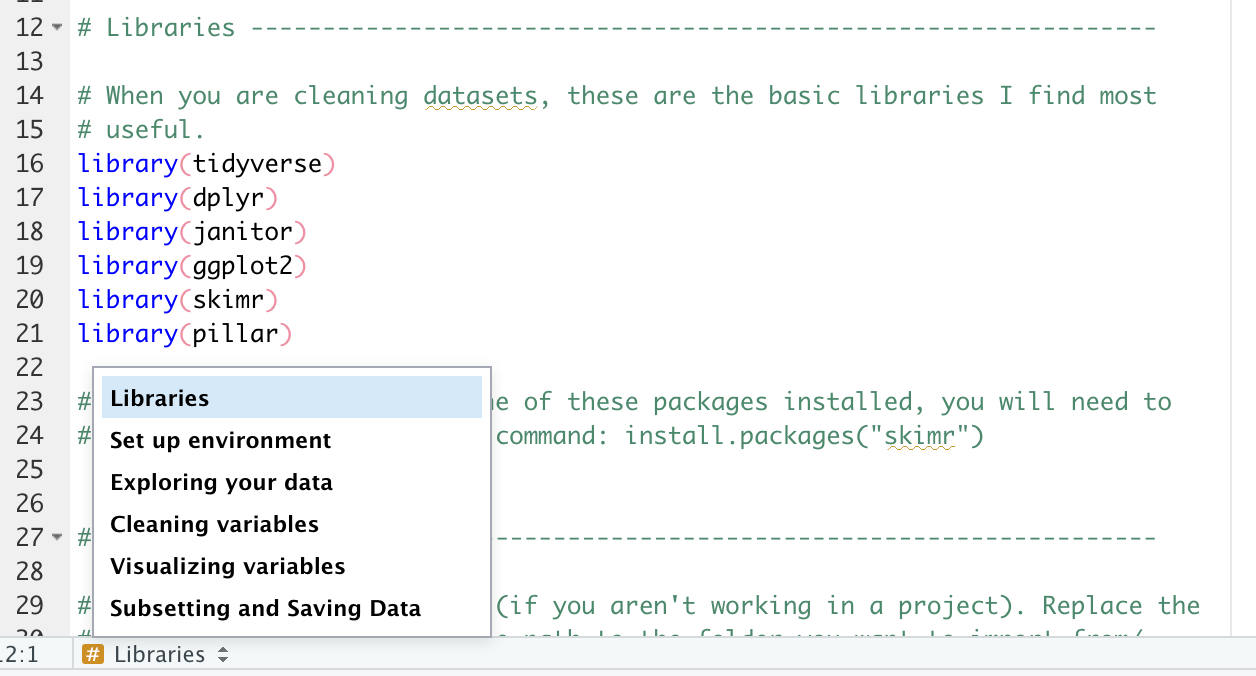
\includegraphics[width=0.75\linewidth]{images/jumpmenu}

\hypertarget{create-clear-names-for-your-variables-data-frames-and-objects}{%
\subsubsection*{Create clear names for your variables, data frames, and objects}\label{create-clear-names-for-your-variables-data-frames-and-objects}}
\addcontentsline{toc}{subsubsection}{Create clear names for your variables, data frames, and objects}

Everyone has their own preferred naming system for variables, data frames, and other R objects. The golden rule for naming is consistency. For example, if I recode variables I will often add \texttt{\_rc} to the end for recode (e.g., \texttt{age} and \texttt{age\_rc}). Other tips:\\
* Make your names explicit, but brief (e.g., \texttt{table\_1}, \texttt{table\_2})
* Don't include spaces in your file names, it makes file paths difficult

\hypertarget{activity-1}{%
\section{Activity}\label{activity-1}}

For this class, we expect you to write legible, clean code. To kick start this process, I want you to begin develop your own coding style. By class on Monday, email me (\texttt{rosewerth@u.northwestern.edu}) a script file for a hypothetical data cleaning script. The script should include:

\begin{enumerate}
\def\labelenumi{\arabic{enumi})}
\tightlist
\item
  A script header with your name, the date you created the script, and a short description of what the script contains
\item
  Two section headers
\item
  A note telling me what you find easy about coding in R and what you find difficult about coding in R.
\end{enumerate}

This should be your template for writing clean scripts for the rest of the quarter. Your template can evolve, but I expect all your scripts moving forward to contain title and section headers and clear annotation for each step in your code.

  \bibliography{book.bib,packages.bib}

\end{document}
